\chapter{\label{ch:7-qbo} The tropical route of QBO teleconnections in UKESM1 and HadGEM3 }

In this chapter, the influence of the QBO on the tropical mean circulation and teleconnections is examined in the pre-industrial control experiments of CMIP6 of the MOHC models. The relationship between the QBO and the tropical circulation, monsoons and the ITCZ is diagnosed and results are discussed in the context of existing observational evidence of QBO tropical teleconnections. 

%Secondly,  numerical experiments with the MOHC models were designed and performed to test the hypothesis thata relaxation of the zonal wind the equatorial stratosphere towards a reanalysis dataset are described and compared with free-running simulations.

\section{Introduction}

Long-distance effects or teleconnections associated with the stratospheric quasi-biennial oscillation (QBO) have been well documented in the subtropics and extratropics, for example for the stratospheric polar vortex \citep{holton1980,anstey2014,lu2020}, the subtropical jets \citep{garfinkel2011,hansen2016tropospheric} and the North Atlantic Oscillation \citep{hansen2016tropospheric,gray2018,andrews2019observed}.  
 Observational and modelling evidence suggests that there is also a tropical route of influence of the QBO to surface climate, for example, over tropical convective phenomena such as monsoons \citep{giorgetta1999,liess2012}, the ITCZ \citep{gray2018}, tropical cyclones \citep{gray1984,chan1995} and most recently, the Madden-Julian Oscillation (MJO) \citep{lee2018,wang2019,martin2020jgr}, see section \ref{sq:trop_qbo}. 
 
%Several observational and modelling studies have found evidence of QBO-related influence over convective activity in monsoon regions, such as in the South American, East Asian, Australian and Indian monsoons \citep{giorgetta1999,collimore2003,liess2012,gray2018} as well as over. 
In observations, surface impacts of the QBO over monsoon regions have been diagnosed in satellite-derived fields such as cloud height, occurrence and out-going longwave radiation \citep{collimore2003,liess2012}, as well as in surface precipitation diagnosed from gridded datasets or from reanalysis \citep{gray2018}.
However,  the observational evidence shows zonally asymmetric impacts, indicative that the impact of the QBO depends on longitude, which has been explained \citep[e.g. by][]{collimore2003,liess2012} through a QBO modulation of the Walker circulation.
In models,  \cite{giorgetta1999} find that boreal summer monsoon regions exhibit a significant response in cloudiness to QBO winds within the GCM ECHAM4. 
\cite{nie2015} find in a modelling framework that the influence of the QBO may depend on the strength of convection and SST forcing, suggesting a non-linear effect of the QBO over a convective profile.


 Although the polar and subtropical routes of influence of the QBO to the surface are relatively well established, the impact of the QBO over tropical convective phenomena remains less well understood for various reasons. The short observational record limits the confidence in any analysis that seeks to investigate differences between the two QBO phases in a 30-40-yr long dataset. Tropical circulation variability on QBO time-scales is largely dominated by ENSO and there is also evidence that ENSO and convection in the tropical Pacific influence the QBO, which makes it difficult to separate the cause and effects of ENSO and the QBO \citep{schirber2015,christiansen2016,gray2018}. In addition,  only a relatively small number of studies have analysed tropical QBO teleconnections in CMIP5/CMIP6 models \citep{serva2021}, as most CMIP analyses focus on the polar and subtropical routes of QBO influence \citep{richter2020,anstey2021}. 
 
 %Finally, , so there is a two-way relationship that would make difficult a separation of cause and effect \citep{schirber2015,christiansen2016}. 
 
 
Furthermore, the specific physical mechanisms through which the QBO could influence tropical convection at the grid-scale or the large-scale tropical circulation are also not well understood. 
While early studies \citep{gray1984,collimore2003} suggest that changes to the vertical wind shear or static stability in the upper-troposphere lower-stratosphere (UTLS) region are the cause of these teleconnections, there is a lack of evidence in the literature to support any mechanism over another. 
As such, studies have struggled to pin-point direct impacts and mechanisms by which the QBO may modulate any aspect of tropical climate. 

This chapter investigates QBO tropical teleconnections in the pre-industrial control simulations of the MOHC from CMIP6: GC3 N96-pi, GC3 N216-pi, UKESM-pi. Because these experiments are very long and external forcing is kept constant, and the UM reasonably simulates the QBO \citep{richter2020}, the impacts of internally-generated variability can be more easily examined. 
%   are ideal to investigate variability associated with the QBO because these experiments are very long integrations where external forcing is kept constant within the simulation and the 
%The remainder of this chapter is presented as follows. 
%First, the data and methods used are described, after which the results analysing the QBO impacts over the seasonal precipitation and surface temperatures  is given. 
%Then, a more detail investigation on the effects on the East Pacific and Atlantic ITCZs is presented and finally, the impacts over ENSO, the Indian Ocean and the Walker circulation are given. 
%A discussion is given at the end of the chapter.
% These simulations are examined first via composite analysis to investigate whether tropical convective phenomena such as the ITCZ and monsoon rainfall show any significant response to the state of the QBO. 





\section{Methods and data}

The observational datasets and reanalysis (ERA5) used in this chapter are described in section \ref{sq:obsdata} and consist of the HadSST3 dataset for SST, GPCP for precipitation and ERA5 for the rest of the diagnostics that include the zonal and meridional winds, air temperature, etc.

\subsection{CMIP6 data}

The three pre-industrial control experiments of the MOHC submitted to CMIP6 are used in this chapter: GC3 N96-pi, GC3 N216-pi and UKESM-pi. UKESM-pi and GC3 N96-pi are run with the same resolution (N96) of 1.875$^\circ$x1.25$^\circ$ and GC3 N216-pi is considered a medium-resolution simulation (N216) with atmospheric resolution of 0.83$^\circ$x 0.56$^\circ$. The period of 1850-2350 (500 years) is used for GC3 N96-pi and GC3 N216-pi and 2050-2650 (600 years) for the UKESM-pi. 
The three simulations chosen use the same model setup, with constant year 1850 forcing, but differ in their horizontal resolution or the treatment of aerosol-chemistry processes and land-surface interactions (see section \ref{sq:modeldata}). 

\subsection{Indices}

The indices for ENSO and the QBO are diagnosed exactly as in section \ref{sq:meth_ch4}, i.e., the 70-hPa zonal mean zonal wind index is used for the QBO with a threshold of 2 m s$^{-1}$ for each phase and the EN3.4 index is used with a threshold of $\pm$0.65 to define positive or negative events.

\subsection{Analysis techniques}

Composite analysis is the preferred technique used throughout this chapter. For each QBO or ENSO phase, composite samples are drawn for specific seasons using the indices and definitions mentioned above. 
Statistical significance is estimated in various ways, in some cases through standard Student or Welch t-test's where specified, and in some other cases a randomised resampling or bootstrapping method is also implemented in several sections of the chapter. 
The bootstrapping method is performed in all cases by drawing random samples from the entire simulation and repeating the process 10,000 times to evaluate the likelihood of obtaining a relationship by chance. 

Linear regression analysis has proven useful to understand the effect of one or more aspects of the climate over a region or a time-series, and was used to investigate the surface impacts of the QBO in observations by \cite{gray2018}. 
A simple linear regression model can be written as:

\begin{equation}
Y(t)=X_0+X_i(t)\beta_i + \epsilon,
\end{equation}
\noindent where $Y$ is the measured or dependent variable, $X_0$ is a constant coefficient, $\beta_i$ is the regression coefficient between $X_i$ and $Y$ and $\epsilon$ represents random error or a residual.  In all cases, the models solved using an ordinary least-squares (OLS) method.
A multivariate regression model can be used to study the joint effect of two or more predictors over a variable ($Y$) such that the model can be written as:
\begin{equation}
Y(t)=X_0+\sum_j^NX_j(t)\beta_j+\epsilon
\end{equation}
\noindent where $X_j(t)$ is any predictor with an associated regression coefficient $\beta_j$. 
As in previous studies \citep{gray2018,misios2019slowdown}, the regression coefficient can be rescaled to evaluate the total effect that a predictor ($X_j$) can have on the variance of the measured variable ($Y$) using the standard deviation ($\sigma_j$) and the maximum ($X_{j,max}$) and minimum ($X_{j_min}$) values of $X_j$ so that the rescaled coefficient $\beta_j^\prime$ can be written as:

\begin{equation}
\beta_j^\prime=\beta_j\frac{X_{j,max}-X_{j,min}}{\sigma_j}.
\end{equation}

\section{Teleconnections in the pre-industrial control experiments}\label{sq:cmip6_qbo}

\begin{figure}[b!]
\centering
 %\noindent
 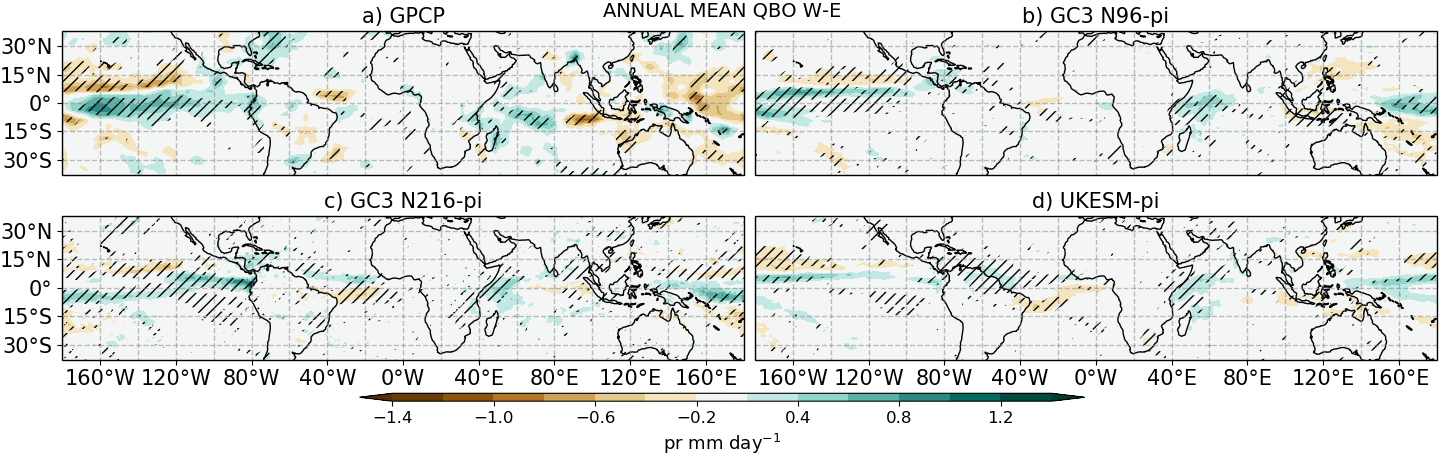
\includegraphics[width=\linewidth]{figures/piprclimqbowqboe.png}
\caption[Annual mean precipitation composite difference QBO W-E ]{ Annual mean precipitation difference between QBO W-E phases in (a) GPCP, (b) GC3 N96-pi, (c) GC3 N216-pi and (d) UKESM-pi. Hatching denotes statistical significance to the 95\% confidence level using bootstrapping with replacement for each composite sample. }
\label{fig:qboclim}
\end{figure}

%Surface impacts of the QBO in the tropics have scarcely been investigated in CMIP models, as most studies focus on the general representation of the QBO \citep[e.g][]{schenzinger2017,bushell2020}, or the extratropical teleconnections \citep[e.g.][]{anstey2021,dimdore2021}. 
%However, studies that have investigated teleconnections between the QBO and tropical convective phenomena in GCMs \citep[e.g.][]{lee2018,martin2021,serva2021} have found that model biases in representing the variability of temperature and winds in the tropopause layer may hinder a possible interaction between the QBO and tropical convection. 

This section examines more closely how the MOHC piControl experiments simulate the effect of the QBO over seasonal-mean precipitation, monsoons and the ITCZ. 



\subsection{Seasonal variability}

\begin{figure}[t!]
\centering
 %\noindent
 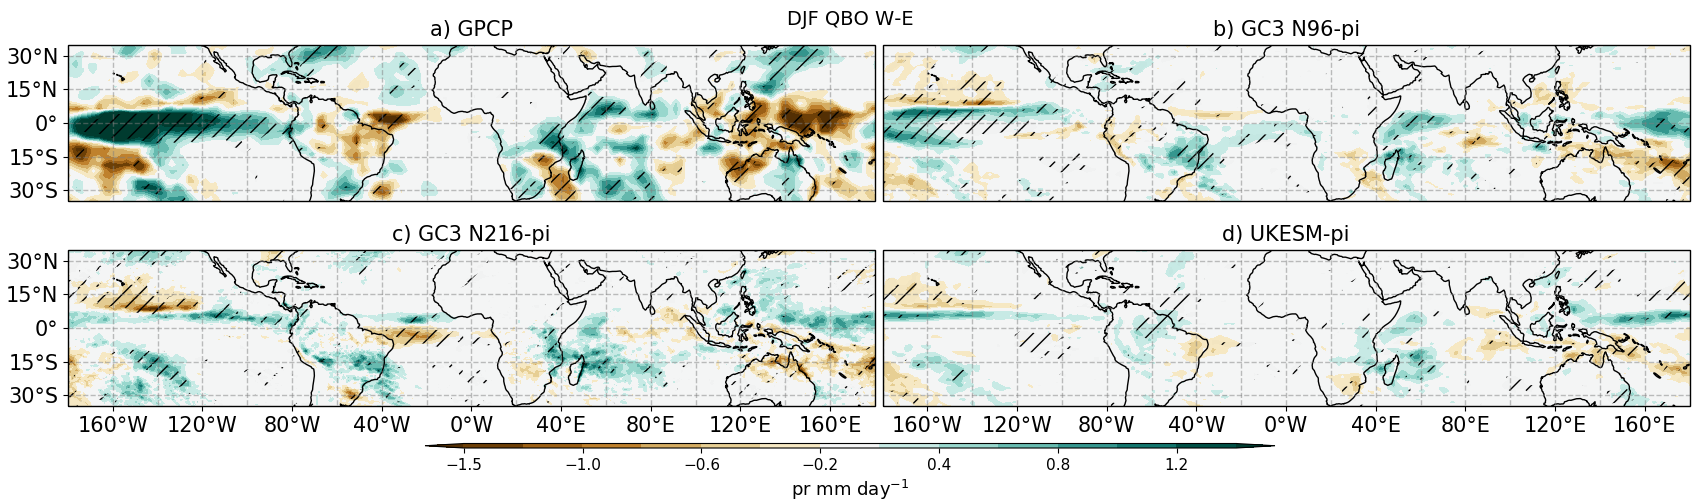
\includegraphics[width=\linewidth]{figures/piprdjfqbowqboe.png}
\caption[DJF mean precipitation composite difference QBO W-E ]{ As in Figure \ref{fig:qboclim} but for DJF. }
\label{fig:qbodjf}
\end{figure}

The composite difference in annual mean precipitation between QBO W and E phases (Figure \ref{fig:qboclim}) shows that in observations (GPCP) the tropical Pacific, equatorial Atlantic and the Indian Oceans are the regions of possibly largest influence of the QBO, which agrees with previous studies \citep{liess2012,gray2018}. The three GCM simulations agree well with the pattern in GPCP, as all three simulations show a positive difference (QBO W-E) in the Central Pacific and the Indian Ocean, albeit the differences are smaller in the simulations. However, the patterns and magnitudes of the impacts become larger when analysed over specific seasons. %, and in fact, the pattern exhibits strong seasonal variability. 

\begin{figure}[t!]
\centering
 %\noindent
 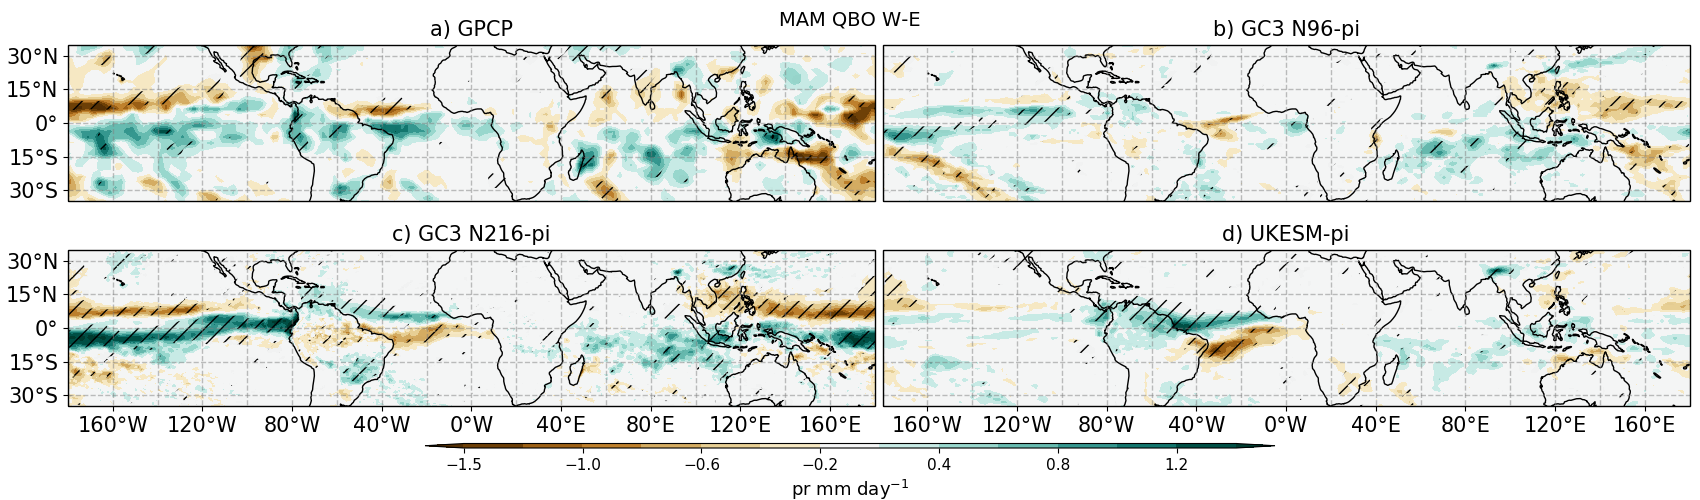
\includegraphics[width=\linewidth]{figures/piprmamqbowqboe.png}
\caption[MAM mean precipitation composite difference QBO W-E ]{ As in Figure \ref{fig:qboclim} but for MAM. }
\label{fig:qbomam}
\end{figure}

For example, during DJF (Figure \ref{fig:qbodjf}), the pattern over the Central Pacific is stronger in GPCP and the simulations relative to the annual mean difference. The positive difference in the western Indian Ocean and the South Pacific Convergence Zone is also observed in this season and is significant in all the datasets. Results in GC3 N216-pi suggest a weakening of the Atlantic ITCZ as in GPCP, whereas UKESM-pi and GC3 N96-pi show little and not significant responses in that region.
The response in the East Pacific during DJF matches the results of \cite{serva2021}, and suggests a southward shift of the ITCZ.
%had been previously 


Similarly, during MAM (Figure \ref{fig:qbomam}), the strongest response arises in the East Pacific and Atlantic ITCZ regions. In GC3 N216-pi the East Pacific ITCZ is shifted southwards whereas in the Atlantic the ITCZ is displaced northward. UKESM-pi agrees with the northward shift of the Atlantic ITCZ and suggests a wetter northern South America during QBO W than E. In GC3 N96-pi, the differences are smaller and the most noteworthy pattern is found in the Western Pacific. 
%Although the impact of the QBO over the ITCZ position has been previously described \citep{gray2018,serva2021}, less is known about the specific mechanisms leading to the change in position and strength of the ITCZ. 


\begin{figure}[t!]
\centering
 %\noindent
 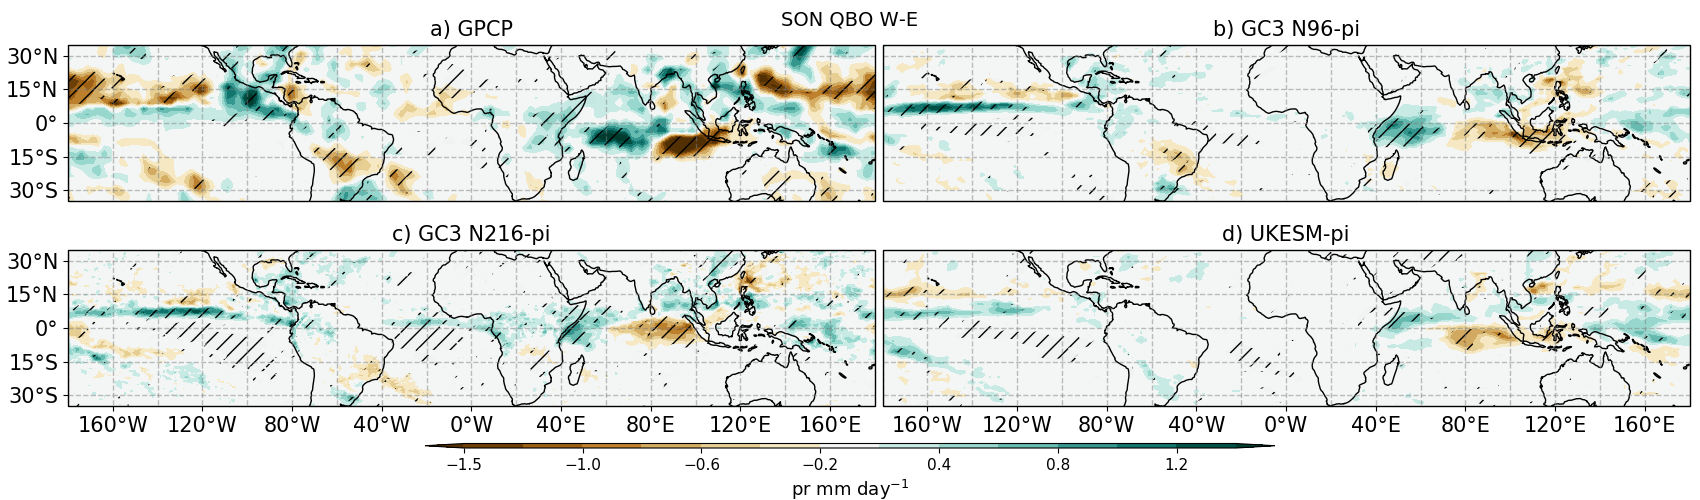
\includegraphics[width=\linewidth]{figures/piprsonqbowqboe.png}
\caption[SON mean precipitation composite difference QBO W-E ]{ As in Figure \ref{fig:qboclim} but for SON. }
\label{fig:qboson}
\end{figure}


In boreal fall (Figure \ref{fig:qboson}), all datasets show relatively large and significant differences in the Indian Ocean, characterized by a dipole of wet anomalies to the west and dry anomalies to the east. These dipole anomalies may be an indication that the QBO influences the Indian Ocean Dipole (IOD), characterized by a zonal gradient of SSTs in the Indian Ocean. In addition, results for GC3 N96-pi and GC3 N216-pi suggest a similar response in the Central and Eastern Pacific as in the other seasons, characterized by a wet anomaly at about 10$^\circ$N.

Finally, the JJA seasonal mean pattern (Figure \ref{fig:qbojja}) shows a weak response in GPCP whereas the simulations show a number of significant differences. Specifically, the three experiments suggest a wet anomaly in the Caribbean Sea and the Indian Ocean; the former, likely related to the northward shift of the Atlantic ITCZ observed in the same season particularly in UKESM-pi. West of the Caribbean Sea, in the easternmost Pacific Ocean a seemingly southward shift of the ITCZ is observed with a negative precipitation response on the western coast of Mexico.
A wetter Indian Ocean is observed in all the simulations and in UKESM-pi the wet anomaly extends over land into the Indian monsoon region.

\begin{figure}[t!]
\centering
 %\noindent
 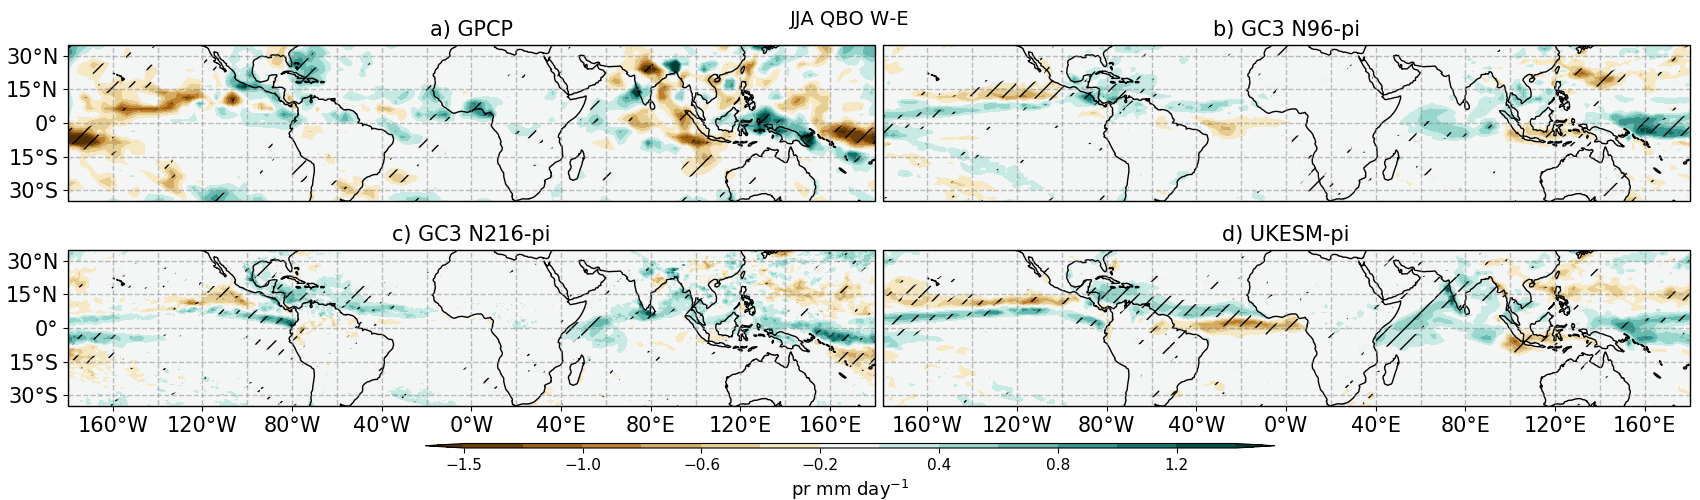
\includegraphics[width=\linewidth]{figures/piprjjaqbowqboe.png}
\caption[JJA mean precipitation composite difference QBO W-E ]{ As in Figure \ref{fig:qboclim} but for JJA. }
\label{fig:qbojja}
\end{figure}


 Note that in the annual and seasonal mean patterns there are little or no differences over land, except in JJA (Fig. \ref{fig:qbojja}) as a positive and significant response over land is observed in southern Mexico and Central America in all three simulations. Another positive and significant response is observed over the Indian monsoon region in JJA, although this signal is only present in UKESM-pi (Fig. \ref{fig:qbojja}d). 

\begin{figure}[t!]
\centering
 %\noindent
 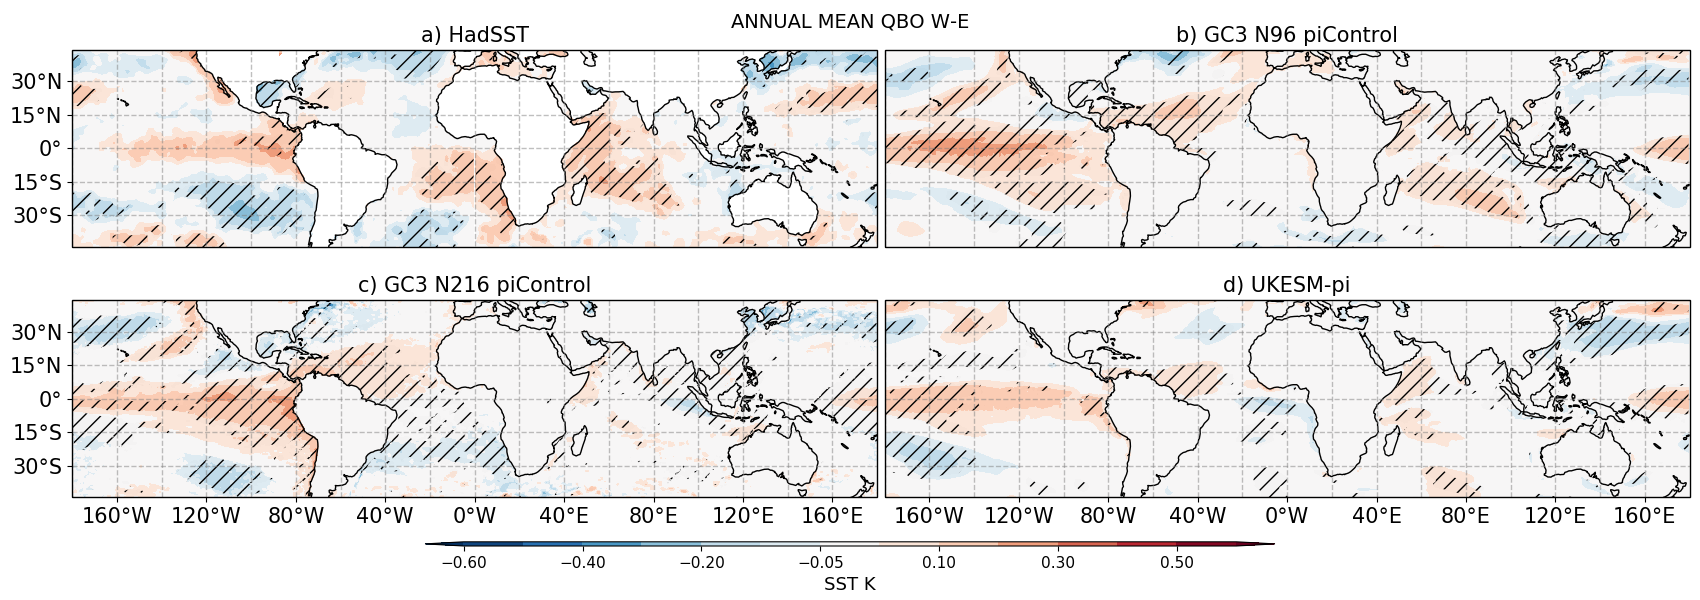
\includegraphics[width=\linewidth]{figures/pisstclimqbowqboe.png}
\caption[Annual mean SST difference QBO W-E under different QBO phases.]{ As in Figure \ref{fig:qboclim} but for SSTs.}
\label{fig:sstclim}
\end{figure}

The observed precipitation responses in the Central Pacific resemble an El Niño pattern especially during DJF (Fig. \ref{fig:qbodjf}) and in some simulations and seasons the El Niño pattern is also apparent. In observations, this pattern is likely a result of the increased frequency of El Niño events for QBOW than in QBOE \citep{liess2012}. 
For this reason, similar differences are obtained for SSTs (Figure \ref{fig:sstclim}) which show that  QBO W minus E SST differences appear as an El Niño pattern characterized by increased SSTs over the Central and Eastern Pacific, extending to the equatorial Atlantic. 
Although these differences are much weaker than the signal for a typical El Niño event, these differences are significant in all the simulations.% as well as in the HadSST dataset. 

\begin{figure}[t!]
\centering
 %\noindent
 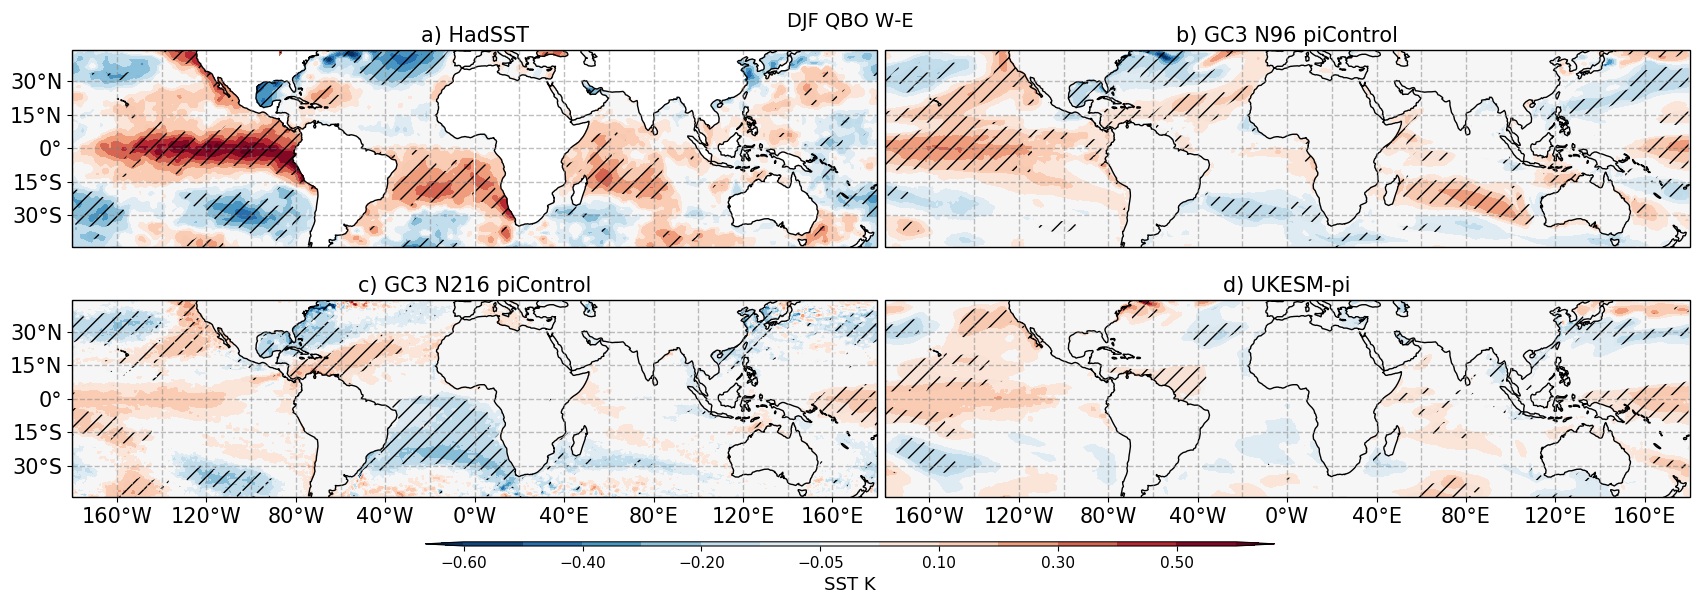
\includegraphics[width=\linewidth]{figures/pisstdjfqbowqboe.png}
\caption[DJF mean SST difference QBO W-E under different QBO phases.]{ As in Figure \ref{fig:sstclim} but for DJF.}
\label{fig:djfclim}
\end{figure}

The specific SST pattern for DJF confirms that the SST pattern seen in the annual mean difference is stronger during the boreal winter season, particularly for GC3 N96-pi and for the HadSST dataset. 
The observed SST anomaly pattern ressembles an East Pacific (or 'standard') El Niño, whereas the modelled anomalies look more like central Pacific El Niño. These SST differences probably explain the differences between the observed and modelled rainfall anomalies (as well as the observed SST pattern being stronger). The significant responses in GC3 N96-pi over the North Atlantic and in the Indian Ocean also agree very well with HadSST. 
In the case of GC3 N216-pi the strongest SST anomalies over the Central Pacific appear during MAM (not shown) whereas for UKESM-pi the pattern appears during La Niña events with litte-to-no response during other phases of ENSO (not shown).  

In summary, this section presented the seasonal mean response in precipitation to the phases of the QBO. The main responses in the models were the ITCZ shifts over the Pacific and Atlantic Oceans, but robust signals also suggest wetter conditions in the Indian Ocean and the Caribbean Sea during QBOW compared to QBOE. These results suggest a strong variation of the response with the seasons and with ENSO phase and little overall effect over land regions.
%For this reason, the following two sections more closely examine the effect of the QBO over the ITCZs in the East Pacific and Atlantic ITCZs, the Indian Ocean Dipole (IOD) and land-averaged precipitation over monsoon regions. 

\subsection{Impacts over the ITCZ and the monsoons}

\begin{figure}[t!]
\centering
 %\noindent
 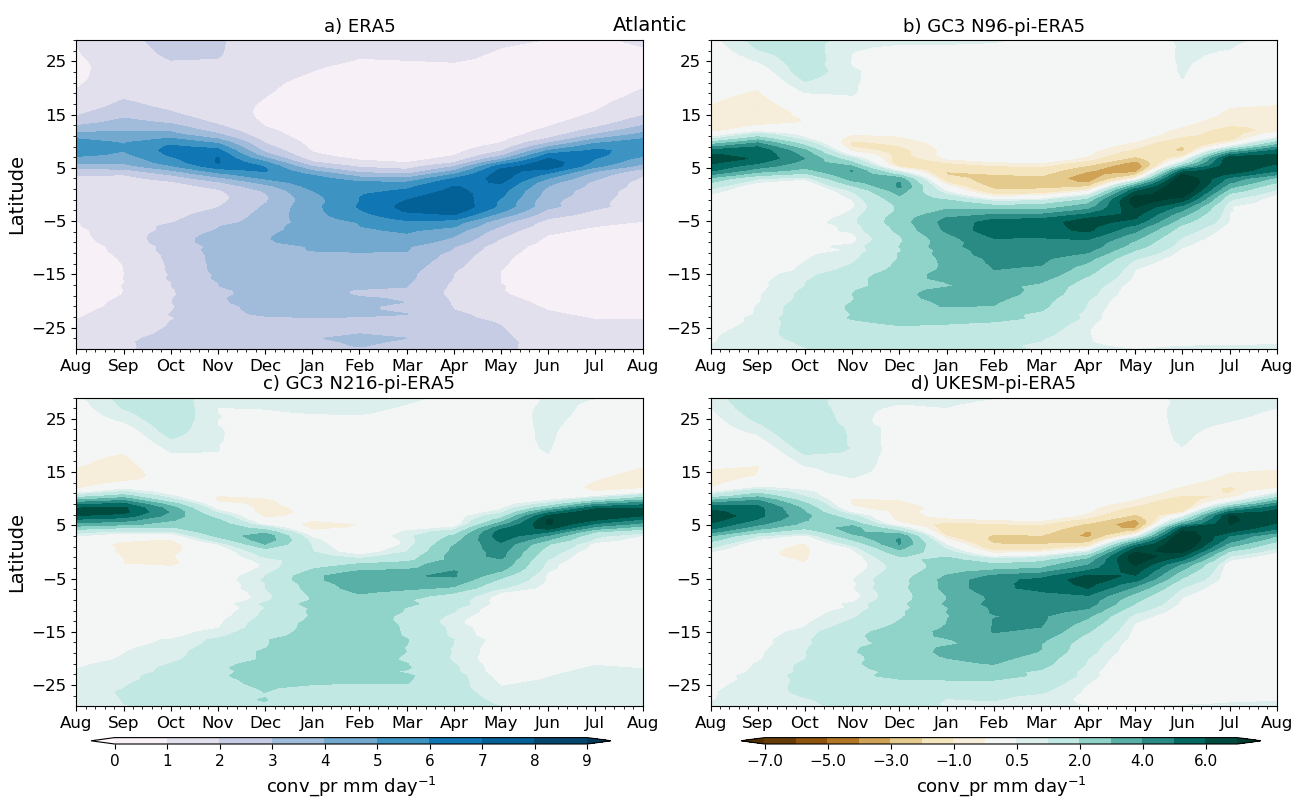
\includegraphics[width=\linewidth]{figures/climcmip_bconv_pratl.png}
\caption[ITCZ seasonal cycle in the Atlantic Sector.]{(a) Monthly and zonal-mean convective precipitation in ERA5 in the Atlantic sector [60$^\circ$W-20$^\circ$W. (b-d) Biases in GC3 N96-pi, GC3 N216-pi and UKESM-pi. }
\label{fig:itczclimatl}
\end{figure}

This section examines more closely changes to the ITCZ position and strength associated with the phase of the QBO, specifically over the Central Pacific and Atlantic sectors. 
Note that the biases in the representation of the ITCZ in these models (characterized in Chapter \ref{ch:4-ams}) are considerable and could mean that the simulated interaction between the QBO and the ITCZ are different in the model than in the real-world. 
For example, Figure \ref{fig:itczclimatl} shows the seasonal march of convective precipitation in the Atlantic sector in ERA5 and the biases in the three simulations with respect to ERA5. The Atlantic ITCZ in these simulations is not well represented, as shown in previous sections, as the models show a southward bias particularly in DJF and overestimates the maximum precipitation rate at the ITCZ location. In the Central Pacific sector (not shown), the models do not show a bias in the position of the ITCZ but rather a bias in the magnitude of convective precipitation, as all the models overestimate the amount of convective precipitation throughout all the seasons. 
 


\begin{figure}[t!]
\centering
 %\noindent
 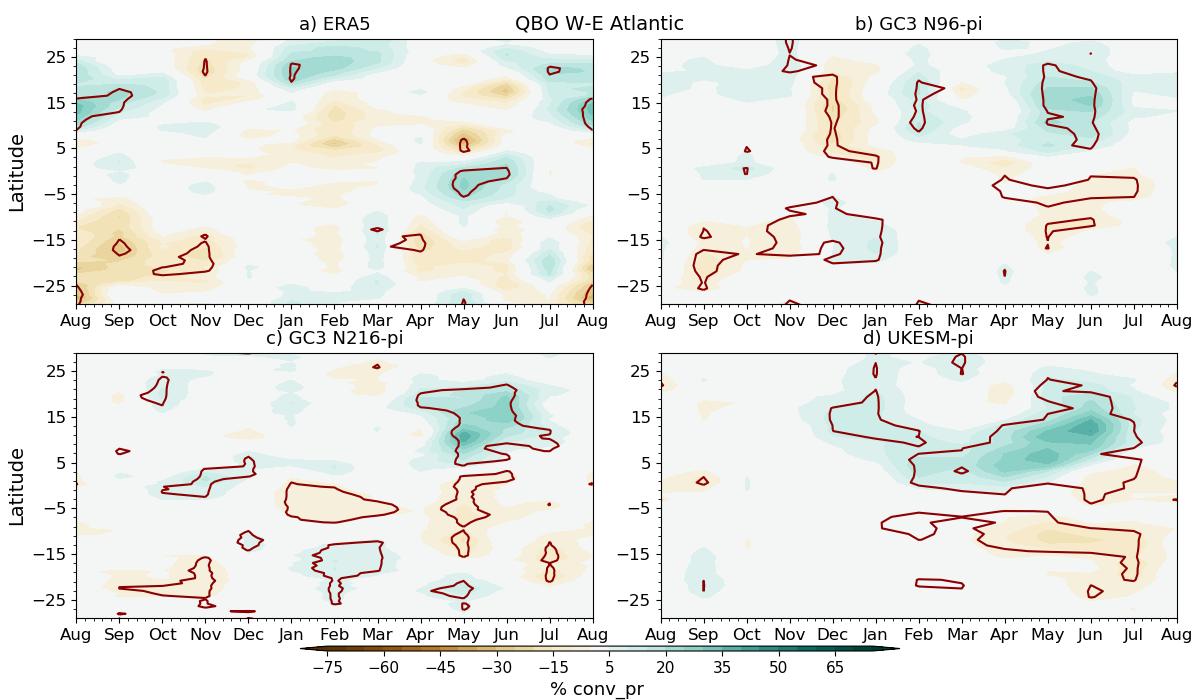
\includegraphics[width=\linewidth]{figures/anomcmip_conv_pratlqbow.png}
\caption[Atlantic ITCZ convective precipitation differences on QBO phase.]{ Zonal mean QBO W-E differences in convective precipitation rates in the Atlantic sector per month, shown as percent (\%) where the difference is weighted by the climatological value at each latitude  and month. The line-contour (red) depict differences that are statistically significant to the 95\% level according to a bootstrapping test. }
\label{fig:itczqbowatl}
\end{figure}


\begin{figure}[t!]
\centering
 %\noindent
 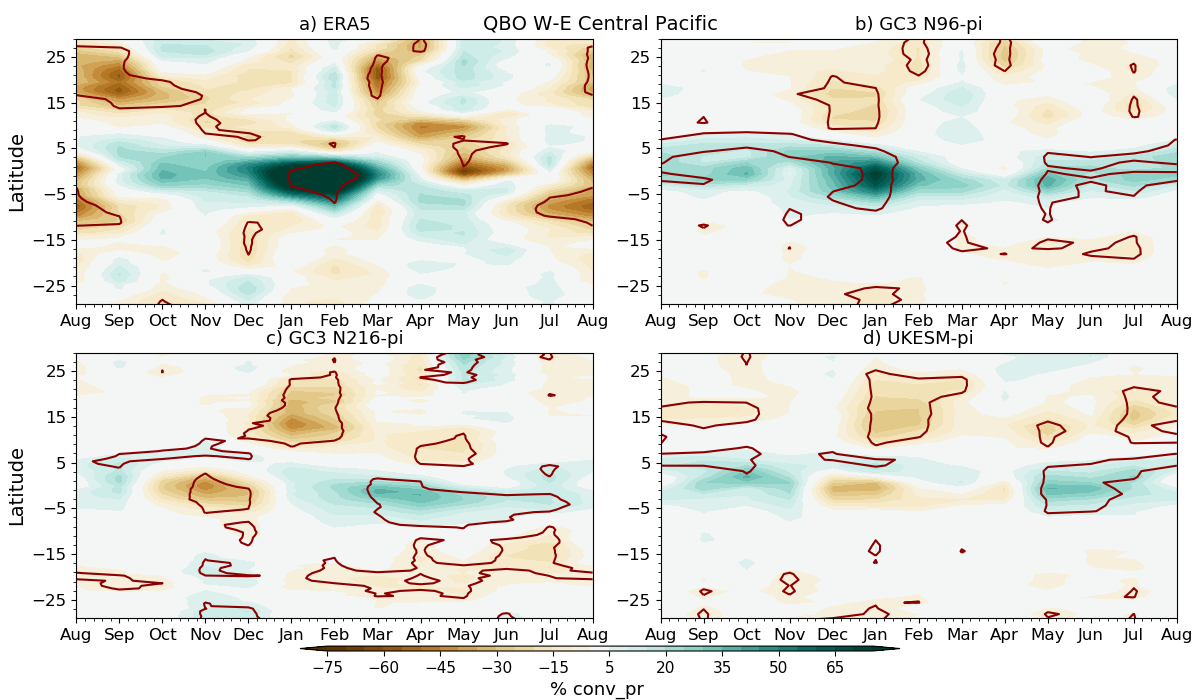
\includegraphics[width=\linewidth]{figures/anomcmip_conv_prcpqbow.png}
\caption[Central Pacific ITCZ convective precipitation differences on QBO phase.]{As in Figure \ref{fig:itczqbowatl} but for the Central Pacific sector [180$^\circ$W-140$^\circ$W.}
\label{fig:itczqbowcp}
\end{figure}

%Any effect that the QBO may have on the Atlantic and Pacific ITCZs will be affected by these biases. 
Figures \ref{fig:itczqbowatl} and \ref{fig:itczqbowcp} show the time-latitude difference in convective precipitation to the phase of the QBO in the Atlantic and Pacific sectors, respectively. 
The northward shift of the ITCZ during QBOW in the Atlantic sector highlighted in previous sections is confirmed in Figure \ref{fig:itczqbowatl}. In all the simulations, but specially in UKESM-pi, there are two significant responses observed from March to July, one wet anomaly north of 5$^\circ$N and a corresponding dry anomaly south of 5$^\circ$S. The southern negative difference is weaker (-20\%) than the positive response north (+40\%). 
The response in ERA5 is relatively less robust, with few significant patterns but this dataset is very short (38 yrs) compared to the long simulations. % the positive response in August-September 

The southward shift of the ITCZ in the Central Pacific, reported in previous observational studies \citep{gray2018}, is confirmed by Figure \ref{fig:itczqbowcp} which shows that in ERA5 a southward shift of the Central Pacific ITCZ is observed in DJF. 
The simulations agree well with this southward shift, particularly GC3 N96-pi during DJF. However, the southward shift response of the Central Pacific ITCZ is also observed in other seasons, for example, from May to September in UKESM-pi and GC3 N96-pi, whereas in GC3 N216-pi the southward shift response is seen from February to July.


These results suggest that the response to the phase of the QBO may depend on the climatological representation of the ITCZ position and strength. Nevertheless, these three simulations which exhibit slightly different representations of the ITCZ as well as of the QBO, agree on the southward shift of the Pacific ITCZ and the northward shift of the Atlantic ITCZ as the main difference between the phases of the QBO. 

\begin{figure}[t!]
\centering
 %\noindent
 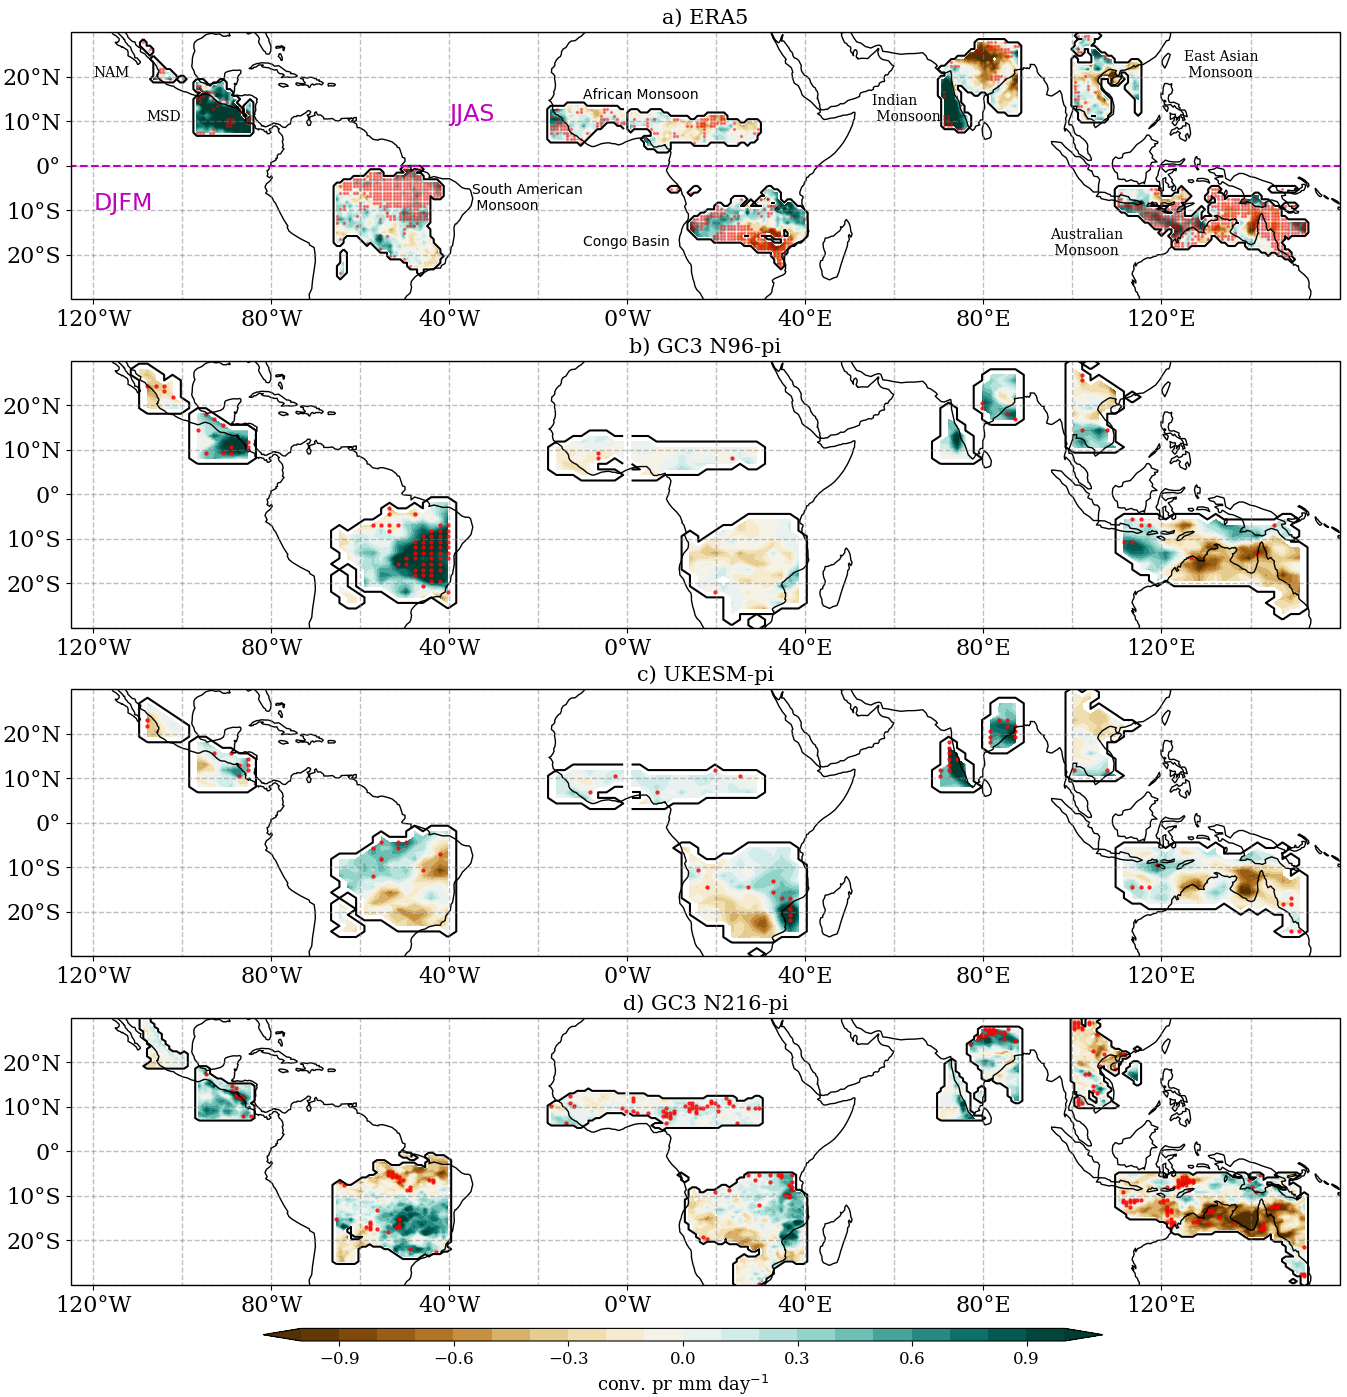
\includegraphics[width=\linewidth]{figures/monsoon_cmip_qbownn.png}
\caption[Global monsoon impacts of the QBO.]{ Convective precipitation differences in monsoon regions between QBO W-E  phases during Neutral ENSO months for a) ERA5, b) GC3 N96-pi, c) UKESM-pi and d) GC3 N216-pi. For monsoon regions in the Northern hemisphere, differences are shown for the JJAS period, whereas for Southern Hemisphere monsoons, results are shown for DJFM.  Red dots indicate differences that are statistically significant to the 95\% level according to the bootstrapping test.}
\label{fig:mons_map}
\end{figure}

In spite of the multiple lines of evidence that suggest a modulation of the QBO over convective activity in land monsoon regions, the results in the previous section show little-to-no effect of the QBO on precipitation over land in these simulations. 
In order to investigate the precipitation response over land more closely, the global monsoon regions are defined within each simulation.  A monsoon region is defined as where over 55\% of the total annual rainfall is observed or simulated in the respective summer season and the summer-winter rainfall rate difference is higher than  2 mm day$^{-1}$\citep{wang2008,wang2017,wang2021monsoons}. 

The local summer convective precipitation differences between QBO phases in monsoon regions (Figure \ref{fig:mons_map}) shows that there is no region where a clear, robust and region-wide effect is observed, even when the influence of ENSO is removed by considering months where ENSO was in a neutral state. Monsoon regions like the Congo Basin, the East Asian and Australian monsoons show both positive and negative responses within the domain of their regions, suggesting a rather heterogenous response, and perhaps suggest that the QBO effect over a monsoon region is also modulated by the dynamics of the regional monsoon. 

%The regions where the response is significant is also sparse within each monsoon region. 

\begin{figure}[b!]
\centering
 %\noindent
 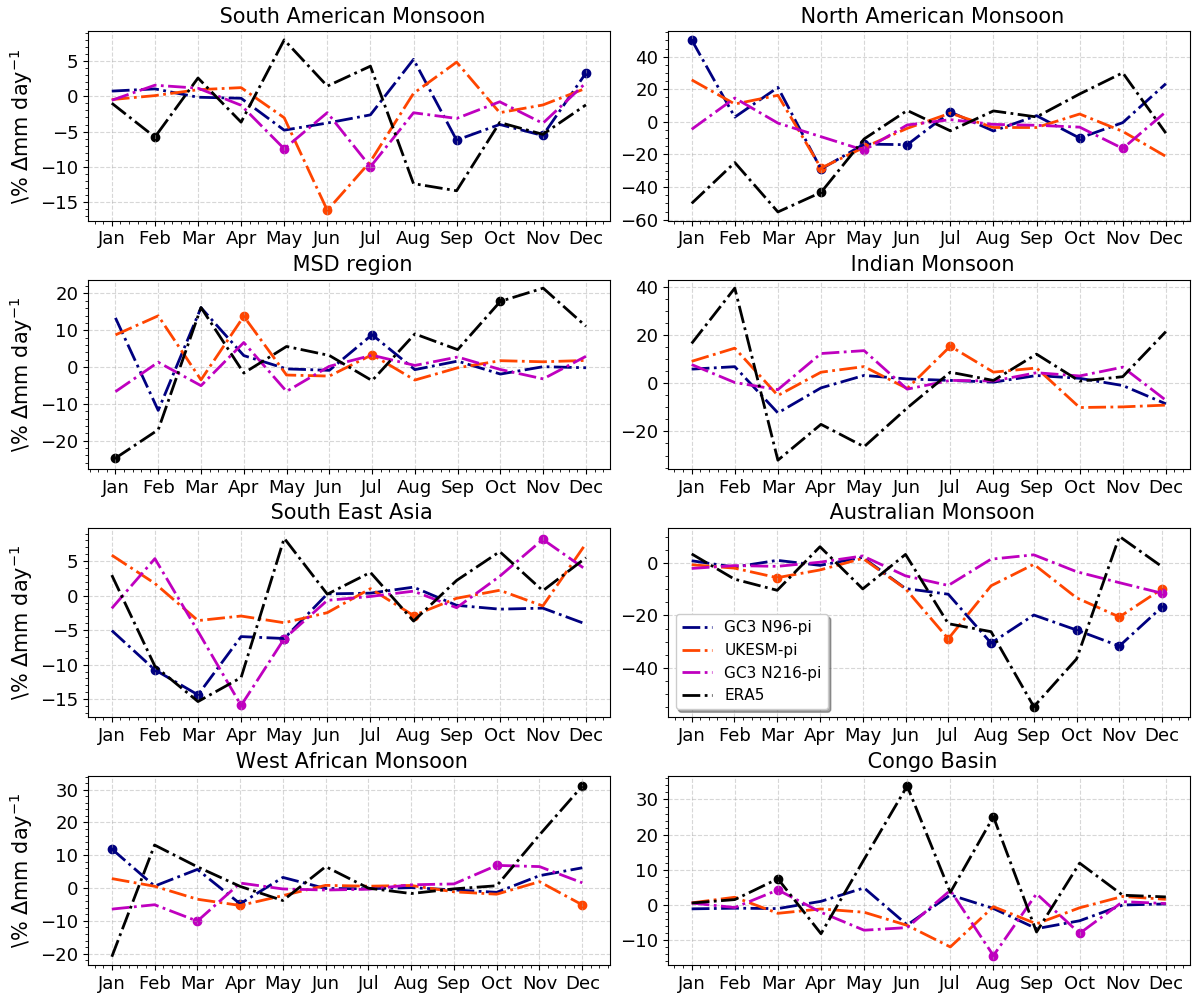
\includegraphics[width=\linewidth]{figures/mons_init_conv_prcompari.png}
\caption[Impacts of the QBO in the seasonal cycle of monsoon regions.]{QBO W-E difference in convective precipitation in monsoon regions separated per calendar month. Dots overlaying lines indicate differences that are statistically significant to the 95\% level according to the bootstrapping test.}
\label{fig:mons_convpr}
\end{figure}

However, some features appear to be robust, as some differences are significant in all three simulations. For example, a positive response is observed in the MSD and northern Indian monsoon regions and a dry anomaly is seen over the Australian monsoon, although the latter is only widely significant in GC3 N216-pi. 
In the South American monsoon region, a dipole of wet and dry anomalies are observed in UKESM-pi and GC3 N216-pi, but these two simulations show an opposite pattern. 
The impacts over the southeastern coast of Brazil in all the three simulations may suggest an effect over the South Atlantic Convergence Zone, which may further modify the dynamics of the monsoon. 
The implication of these results is that feedbacks with the dynamics of the monsoons may be more important than the effects of the QBO over the mass flux and convective activity at the grid-point scale. 



To understand the temporal variability of these effects, Figure \ref{fig:mons_convpr} shows the difference in area-averaged convective precipitation between QBO phases for monsoon regions for each calendar month. There is no clear signal of the QBO over any monsoon region for a large part of the year. For example, all three simulations agree in a negative QBO W-E difference in the Australian monsoon region for November and December, and this response is significant; however, the response in Jan-Mar is weak and not significant. This means that the effect of the QBO over the Australian monsoon region is found only in the early local summer season.

 Similarly, over the Mesoamerican MSD region, all three simulations agree on a wet anomaly during the local summer, but this response is constrained to the month of July (the drier period of the rainy season) and is only significant in two out of the three simulations. 
 In the Indian Monsoon region, UKESM-pi shows a significant wet anomaly, in agreement with the seasonal mean results found in the previous section, however, the other models show a weak and not significant difference. 
Significant relationships are found for other monsoon regions in specific months but no consistent relationship is found in any monsoon region across all three models, which agrees with the lack of robust seasonal-mean patterns presented in the previous section. 


%The three simulations 



\subsection{ENSO, the IOD and the Walker circulation}



The previous section showed that the strongest precipitation responses to the QBO phase in the tropics are found in the Pacific and Indian Oceans, regions that are connected through the overturning Walker circulation and ENSO teleconnections \citep{cai2019pantropical}. For that reason, this section investigates more closely the variability of the Indian Ocean, ENSO events and the Walker circulation associated with the QBO.

The Indian Ocean Dipole (IOD) is a coupled ocean-atmosphere feature of the tropical Indian Ocean characterized by a zonal gradient of SSTs that peaks in boreal fall \citep{saji1999iod,wang2014iod,mckenna2020iod}. IOD events are affected by ENSO events but  the IOD  can also have independent long-distance effects through the Walker circulation \citep{wang2014iod}. The previous section showed a zonal gradient in the precipitation response to the QBO, particularly during boreal fall (SON) (Fig. \ref{fig:qboson}). %However, in these models there was no significant SST response during this to the canonical IOD definition.

\begin{figure}[t!]
\centering
 \noindent
 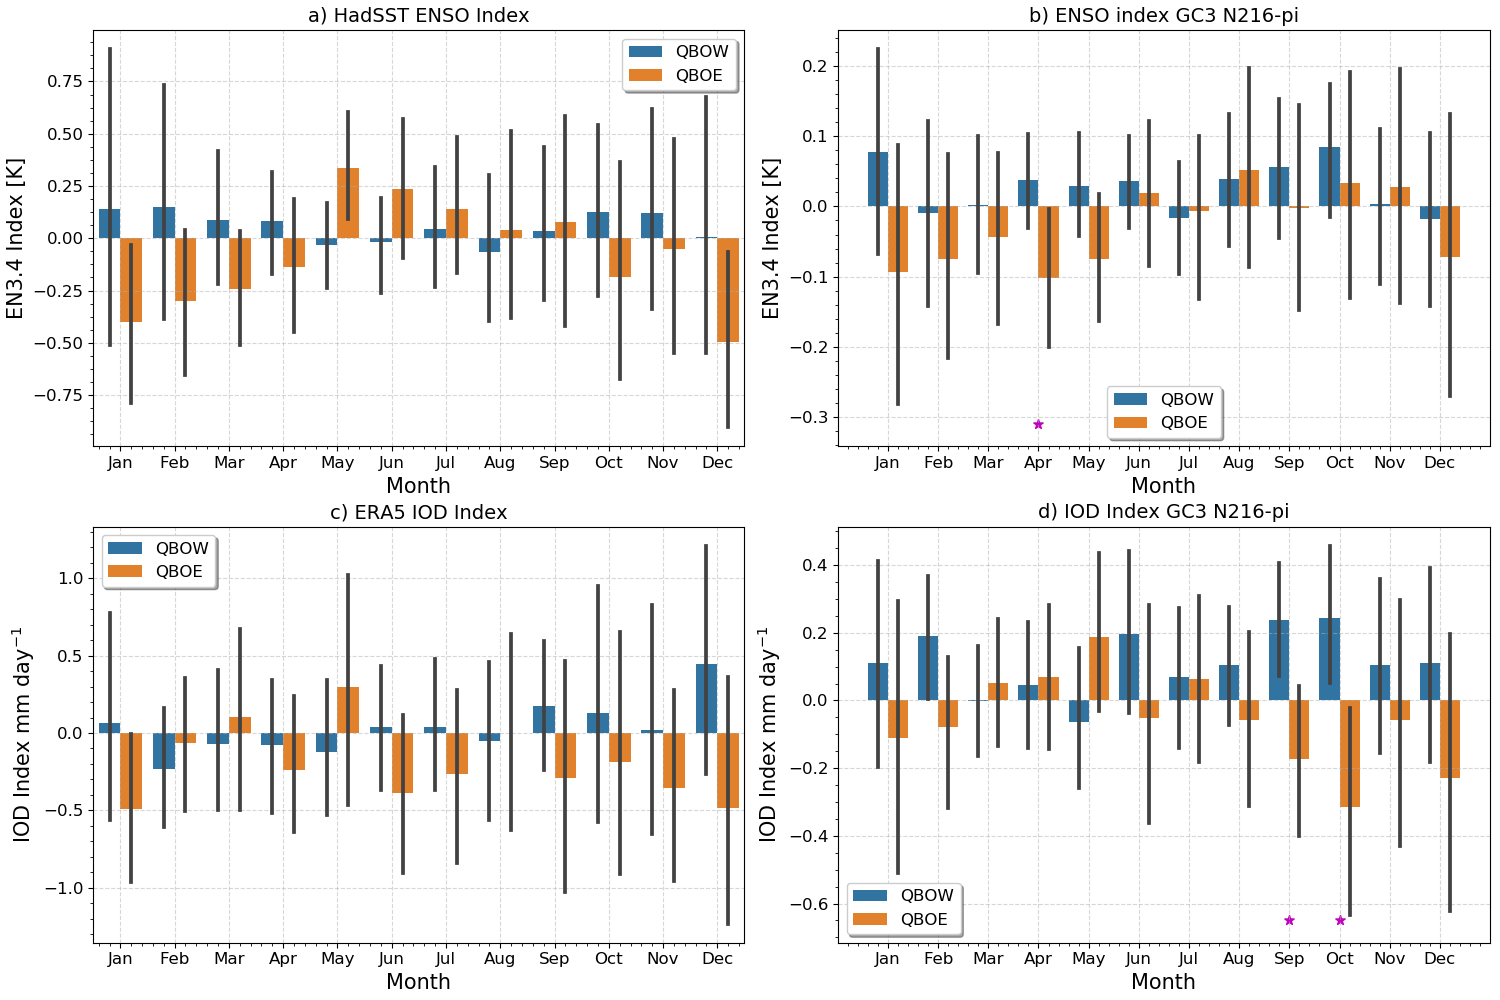
\includegraphics[width=\linewidth]{figures/iod_barplot.png}
\caption[IOD and ENSO frequency changes on QBO phase.]{ Monthly-mean (a) IOD-prc and (b) EN3.4 index separated per QBO phase in GC3 N96-pi. \added{(c,d) Bar plots of the frequency of event ocurrence for each model for (c) positive and negative IOD events based on the convective precipitation index and for (d)  El Niño (EN) and La Niña (LN)  events}. In c,d the count of events in each QBO phase is normalized per total months in each QBO phase so there is no effect associated with an uneven frequency of QBOW versus QBOE events. The error bar show the 95\% confidence interval using a distribution obtained using bootstrapping test where 36 year periods were sampled from the entire run period  10,000 times  and N216 and N96 labels refer to GC3 N216-pi and GC3 N96-pi, respectively.}
\label{fig:iod_barplot}
\end{figure}

The computation of the standard IOD index, a measure of the SST gradient between the western tropical Indian Ocean and the Java-Sumatra region, results in little-to-no correlation with the QBO phase and IOD events defined using this index showed the same frequency under QBOW than during QBOE (not shown). 
Alternatively, a convective precipitation index of the zonal gradient in the Indian Ocean (convective IOD Index), can be defined as the difference of the deseasonalized area-averaged convective precipitation between the western [50-70$^\circ$E] and eastern [80-100$^\circ$E] equatorial [10$^\circ$S-10$^\circ$N]. 
Using this convective precipitation index, IOD events are defined as in previous studies using a 1 standard deviation to define positive and negative events. 

The relationships between the mean ENSO and convective IOD indices, as well as the frequency of ENSO and IOD events, and the phase of the QBO are significant for all the experiments (Figure \ref{fig:iod_barplot}). 
The mean IOD Index and the EN3.4 SST index in GC3 N96-pi are significantly different depending on the QBO phase in GC3 N96-pi. In particular, the mean IOD Index is positive in QBOW and negative in QBOE months from September until January. The EN3.4 index also shows a non-zero mean when separated by QBO phase, with positive mean values found during QBOW and negative values during QBOE. 
The GC3 N216-pi and UKESM-pi results are very similar (not shown) and the differences are also significant; the only notable difference is the month in which the strongest response in each model is observed for each index. 
In observations, more El Niño events have been noted to occur in QBOW conditions \citep{christiansen2016}, whereas relationships have also been documented between the tropospheric quasi-biennial oscillation (TBO), and the IOD and ENSO \citep[e.g.][]{pillai2010}.

The frequency of El Niño (EN) and La Niña (LN) months is robustly linked to the QBO phase in the three simulations (Fig. \ref{fig:iod_barplot}c). 
EN months are more frequent during QBOW phases than during QBOE phases, and in contrast, more LN events are diagnosed during QBOE than during QBOW. 
Similarly, the number of IOD+ events is increased in the westerly phase of the QBO, whereas negative event frequency is increased during QBOE (Fig. \ref{fig:iod_barplot}d) for all the three models. 
The confidence interval in Fig.  \ref{fig:iod_barplot}c-d  is provided by a bootstrapping test sampling the simulations into 36 yr samples and suggest that this result is robust to internal variability within the model. 


In addition, several tests were done to evaluate whether changes in the frequency of IOD events were associated with known connections between the IOD and ENSO. 
Results show that the changes to the frequency of IOD events remain unchanged when only Neutral ENSO months are considered so there is no aliasing with the influence of ENSO on the IOD. Similarly, these changes in the frequency of IOD events are seen in the three simulations in each month from September to January, so there is no aliasing of the seasonality of the QBO within the model and the seasonality of IOD events. 
Note that these results do no providence any evidence of cause and effect between the QBO and IOD and ENSO indices and only evaluate the nature of these relationships within the model.

\begin{figure}[t!]
\centering
 \noindent
 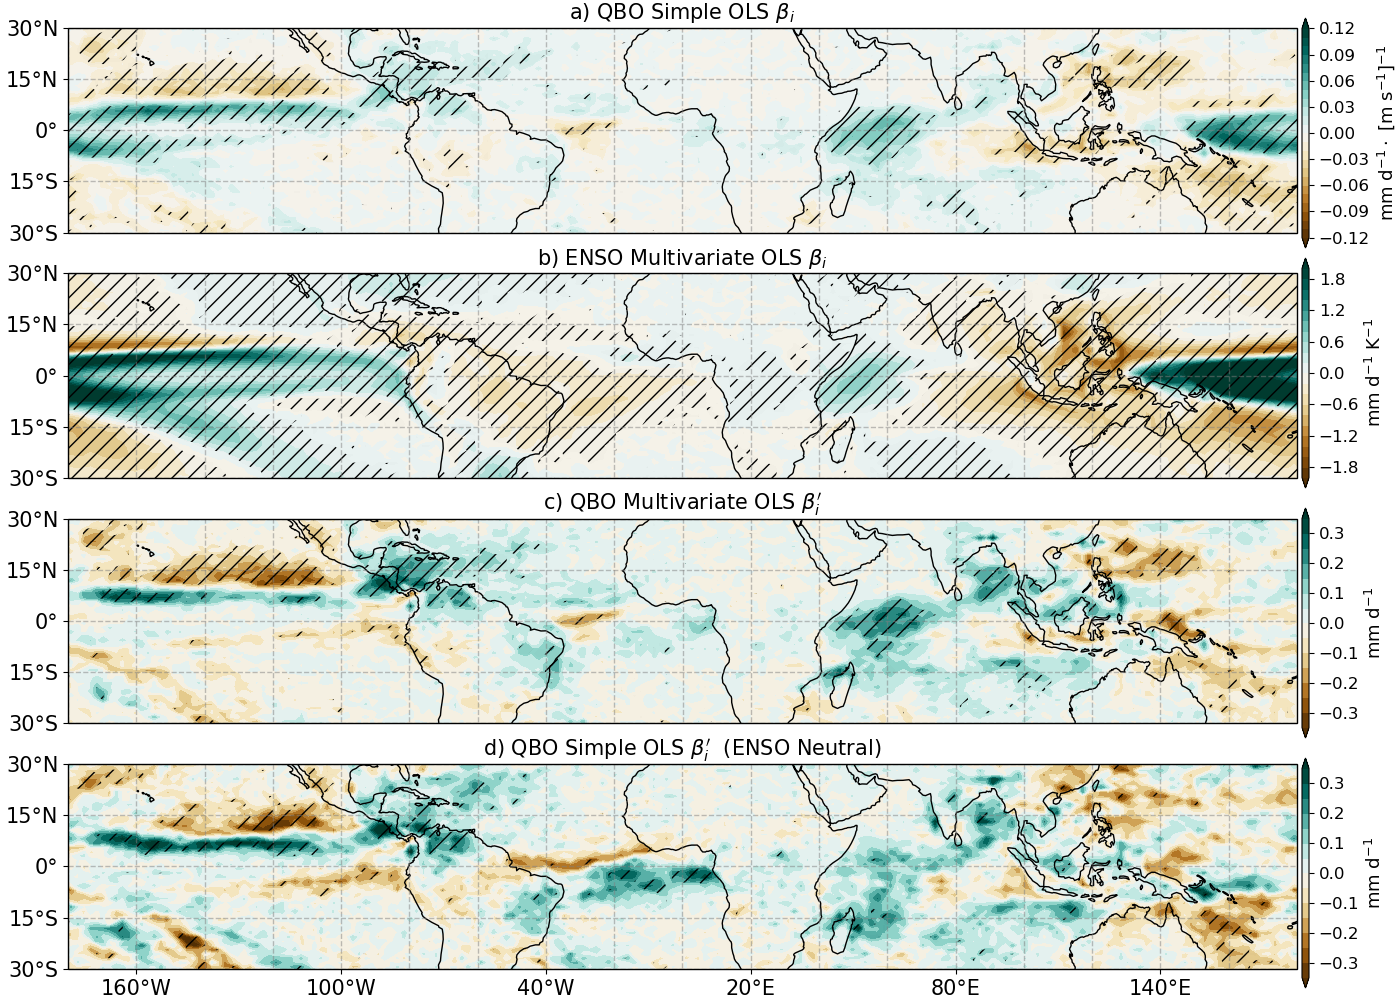
\includegraphics[width=\linewidth]{figures/regress_gc3.png}
\caption[Convective precipitation regression analysis]{Regression model results in GC3 N96-pi. (a) Regression coefficients ($\beta_i$) from a simple ordinary least-squares (OLS) regression model with the QBO index, (b, c) the regression coefficients resulting from a multivariate regression model using the ENSO and QBO indices for the (b) ENSO and (c) QBO predictors. In (c) the regression coefficients are rescaled by multiplying the regression coefficients with the ratio of maximum amplitude and standard deviation of the QBO index. (d) Rescaled regression coefficients from a simple OLS model with the QBO index, but using time-series where ENSO was classified as in a Neutral state using the EN3.4 index.  }
\label{fig:enso_regress}
\end{figure}


The previous results showed that there is an uneven frequency of ENSO events in the different QBO phases and that within these experiments, the QBO impacts may depend on the phase of ENSO. 
Linear-regression analysis was used by \cite{gray2018} to investigate the spatial and temporal variability of the surface impacts of the QBO in tropical precipitation using a multivariate-regression model that accounts for the relationship between ENSO and precipitation. 
For these reasons, simple and multivariate regression analysis has been performed using the EN3.4 SST index, the 70 hPa zonal wind QBO index and deseasonalized convective precipitation. Other indices such as solar, volcanic and greenhouse forcings are omitted in this analysis because in these runs external forcings are constant.

Figure \ref{fig:enso_regress} shows results from the regression analysis of GC3 N96-pi. 
A simple regression model using the QBO 70 hPa index (Fig. \ref{fig:enso_regress}a) shows very similar results to the composite mean differences described in the previous section.
The results from the multivariate regression model implemented using the QBO and ENSO indices, show that the spatial distribution of significant regression coefficients for the EN3.4 time-series (Fig. \ref{fig:enso_regress}b) is somewhat similar to results for the QBO in the simple regression model, suggesting the possibility of aliasing between ENSO and QBO indices. 

 The rescaled regression coefficients for the QBO, obtained using the multivariate regression model (Fig. \ref{fig:enso_regress}c), i.e., the model where the influence of ENSO has been regressed-out, are broadly similar to the simple OLS model, except in the equatorial west Pacific. These regression coefficients suggest that the precipitation response of the QBO is a southward shift of the East Pacific ITCZ, as well as a wetter Caribbean Sea and western Indian Ocean for QBOW phases.
 A simple regression model using the QBO index during Neutral ENSO months (Figure \ref{fig:enso_regress}d) shows very similar results, except in the Atlantic ITCZ region, confirming that the influence of ENSO needs to be closely examined and removed before analysing the influence of the QBO over the tropics. 
 
 \begin{figure}[b!]
\centering
 %\noindent
 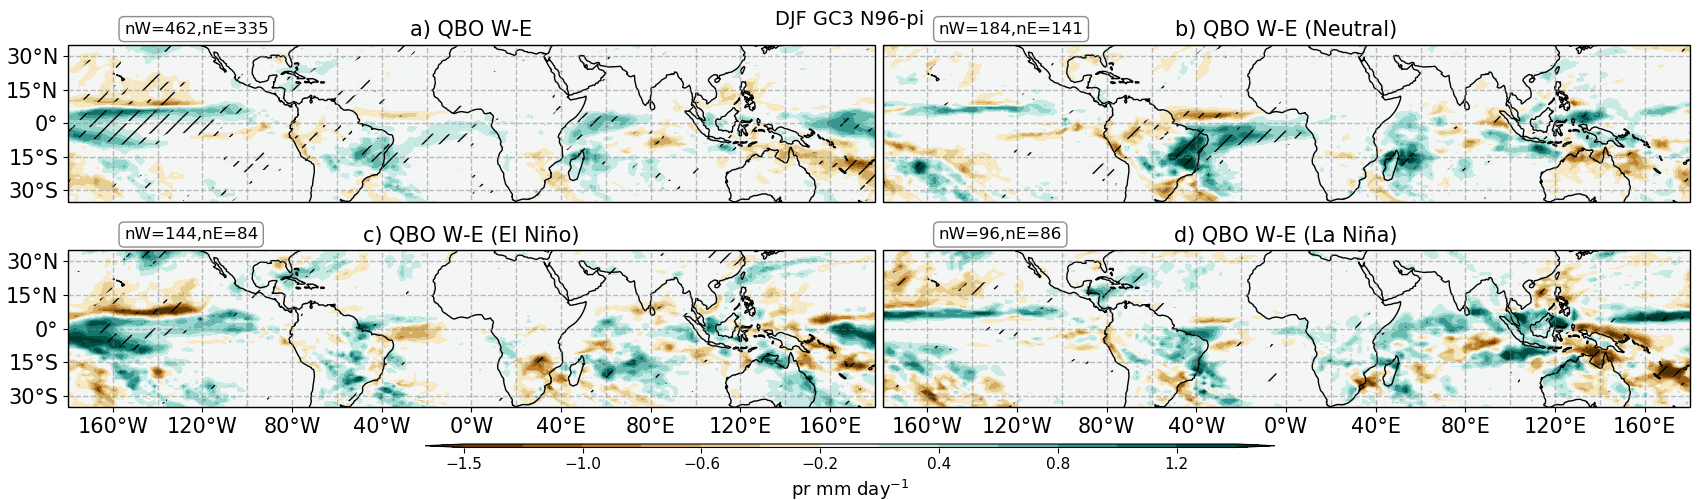
\includegraphics[width=\linewidth]{figures/ensoqboprdjf.png}
\caption[Precipitation response to QBO W-E for GC3 N96-pi under different QBO phases.]{ DJF QBO W-E precipitation differences in GC3 N96-pi for (a) all the events, (b) Neutral ENSO conditions only, (c) El Niño and (d) La Niña conditions. The sample size of each composite is noted in the top left corner of each panel. }
\label{fig:qboenso}
\end{figure}


% Results in GC3 N96-pi, UKESM-pi and GC3 N216-pi showed that the spatial distribution of the coefficients from the simple regression model varied notably if the time-series selected for La Niña, El Niño or Neutral states-only. In particular, the equatorial Atlantic region showed the strongest sensitivity to the phase of ENSO and QBO. 
 %These results suggest a non-linear non-symmetric interaction between the QBO and the ENSO for impacts to the Atlantic Ocean. However, these impacts may be too weak to disentangle these relationships from ENSO within these simulations.
 %The next section describes new modelling experiments that aim to address these questions by improving the signal of the QBO within the MOHC model. 

The seasonal-mean  results could possibly be aliasing effects of ENSO and the regression results have removed the influence of ENSO. A different question, however, is whether the QBO could modify the teleconnections of ENSO in the tropics. An analysis of the DJF mean response to phase of the QBO separated also by ENSO phase (Figure \ref{fig:qboenso}) shows that the surface response depends on both the QBO and ENSO phase. % could modify the seasonal mean results and the extent to which regression analysis is appropiate is analysed, at a first glance, in  which evaluates the DJF mean response to the QBO under different ENSO conditions.

The wet anomaly pattern in the southern equatorial (15$^\circ$S-O$^\circ$) Central Pacific observed in the mean DJF response is only observed during during El Niño events, not during Neutral or La Niña months. In turn, the dry anomaly in the Central Pacific at 10$^\circ$N-20$^\circ$N is observed during both la Niña and El Niño seasons but not during Neutral conditions.
 Over the Atlantic ITCZ region and eastern Brazil, the strongest response is observed during Neutral conditions, suggesting that the pattern observed in panel a) is likely the closest to a true QBO response independent from ENSO and that this response is characterized by a southward shift of the ITCZ during QBOW. 

Similar results are found other seasons (MAM and SON) and simulations, which confirms that within these simulations the ENSO teleconnections can depend on the QBO phase.
One implication of these results may be that ENSO teleconnections are themselves a function of the QBO state and that the impact of the QBO may be different for La Niña than for El Niño, an effect that would be masked by the regression analysis presented above. 

\begin{figure}[b!]
\centering
 \noindent
 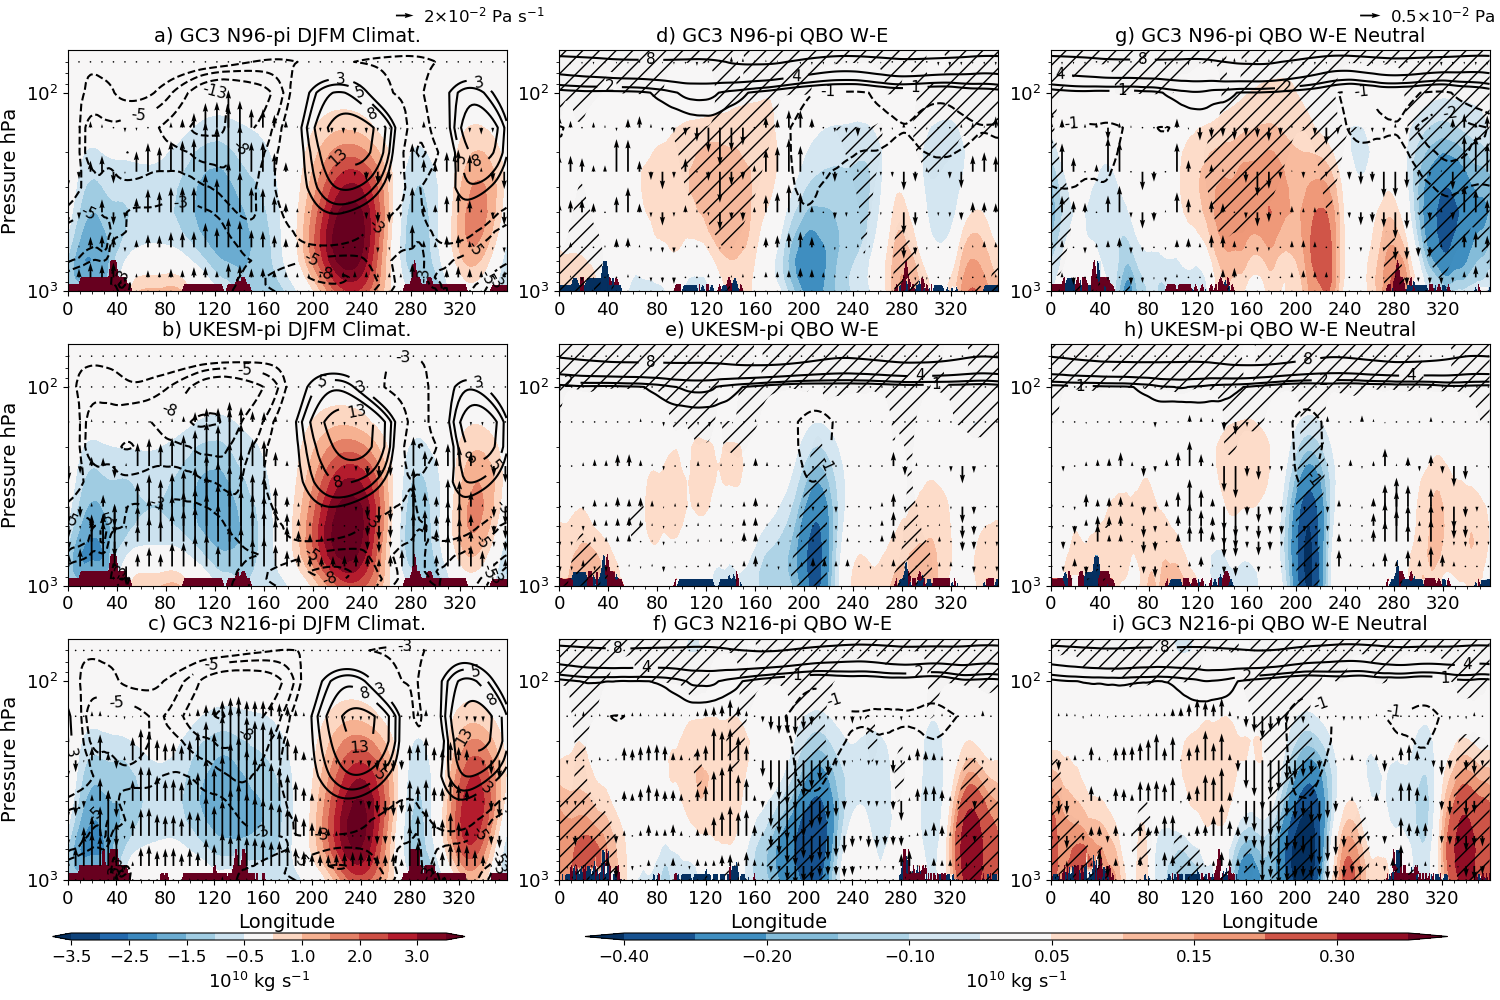
\includegraphics[width=\linewidth]{figures/cmip_streamdjfm.png}
\caption[Walker circulation anomalies in DJFM]{(a-c) Climatological mean-state of the Walker circulation, depicted through the zonal streamfunction ($\psi$) in shading, the zonal wind (contours), and vertical velocity ($\omega$ [Pa s$^{-1}$], vectors) during the DJFM season in the three simulations. (d-f) show W-E composite differences, during DJFM, for the same variables only that hatching represents statistical significance to the 95\% confidence level for differences in the streamfunction, and only statistically significnat differences in the zonal wind and $\omega$ are shown. (g-h) are as in (d-f) but considering Neutral ENSO periods only. Example vector for $\omega$ are given in the top right corners of a and g.  }
\label{fig:walker_djfm}
\end{figure}

Results in Chapter \ref{ch:4-ams} and in this chapter suggest a link between QBO, ENSO and the Walker circulation. For that reason, an analysis of the zonal streamfunction, zonal wind and vertical velocity in the deep tropics is now presented to better characterise whether the QBO has any possible influence on the mean-state and variability of the zonal overturning in the tropics. 
The zonal streamfunction \citep{yu2010,bayr2014} is defined as:

\begin{equation}
\psi=2\pi \frac{a}{g} \int_0^p u_D dp,
\end{equation}

\noindent where $\psi$ is the zonal streamfunction, $u_D$ is the divergence part of the zonal wind, $a$ is the Earth's radius, $p$ is the pressure coordinate and $g$ the gravitational constant.
The streamfunction is calculated by first averaging in the equatorial band of 10$^\circ$S-10$^\circ$N and integrated to the top level within the model. 



Results in previous sections show that the boreal winter and early spring exhibit the strongest responses in the Pacific region and in boreal fall in the Indian Ocean. For that reason, the QBO response of the Walker circulation is illustrated for DFJM and SON in Figures \ref{fig:walker_djfm} and \ref{fig:walker_son}.
The streamfunction mean values are higher in DJFM than in SON, indicative of a stronger Walker circulation during boreal winter.

\begin{figure}[b!]
\centering
 \noindent
 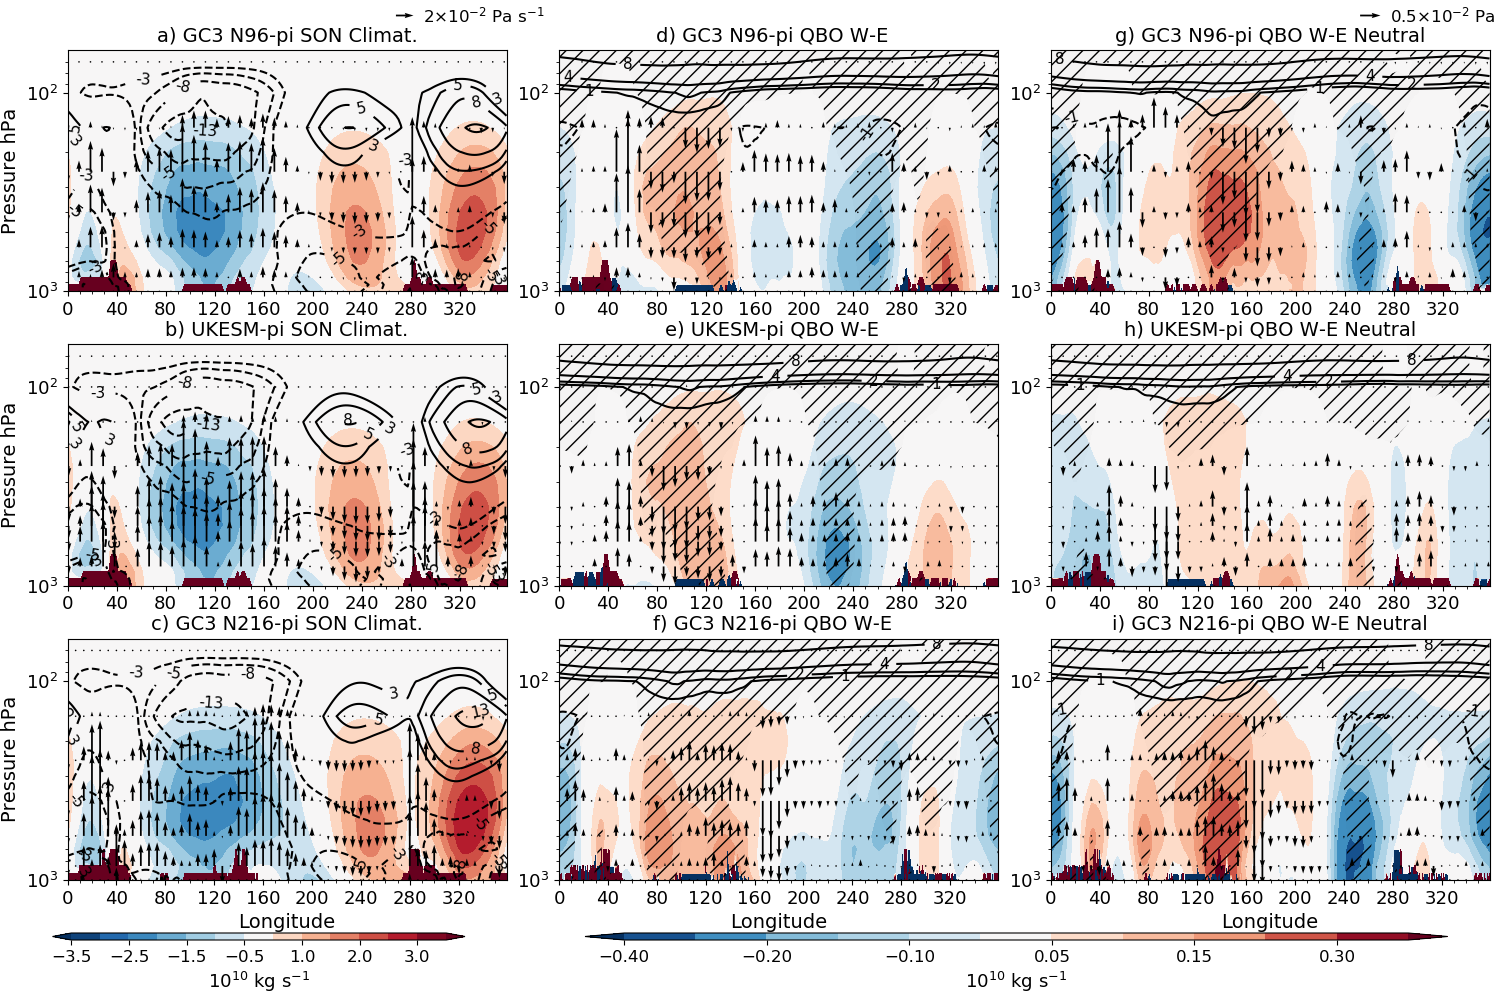
\includegraphics[width=\linewidth]{figures/cmip_streamson.png}
\caption[Walker circulation anomalies in SON]{As in Figure \ref{fig:walker_djfm} but for SON. }
\label{fig:walker_son}
\end{figure}

Composite differences in DJFM show that the streamfunction from 180-240$^\circ$E is significantly weaker during QBOE than during QBOW in all three simulations (Fig. \ref{fig:walker_djfm}). The zonal wind at upper-levels (300-100 hPa) is also weaker during QBOW at 200$^\circ$E. In GC3 N216-pi, this negative $\psi$ difference is accompanied by descending motion anomalies in the 190-220$^\circ$E region, whereas anomalous ascent is observed in the Maritime continent and Indian Ocean. Vertical velocity ($\omega$) anomalies in the other simulations are weaker in the Central-Eastern Pacific. 
These results suggest a weaker Walker circulation during QBOW compared to QBOE seasons. 
The rightmost panels in which only Neutral ENSO months are removed, suggest that this relationship between the QBO and the Walker circulation occurs regardless of ENSO events.
% and, in fact, these composite differences are different when only El Niño or La Niña months are considered (not shown). 

In boreal fall (Fig. \ref{fig:walker_son}), the mean Walker circulation is weaker and ascent is mostly concentrated in the Indian Ocean and Maritime continent, as well as in South America. 
Positive streamfunction differences are found to be significant over the Indian Ocean in all three simulations, associated with anomalous descent on the eastern Indian Ocean and ascent over the western Indian Ocean. These results agree well with the results using convective precipitation index for the IOD, described in the previous section, which found more rainfall in the western Indian Ocean than in the east during QBOW than during QBOE. 

Furthermore, in SON, significant negative differences in the streamfuncion are found in the Eastern Pacific and Atlantic Oceans and positive differences over South America, although in both cases differences in $\omega$ appear very small or not significant. 
These results suggest that there are possible links between ascending and descending motions in the Indian Ocean and the Pacific and Atlantic Oceans through the boreal fall Walker circulation.


\section{Summary and discussion}

This chapter investigates the tropical route of QBO teleconnections in the pre-industrial control experiments of the MOHC from HadGEM3 and UKESM1.
Results in this chapter confirm observational evidence \citep{collimore2003,liess2012,gray2018}  that there is a QBO impact over tropical precipitation, mainly over the tropical ocean in the East Pacific and Atlantic ITCZs.


The position of the East Pacific and Atlantic ITCZs is significantly different between the two phases of the QBO in the three experiments; however, the season of strongest influence varies for each model. 
For example, the southward displacement of the East Pacific ITCZ in QBOW compared to QBOE phases  \citep[as previously reported, e.g., by][]{gray2018} is confirmed but in GC3 N216-pi this shift of the ITCZ is strongest in MAM whereas in GC3 N96-pi the most pronounced shift is in the DJF season. 
The position of the Atlantic ITCZ is found further  northward during QBOW than during QBOE periods in all the simulations; the strongest response is found during late boreal spring and early summer in UKESM-pi. 

%In addition to multiple lines of observational and modelling evidence that suggest an influence of the QBO over tropical convective phenomena, results from Chapter \ref{ch:4-ams} showed that the impact of ENSO on the Walker circulation and associated teleconnections was sensitive to the phase of the QBO in the CMIP6 experiments of the MOHC and this chapter follows up on that evidence. 
%The first part of the chapter analyses CMIP6 experiments that reasonably simulate the QBO features, and the second part of the chapter describes and reports the results of simulations realized with MOHC models in which the equatorial stratosphere was relaxed towards an observed state.
%
% First, the chapter describes the annual and seasonal mean surface response of precipitation to the two phases of the QBO in the CMIP6 pre-industrial control experiments: UKESM-pi, GC3 N96-pi, GC3 N216-pi.  
%Results in the models generally agree with the results documented in observational studies \citep{liess2012,gray2018} and with the observational and reanalysis datasets employed throughout this thesis. In particular, the most robust impacts are observed over the ocean, particularly over two coupled ocean-atmosphere phenomena: the East Pacific and Atlantic ITCZ and the IOD. 

For most land-monsoon regions, little evidence was found of robust impacts on the local summer monsoon precipitation associated with the QBO, in spite of observations from satellite-derived and gridded station data suggesting otherwise \citep{collimore2003,liess2012,gray2018,lee2019}. For example,  the South American monsoon region exhibited different responses in eastern Brazil than in the southernmost part of the monsoon. The surface response over land also varied notably from model to model.
One hypothesis for the lack of a spatially coherent signal over land is the differences in the representation of the monsoon dynamics and feedbacks between the three models UKESM-pi, GC3 N96-pi, GC3 N216-pi that may represent the land-surface processes and moisture transport differently, so that any grid-scale impact of the QBO on the convective profile may produce different dynamic responses in the lower troposphere. 

The influence of the QBO over the Indian and Pacific Oceans was confirmed through multi-variate regression analysis, suggesting an independent effect of the QBO from ENSO in these ocean basins. 
However, the QBO-related differences over the Atlantic and East Pacific ITCZ appear to also depend on the phase of ENSO, suggesting a non-linear interaction between the ITCZs, ENSO and the QBO which may be confounded when using regression analysis.  
 The observed relationship between the QBO and ENSO is confirmed in this chapter in the CMIP6 experiments, as more frequently El Niño events appear during QBOW than during QBOE and the opposite for La Niña. 
 
 A zonal gradient of convective precipitation in the Indian Ocean appeared in all the simulations, and this signal maximised during SON. 
 This zonal gradient was further diagnosed through an index that was found to be significantly sensitive to the QBO  phase, the index was found to be positive during QBOW and negative during QBOE, indicative of wetter conditions in the western Indian Ocean than in the eastern  Indian Ocean during QBOW and the opposite during QBOE. To our knowledge, these results are the first suggestions of a surface impact of the QBO associated with the IOD during SON.
 
Observational evidence has found coupled ocean-atmosphere interactions between the IOD, ENSO and the tropospheric quasi-biennial oscillation (TBO), which is a variation of weak-to-strong monsoons with similar periodicity to the stratospheric QBO \citep{meehl2003,pillai2010}. 
This evidence could possibly explain these modelling results suggesting a link between the QBO, the IOD and ENSO simply by aliasing the QBO with the TBO signal.
However, the period of the QBO in UKESM1 and HadGEM3 is longer than in observations, specifically 37-40 months for UKESM1 and 30-34 months for HadGEM3, which means the aliasing with a TBO in the model is unlikely.

 The zonal asymmetry in the QBO surface impacts in the tropics documented in observations \citep{collimore2003,liess2012,gray2018,lee2019} is also observed within these simulations. 
 Regional effects that depend on the longitude suggest that there is not a clear single effect of the QBO over precipitation, in contrast to early suggestions \citep{gray1984} that in general more precipitation would be observed during one phase of the QBO. 
 This chapter demonstrates that the relationship between the QBO and tropical convection is not likely only relevant at the grid-box scale, but the large and regional scale dynamics in the tropics are very important and thus QBO responses appear zonally asymmetric.
 
 The hypothesis that the QBO may influence the mean-state of the Walker circulation suggested by previous observational studies to explain zonally asymmetric responses \citep[e.g.][]{collimore2003,liess2012} is confirmed as the Walker circulation varies by up to 10\% between QBO phases, even when the effect of ENSO events is taken into account. 
 Specifically, the Walker circulation is found to be weaker during QBOW than during QBOE. In DJF, this anomaly of the overturning circulation in the Pacific is likely linked to the East Pacific ITCZ shifts, and in SON, the changes to the overturning are likely linked to the ascending and descending motions in the Indian Ocean that generate the IOD response documented in this chapter.
 
The relationships found between the QBO, the Walker circulation and ENSO frequency could potentially be causally linked with the QBO variability being the driving mechanism. Changes to the mean state of the Walker circulation are known to modify the frequency of El Niño events and La Niña events. A weaker state of the Walker circulation could more likely trigger an El Niño event during QBOW than during QBOE, and similarly, a stronger Walker circulation during QBOE could more likely trigger a La Niña event, which would be consistent with the results of this chapter. 

 
 The results of this chapter are one of the few analyses of the tropical route of QBO teleconnections within a fully coupled GCM. 
 The length of the pre-industrial control experiments (500 yr) was useful to adequately evaluate the statistical significance of the relationships between the QBO and tropical climate features. 
Furthermore, the fact that most of the impacts diagnosed in this chapter are very similar in the three simulations, despite their differences in resolution and inclusion of Earth System processes provides robustness to the results. Nevertheless, the dynamical core of all the simulations is the same, so the parametrisation schemes such as the convective and gravity-wave scheme are identical. Further work needs to evaluate these relationships in different models from CMIP6.
 
 However, the direction of causality cannot be interpreted from the regression or composite analyses presented in this chapter. For example, the ENSO-QBO relationships could be explained by anomalous tropical wave activity associated with ENSO modifying the downward propagation of the QBO \citep{schirber2015} or alternatively, the QBO temperature variability affecting convection in various regions and modifying the tropical circulation. 
Further experiments are needed to separate the mechanisms that could explain these relationships and that could separate the directions of influence between the tropical stratosphere and troposphere. 
 
 % however the direction of causality could not be addressed in this part of the chapter, which leads into the second part of the chapter.
 
 %\end{document}


%\section{The case for nudging}
%
%
%
%Global climate models exhibit a number of biases in their representation of various aspects of the climate, all of which lead to uncertainty in our ability to make statements about the real-world based on their results. One example of a key bias discussed in this thesis is the magnitude and position of precipitation associated with the ITCZ in the Atlantic Ocean, which is associated with biases in South American precipitation. % the mean state of the Pacific and Atlantic SSTs as well as many others. 
%For this section, one relevant bias to consider is how current models represent the tropical stratosphere and, in particular, their representation of the QBO.
%
%
%
%
%The number of GCMs with a full stratosphere have increased notably from CMIP3 to CMIP6 which means that features such as the QBO are increasingly better resolved with each iteration of the CMIP \citep{bushell2020,richter2020}. Nevertheless, several aspects of the QBO are still not well represented by state-of-the-art climate models, such as the period and amplitude of the QBO \citep{schenzinger2017,richter2020}. 
%These biases increase uncertainty in teleconnections diagnosed from these models, because these biases could make the models misrepresent processes that are observed in the real-world between the tropical stratosphere and troposphere.
%
%\begin{figure}[t!]
%\centering
% \noindent
% 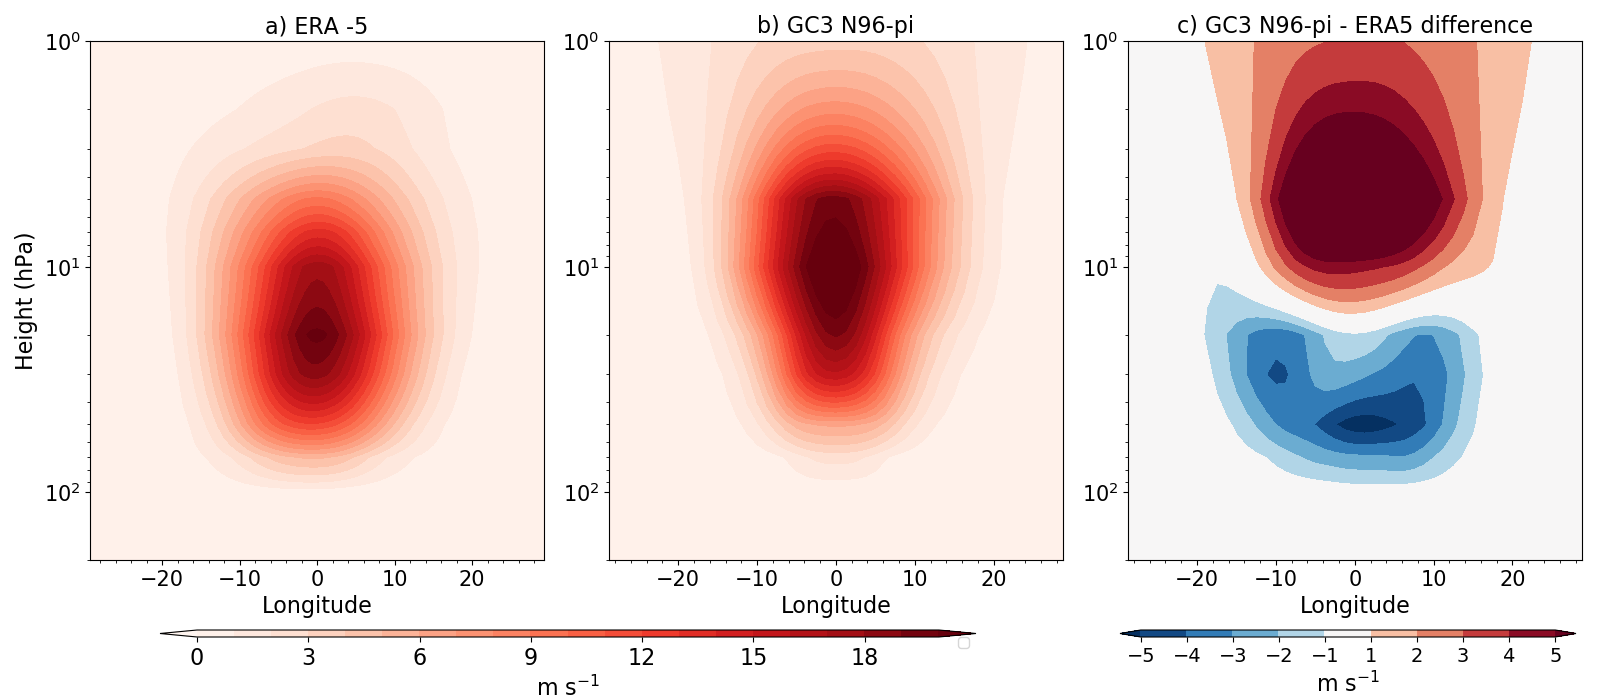
\includegraphics[width=\linewidth]{figures/qboamplitude.png}
%\caption[QBO amplitude bias]{Latitude-pressure plot of the amplitude [m s$^{-1}$] of the QBO. Obtained from the zonal mean zonal wind fourier spectrum magnitude within the QBO periods, as in \cite{schenzinger2017}. }
%\label{fig:qboamplitude}
%\end{figure}
%
%
%
%\section{ Results from nudging experiments}
%
%This section investigates the effect of nudging for the representation of the QBO, the variability in the upper troposphere lower stratosphere (UTLS) associated with the QBO, and ultimately, surface impacts driven by QBO effects on tropical convection. 
%First, this section evaluates how nudging modifies the wind and temperature variability in the UTLS region compared to control and CMIP6 simulations.  
%
%\begin{figure}[b!]
%\centering
% \noindent
% 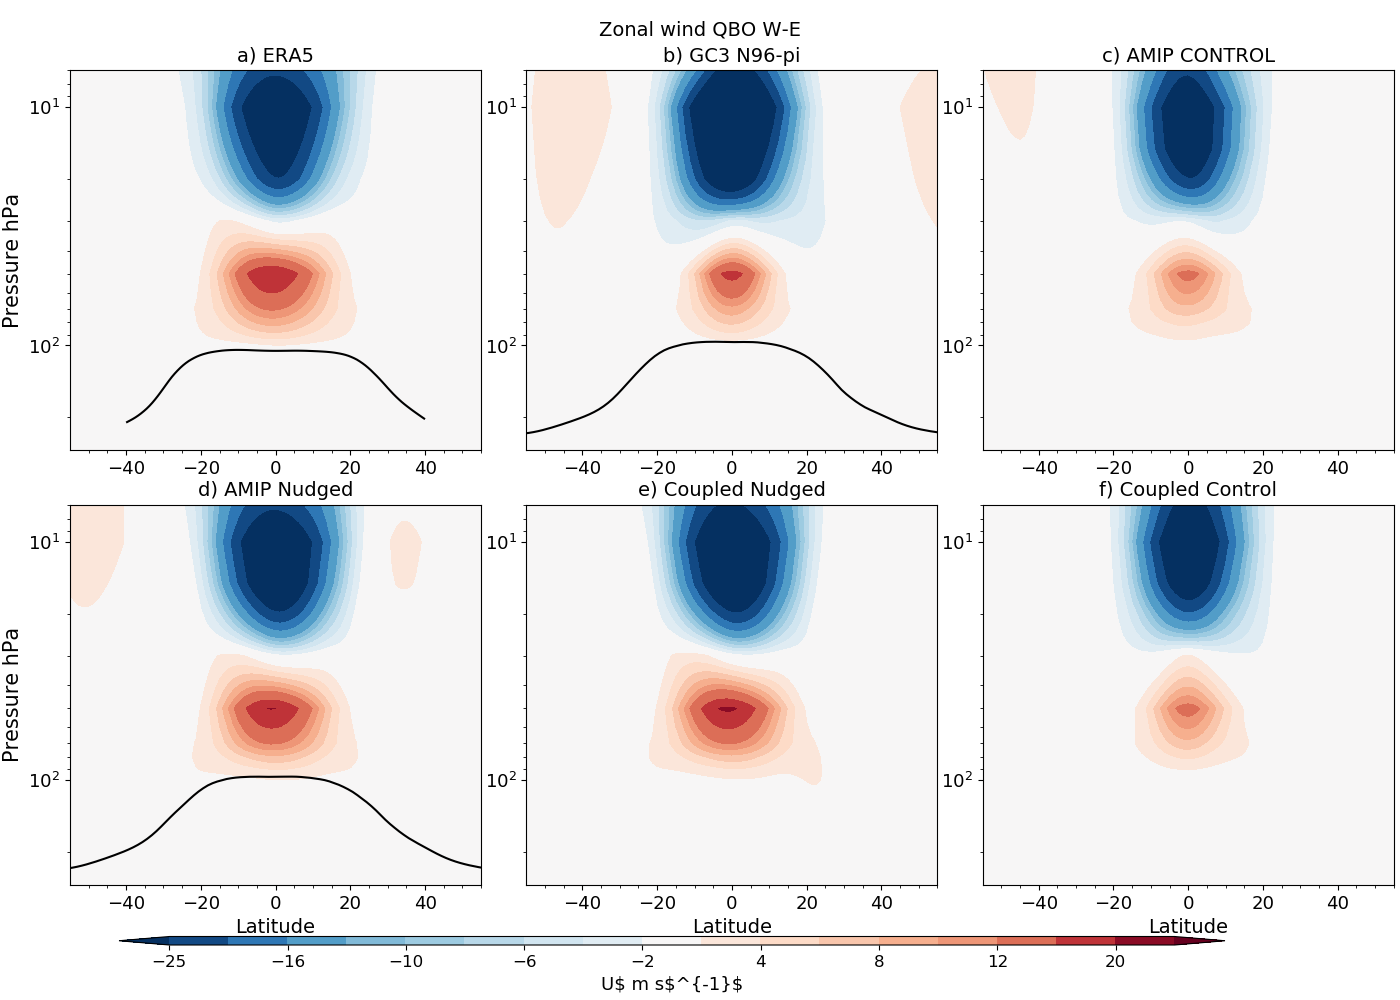
\includegraphics[width=\linewidth]{figures/zonalplotx_wind.png}
%\caption[Zonal mean zonal wind QBO difference]{Latitude-height plot of the zonal-mean zonal wind differences (QBO W-E) in (a) ERA5, (b) GC3 N96-pi from CMIP6, the control simulations with no nuding in an (c) AMIP and (f) coupled configurations, and the nudged simulations in (d) AMIP and (e) coupled configurations. The black line denotes the tropopause height obtained from the model data in (b, d) and for ERA5 the tropopause height was found through the gradient threshold method. For the nudged experiments, the ensemble-mean is shown. }
%\label{fig:zonal_u}
%\end{figure}
%
%
%\subsection{Tropical UTLS variability}
%
%
%Figure \ref{fig:zonal_u} shows that the zonal mean difference in zonal wind associated with the QBO phase, in a latitude-height sense, is deficient in the GC3 N96-pi and control experiments, principally near the tropopause as the signal is too narrow and weaker than in the reanalysis.
% 
%\begin{figure}[b!]
%\centering
% \noindent
% 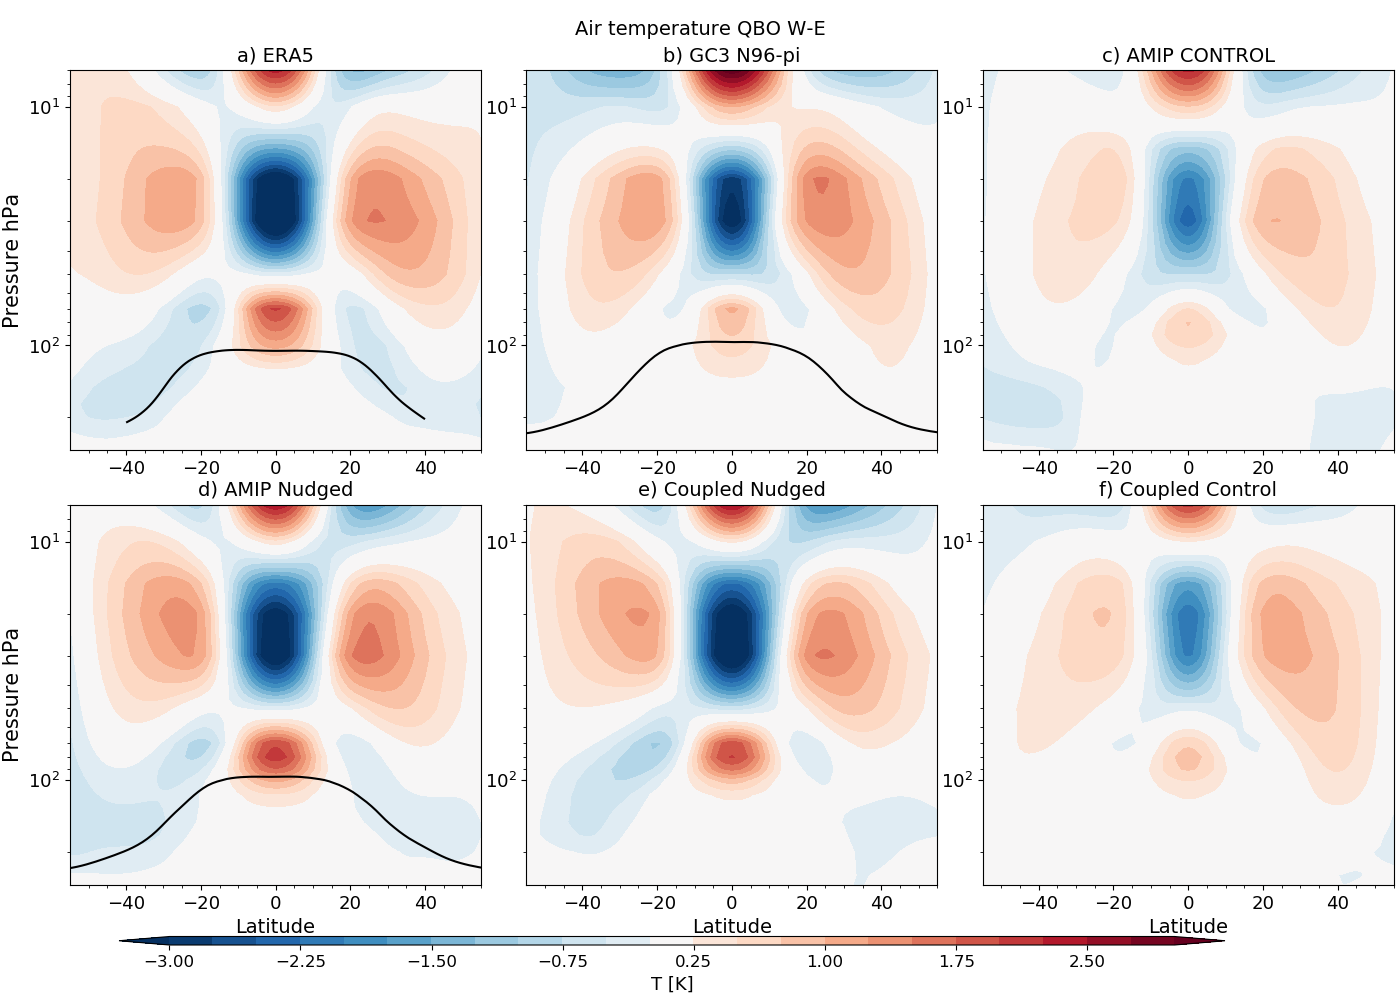
\includegraphics[width=\linewidth]{figures/zonalplotair_temperature.png}
%\caption[Zonal mean air temperature QBO difference]{As in Figure \ref{fig:zonal_u} but for air temperature.  }
%\label{fig:zonal_T}
%\end{figure} 
% 
%The nudging technique improves the zonal wind signal notably by replicating the result observed in ERA5, as expected since the nudging data is ERA5.  In the nudged runs, the wind signal near the tropopause extends poleward more than in the free-running control simulations and the peak positive anomaly found at around 70 hPa. The variability in the mid-stratosphere winds is also improved as the signal is wider reaching the subtropics. This means that the representation of shear, which modulates temperature as well, is improved with the nudging in the 20$^\circ$S-20$^\circ$N.
%
%
%
%The temperature is able to respond to the nudging within the model freely, Figure \ref{fig:zonal_T} reveals that nudging the zonal wind can also improve the air temperature variability in the lower stratosphere driven by the QBO shear. The positive temperature anomaly in the equatorial region around the 100 hPa at the tropopause level is much weaker in the GC3 N96-pi, AMIP Control and Coupled Control compared to the two nudged experiments and to ERA5. The Nudged experiments not only improve the temperature signal in the equatorial lower stratosphere but seem to overestimate this signal around the 70 hPa level. Furthermore, observations show a horse-shoe temperature anomaly pattern in the subtropics characterised by a negative anomaly that extends from 20-40 degrees north and south, a signal that is missing in the GC3 N96-pi, AMIP Control and Coupled Control experiments but is recovered in the Nudged experiments. This means that without nudging further away than 20 degrees north or south, the subtropical signal is obtained by improving the residual circulation associated with the QBO. 
%
%\begin{figure}[t!]
%\centering
% \noindent
% 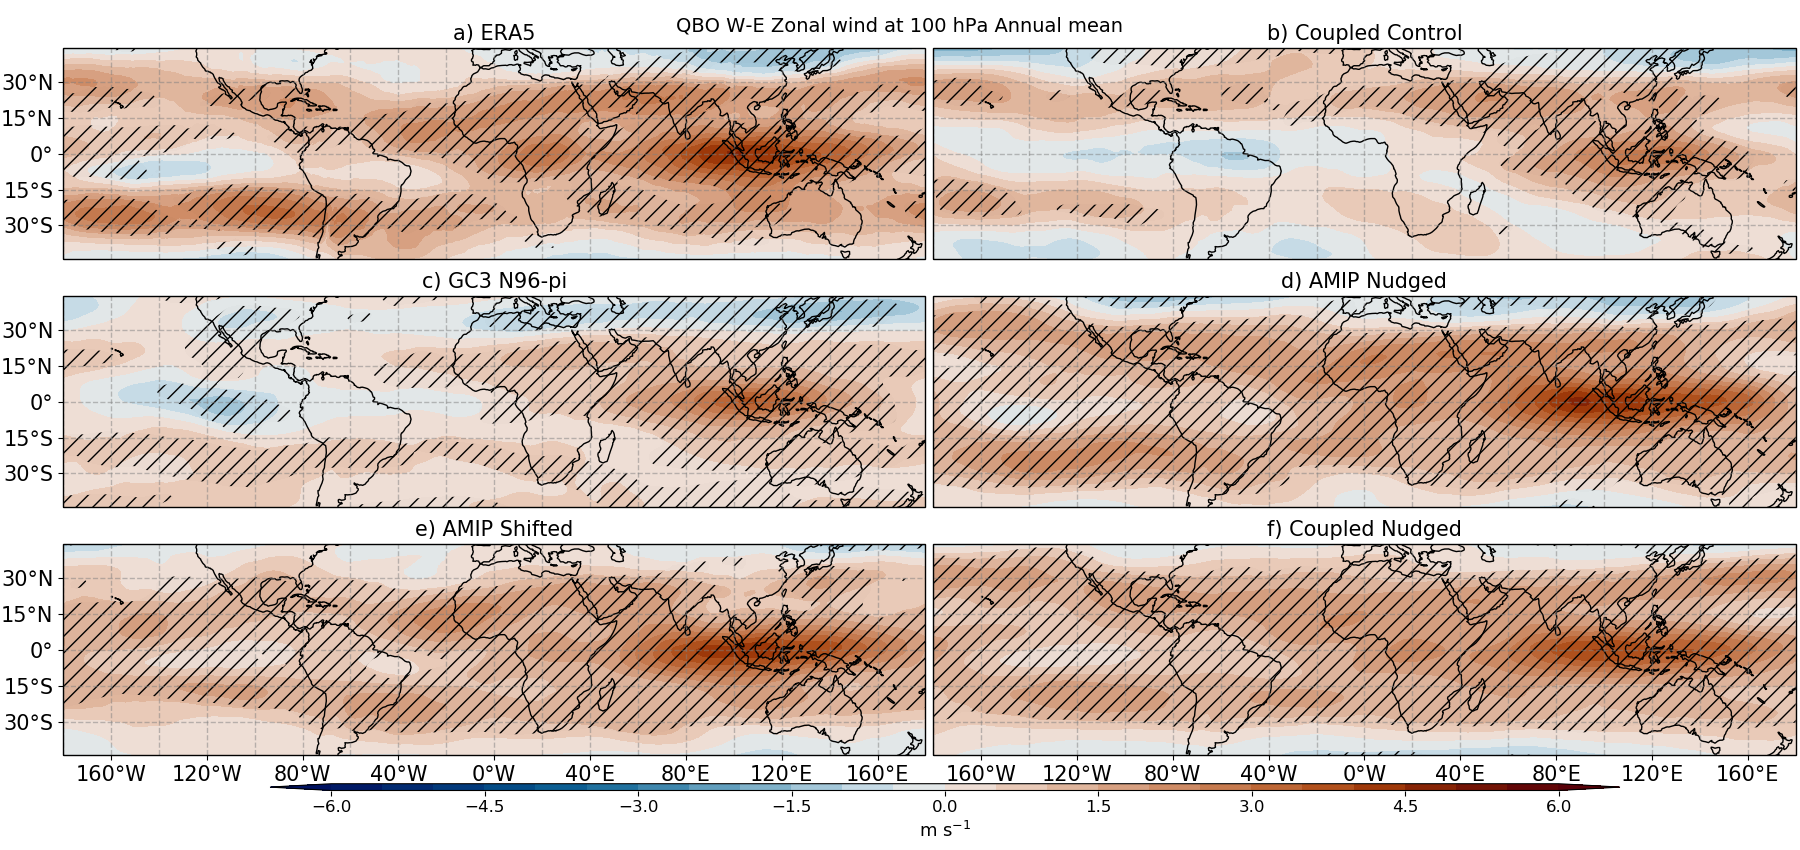
\includegraphics[width=\linewidth]{figures/ua100climqbowf.png}
%\caption[Zonal wind QBO W-E difference 100 hPa level]{Zonal wind difference in QBO W-E at the 100 hPa level. Hatching denotes significance to the 95\% level according to a Student's t-test.}
%\label{fig:ua100qbo}
%\end{figure}
%
%The spatial distribution of the wind and temperature variability associated with the QBO near the tropopause level (100-hPa level) is shown in Figures \ref{fig:ua100qbo} and \ref{fig:ta100qbo} for ERA5, GC3 N96-pi and control and nudged experiments. 
%These Figures show, first, that the free running model (seen in GC3 N96-pi and Coupled Control) is able to reproduce the zonal asymmetries in the QBO signal \citep{tegtmeier2020b} at the 100 hPa level albeit much weaker than the observed signal. The wind differences, for instance, is stronger in the Maritime continent in observations whereas the temperature signal is stronger in the Maritime continent equatorial Africa, both features reproduced sensibly by the model without nudging. 
%
%The nudging increases the magnitude of these signals at the 100 hPa level, both for the zonal wind and the temperature differences. Specifically, the temperature signal in the Nudged experiments is improved in AMIP Nudged and AMIP Shifted experiments, indicating that these differences are not associated with the underlying SST field, rather with the QBO vertical wind shear, which has been improved by nudging. 
%Results found in this analysis also indicate that the tropopause height and temperature exhibits more variability associated with the QBO than in the free-running model (not shown). 
%
%
%\begin{figure}[t!]
%\centering
% \noindent
% 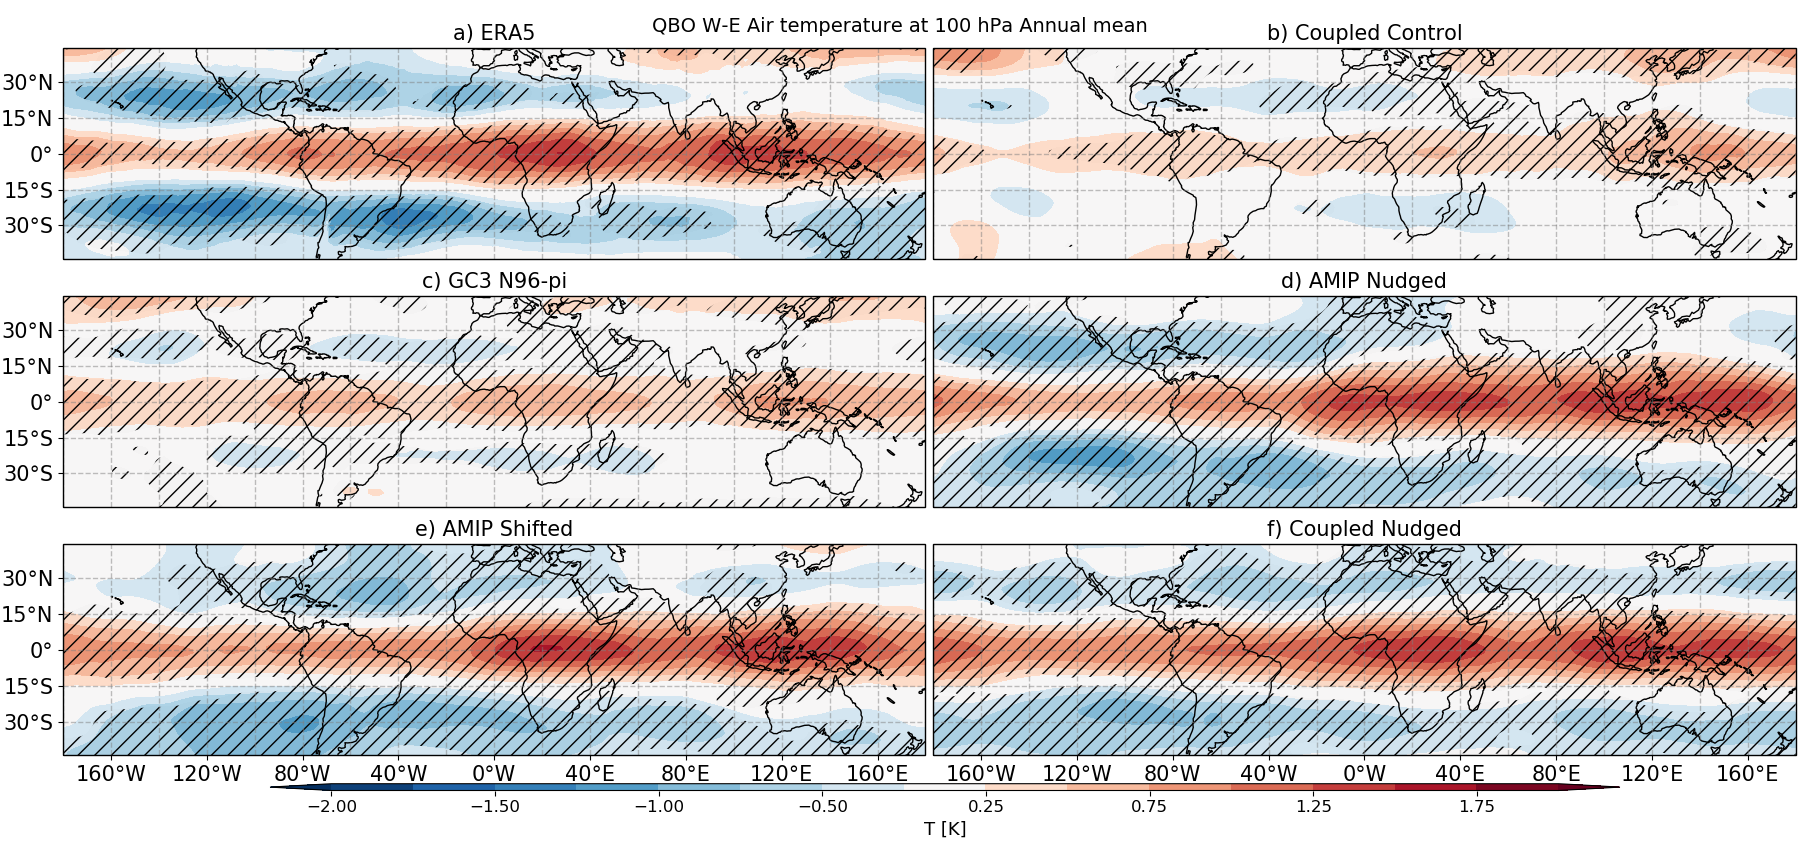
\includegraphics[width=\linewidth]{figures/ta100climqbowf.png}
%\caption[Zonal wind QBO W-E difference 100 hPa level]{As in Figure \ref{fig:ua100qbo}, but for air temperature. }
%\label{fig:ta100qbo}
%\end{figure}
%
%This section shows that the UTLS temperature and zonal wind variability are more realistic in the nudged experiments, and that this variability is not related to the underlying SSTs but rather a result of the relaxation in the equatorial stratosphere. These results indicate that these experiments are suited to investigate tropical teleconnections associated with the QBO. The hypothesis to test is that the processes that link the QBO to tropical convection should be more realistically represented in the nudged experiments than in the control experiments. %The following section investigates whether in fact surface impacts in the tropics are stronger in the nudged experiments compared to free-running simulations. 
%
%
%
%\subsection{Atmosphere-only experiments}
%
%This section describes the results of the atmosphere-only experiments: AMIP Nudged, AMIP Control and AMIP Shifted. These simulations use the CMIP6 SST dataset used for AMIP experiments, so that, in other words, the SSTs in these runs follow the observed seasonal and interannual variability of SSTs. 
%The effect of nudging on the tropical circulation is first described to evaluate whether nudging has significantly modified the mean state of the Hadley and Walker circulations. Then, the precipitation response to the QBO is compared between Nudged and Control AMIP simulations.
%
%\subsubsection{The tropical circulation}
%
%\begin{figure}[t!]
%\centering
% \noindent
% 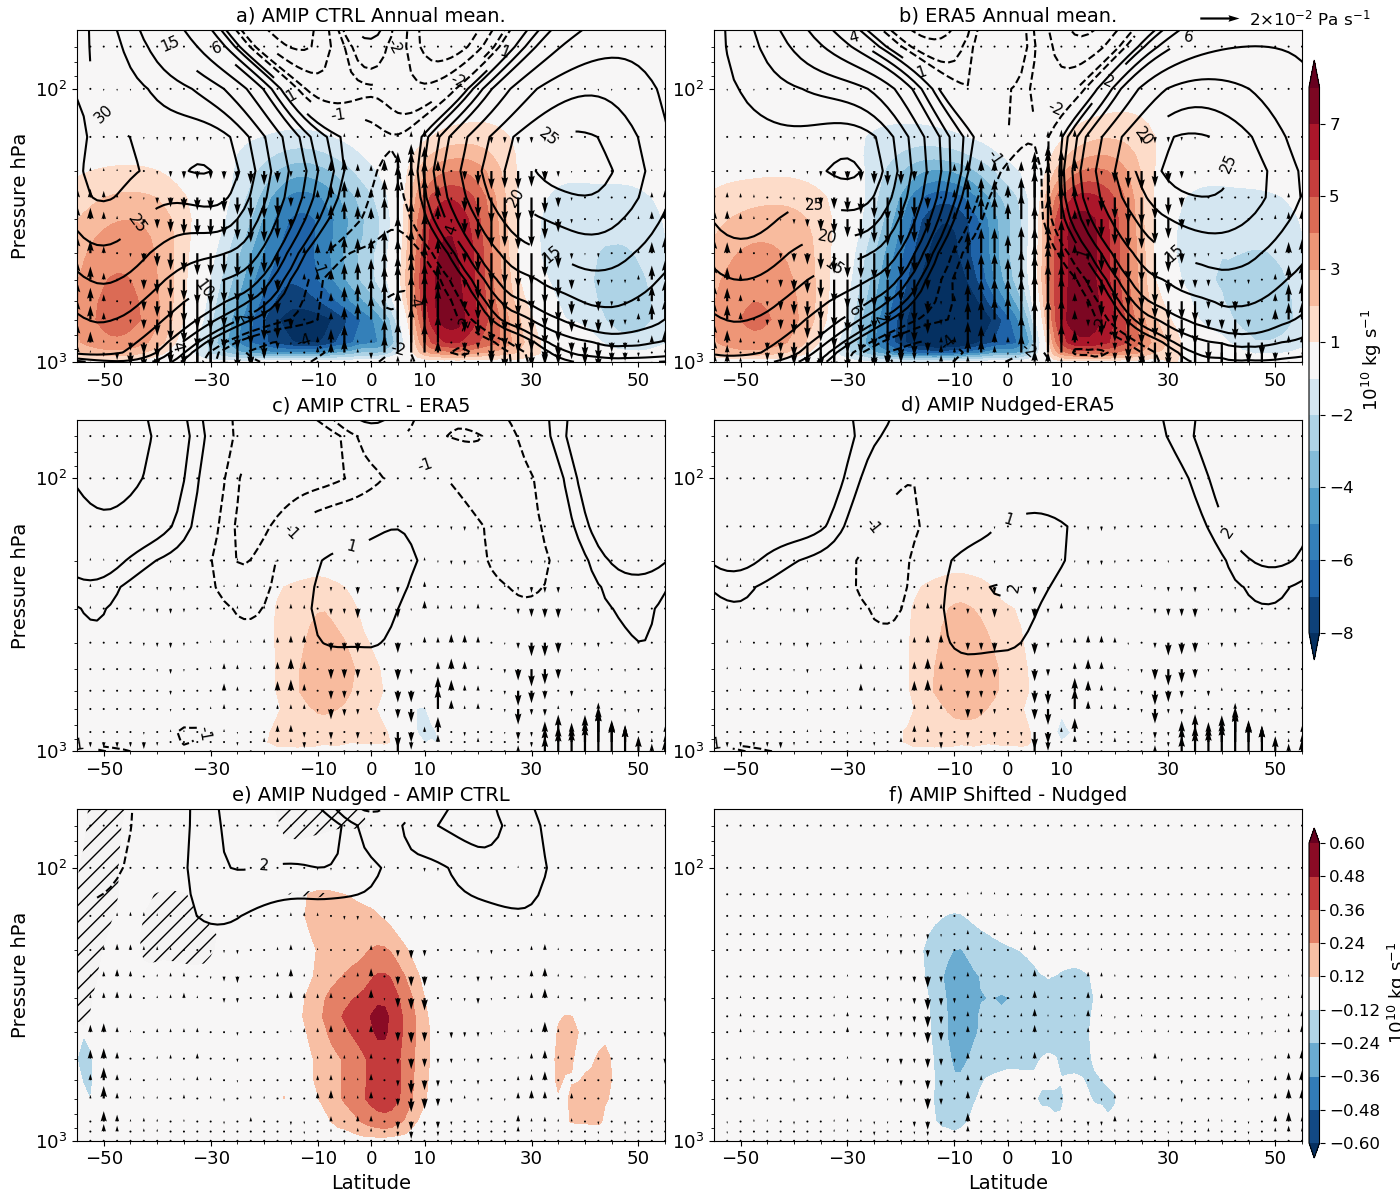
\includegraphics[width=\linewidth]{figures/suite_streamhadleyclim.png}
%\caption[Hadley cell in atmosphere-only experiments]{Hadley cell meridional mass streamfunction (shading), zonal mean zonal wind (contours) and vertical velocity (vectors). (a) Climatological mean in the AMIP Control experiment, (b) Bias in the Control experiment with respect to ERA5, differences between (c) AMIP Nudged-Control and (d) AMIP Shifted-Nudged. Note that the colorbar and scale of the vectors changes from the top to the bottom row. In (c-d), significant differences (95\% confidence level according to a Mann-Whitney two-sided test) in the streamfunction are highlighted with hatching . }
%\label{fig:hadleyamip}
%\end{figure}
%
%The mean state of the Hadley cell in the atmosphere-only configuration is weaker than in ERA5 in the 20$^\circ$S-0 region (the southern hemisphere branch in Figure \ref{fig:hadleyamip}) whereas biases in the upper-level tropical and subtropical troposphere, the model shows an easterly bias. 
%The AMIP Nudged simulation shows an improvement of this bias in the tropical and subtropical stratosphere showing positive zonal wind differences with the Control experiment in the UTLS region, i.e, correcting the easterly biases of the Control experiment. However, no significant differences in the streamfunction over the tropical troposphere are observed. Similarly, no significant differences were found in the mean-state of the Hadley circulation between the Nudged and Shifted experiments, suggesting that the variability of the nudging data is of secondary importance relative to the mean state of the nudging data. 
%
%\begin{figure}[t!]
%\centering
% \noindent
% 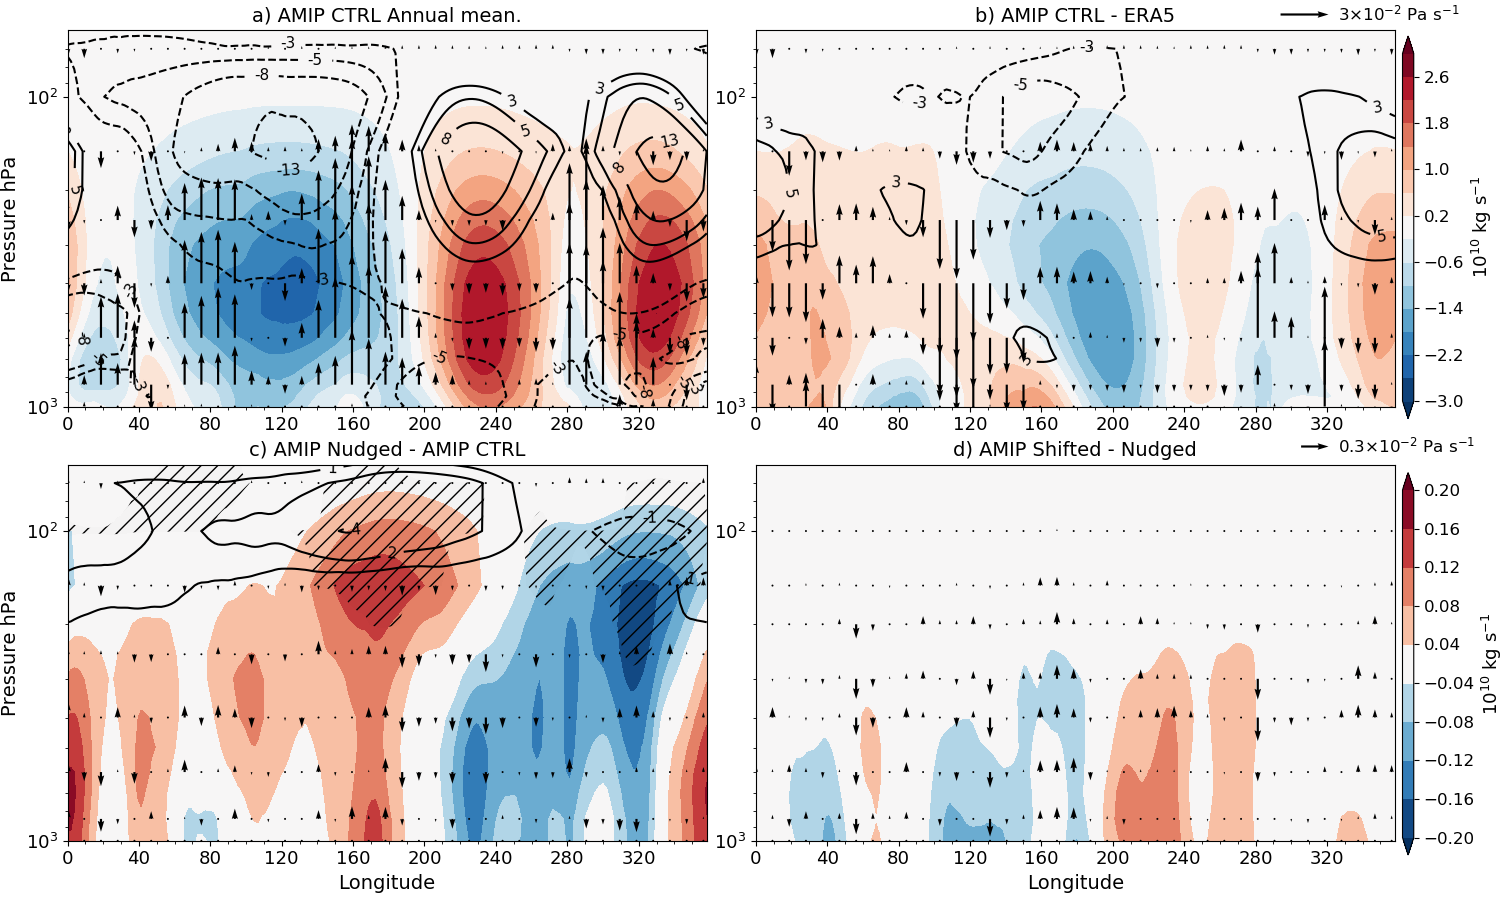
\includegraphics[width=\linewidth]{figures/suite_streamwalkerclim.png}
%\caption[Walker in atmosphere-only experiments]{Zonal mass streamfunction ($\psi$ in shading), zonal mean zonal wind (contours) and vertical velocity (vectors) averaged over the 10$^\circ$S-10$^\circ$N, as in Figure \ref{fig:hadleyamip}. }
%\label{fig:walkeramip}
%\end{figure}
%
%In turn, the Walker circulation biases in the upper troposphere are notably improved in the Nudged experiment (Figure \ref{fig:walkeramip}). The mean state of the Walker circulation is weaker in the AMIP Control simulation compared to ERA5, characterised by a weaker circulation in the Western Pacific and an easterly bias at upper levels. These two tropospheric biases in the Control experiment are reduced in the Nudged experiments, even though the relaxation is only applied above 90 hPa significant differences in the zonal wind and zonal streamfunction are observed at 200 hP near the dateline, over South America and over the Atlantic Ocean. 
%However, no significant differences are observed between the AMIP Shifted and Nudged experiments. 
%
%\begin{figure}[t!]
%\centering
% \noindent
% 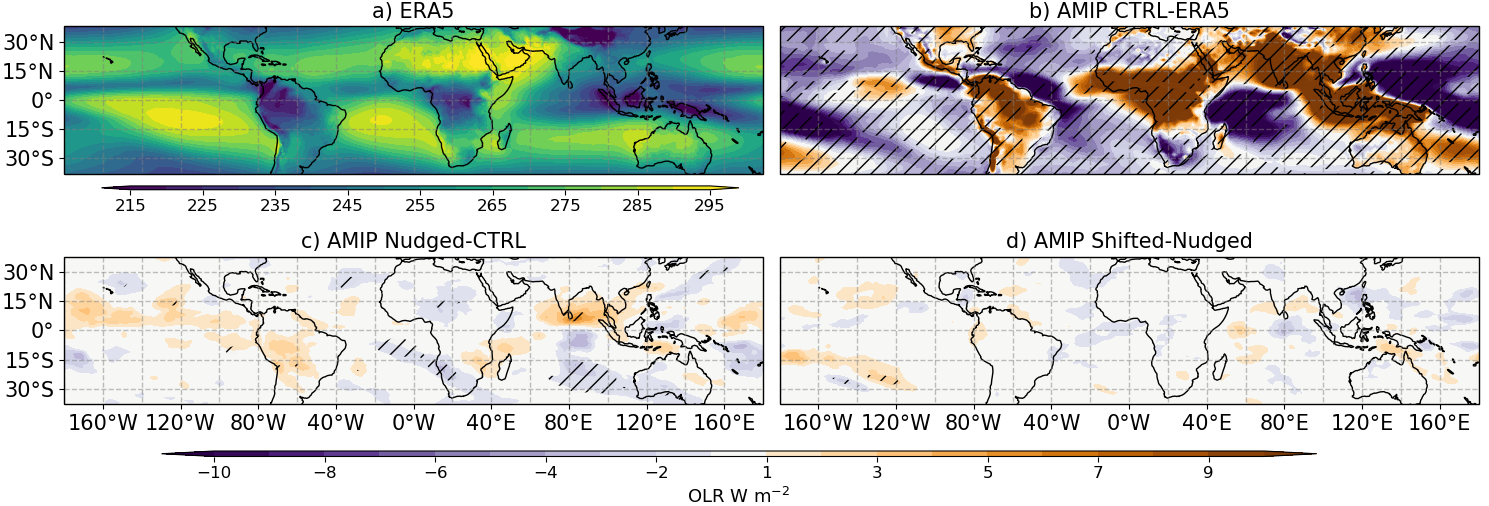
\includegraphics[width=\linewidth]{figures/olr_check.png}
%\caption[Annual mean OLR  in atmosphere-only experiments]{(a) Climatological mean OLR [W m$^{-2}$] in ERA5, (b) climatological biases in the AMIP Control simulation. (c) Differences between AMIP Nudged and Control and (d) between AMIP Shifted and Nudged. Significant (95\% confidence level) differences according to a Mann-Whitney U test in (c, d) are highlighted with hatching. }
%\label{fig:olr-mean}
%\end{figure}
%
%The mean state of the Hadley and Walker circulation at upper levels is modified in the simulations when nudging is applied, reducing the biases in the circulation within the model. However, these differences, or reductions of the biases, are smaller than the magnitude of the biases themselves, so it is unclear whether these differences are  large enough to improve other aspects of tropical climate. 
%
%\begin{figure}[t!]
%\centering
% \noindent
% 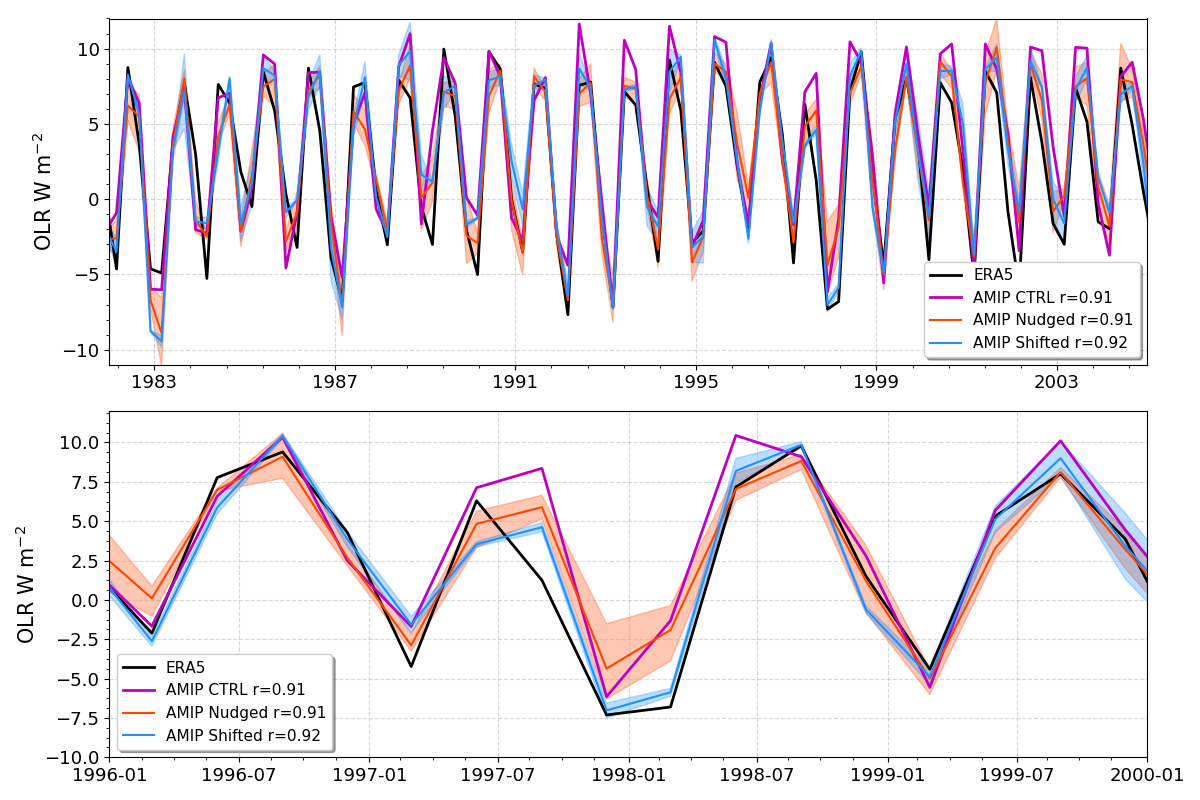
\includegraphics[width=\linewidth]{figures/olr_tseries.png}
%\caption[Tropical mean OLR time series.]{Time-series of zonal-mean equatorial [5$^\circ$S-5$^\circ$N]  OLR in ERA5 and the three amip experiments for (a) 20 yrs and a (b) 5-yr period around the 1997-1998 ENSO event. For each AMIP experiment the Pearson correlation coefficient between the experiment time-series and ERA5 is shown in the legend. }
%\label{fig:olramip_tseries}
%\end{figure}
%
%For example, Figure \ref{fig:olr-mean} shows the biases in the climatology of OLR, and the impact of Nudging on these biases. Most regions in the tropics exhibit significant and relatively large biases in AMIP Control compared to ERA5, most of which remain unchanged in the AMIP Nudged and Shifted experiments. The small and not significant differences between the two types of nudged experiments suggest a small effect of the relaxation of the zonal winds over the mean state of OLR. 
%
%Similarly, Figure \ref{fig:olramip_tseries} shows that the zonal-mean OLR time-series averaged over the deep tropics is undistinguishable between the three AMIP experiments, and the time-series of all the experiments have the same correlation coefficient with ERA5. In other words, the tropical mean OLR remains unchanged in the nudged experiments, regardles of whether the relaxation was implemented to match the SST field or whether the nudging data was shifted from the SST time-series. 
%Based on these results alone, it would appear that nudging has made little impact over the interannual variability of the tropical mean OLR. The question of whether the specific variability of OLR and precipitation associated with the QBO is also the same is now investigated in the next section. 
%
%
%\subsubsection{Precipitation response to the QBO}
%
%\begin{figure}[t!]
%\centering
% \noindent
% 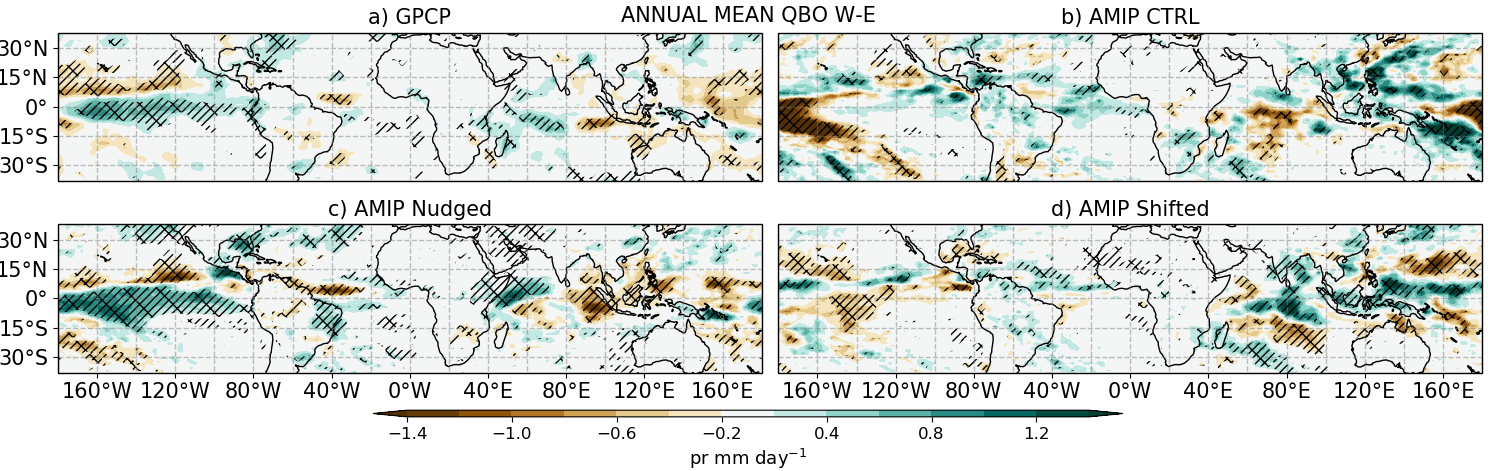
\includegraphics[width=\linewidth]{figures/pr_amip_climqbowqboe.png}
%\caption[Annual mean precipitation response in atmosphere-only experiments]{Annual-mean precipitation response (QBO W-E) in (a) GPCP, and atmosphere-only experiments: (b) AMIP CTRL, (c) AMIP Nudged and (d) AMIP Shifted.  }
%\label{fig:amip_clim}
%\end{figure}
%
%
%The annual-mean difference of precipitation between QBOWand E phases (Fig. \ref{fig:amip_clim}) in the ensemble-mean AMIP Nudged experiment matches closely the results of GPCP, characterised by an El Niño pattern in the Pacific Ocean, a weaker Atlantic ITCZ and a gradient of precipitation in the Indian Ocean during QBOW compared to QBOE. 
%In contrast, the free-running AMIP Control and the simulations with an out-of-phase relaxation of the winds with respect to the SST driving data (AMIP Shifted) show very different responses to the AMIP Nudged experiment and observations. 
%
%\begin{figure}[t!]
%\centering
% \noindent
% 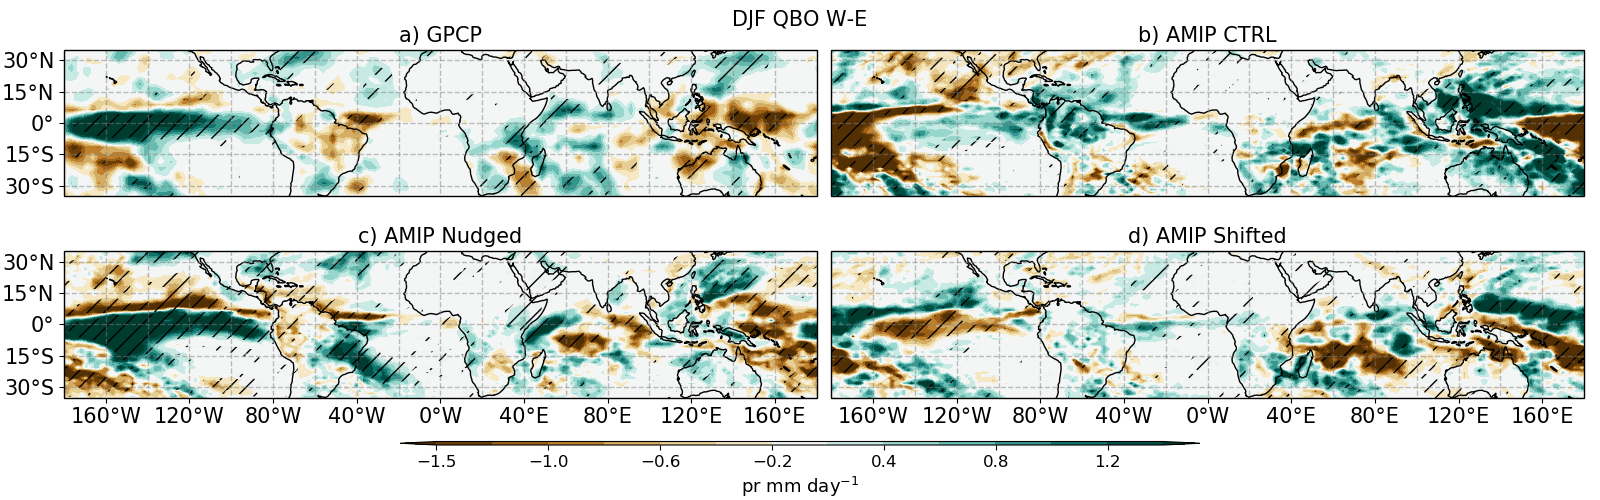
\includegraphics[width=\linewidth]{figures/pr_amip_djfqbowqboe.png}
%\caption[DJF mean precipitation response in atmosphere-only experiments]{As in Fig. \ref{fig:amip_clim} but for the DJF season. }
%\label{fig:amip_djf}
%\end{figure}
%
%A similar result is found when the composite differences only include DJF (Fig. \ref{fig:amip_djf}), so that the precipitation response in the simulations where the QBO index and the SSTs match exactly as in observations (AMIP Nudged) produce a very similar response to GPCP, whereas simulations where the QBO winds do not match the same SSTs result in different responses. 
%Results using OLR are very similar, for example, Figure \ref{fig:amip_son_olr} shows that a strong response is diagnosed in GPCP in the Indian Ocean which is reasonably reproduced in AMIP Nudged but AMIP CTRL and AMIP Shifted exhibit a very different response in the Indian Ocean and elswhere.
%
%
%
%These results suggest that the QBO winds are secondary to the effect of the SSTs for the precipitation response in these atmosphere-only experiments. The AMIP Shifted experiment has a better representation of the stratospheric variability in temperature and vertical wind shear, however, the response is entirely different to the AMIP Nudged experiments, the difference between these two experiments being the underlying SSTs. These results suggest that improving the representation of the QBO is not enough to replicate the observed response because the SST forcing dominates. 
%
%\begin{figure}[t!]
%\centering
% \noindent
% 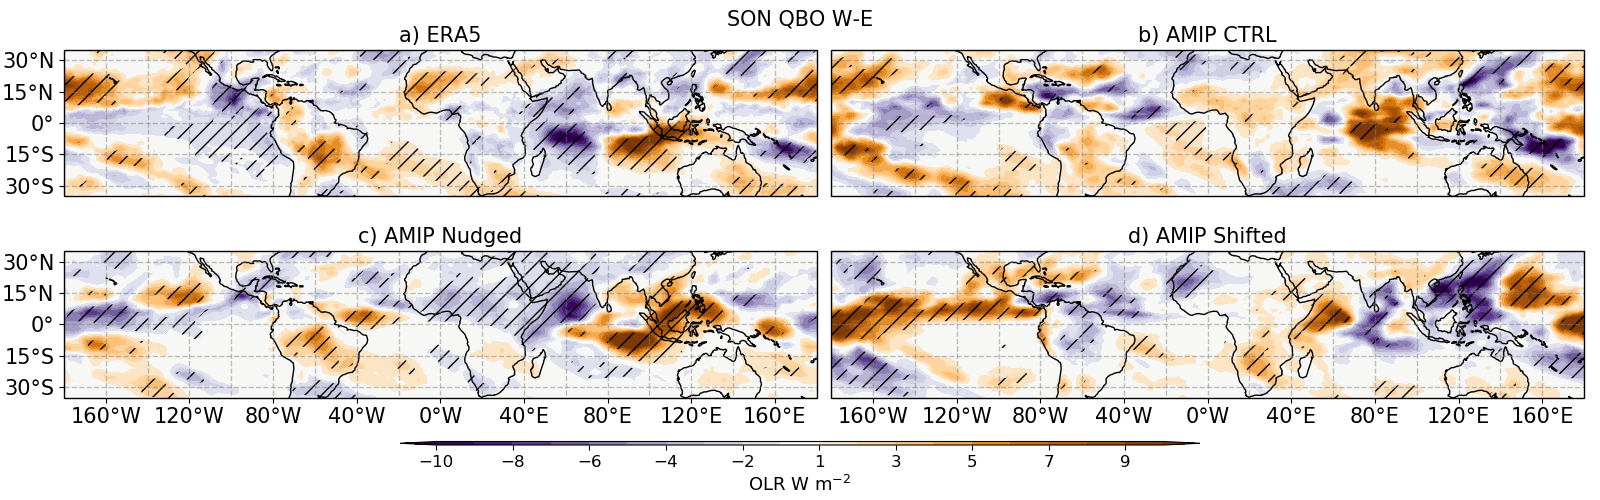
\includegraphics[width=\linewidth]{figures/olr_amip_sonqbowqboe.png}
%\caption[SON OLR response in atmosphere-only experiments]{As in Fig. \ref{fig:amip_clim} but for OLR in the SON season. }
%\label{fig:amip_son_olr}
%\end{figure}
%
%This section shows, first, that relaxing the zonal wind in the stratosphere in atmosphere-only experiments does not modify the mean state of the tropical circulation. Second, that the surface response of precipitation associated with the QBO in observations is largely associated with the underlying SSTs. The tropical mean OLR and precipitation mean state appear to be undistinguishable between Control, Nudged and Shifted experiments, whereas the composite differences between the two phases of the QBO reveal that the observed precipitation response is associated mostly with the SST anomaly pattern. However, whether the QBO has any effect over the SSTs cannot be answered in this atmosphere-only experiments, which leads to the the next section which analyses the coupled nudged experiments. 
%
%\subsection{Coupled experiments}
%
%
%This section presents the results of the coupled ocean-atmosphere experiments with (Nudged) and without (Control) relaxing the zonal wind in the tropical stratosphere. Note that all the individual experiments in this section are the same length (35 yr) and the Coupled Nudged ensemble-mean refers to the mean results of the six ensemble members with nudging.
%These coupled experiments differ only slightly from the setup used in the CMIP6 piControl experiments, analysed in section \ref{sq:cmip6_qbo}, with the atmospheric resolution of the nudged experiments matching the resolution of GC3 N96-pi and the oceanic resolution of these resolutions being the same of GC3 N216-pi. The forcing is constant in both types of runs, except that in the piControl experiments, the forcing represents conditions of the year 1850 and in the nudged experiments of the year 2000. 
%Due to these similarities, we compare the long-term CMIP6 experiments with the nudging experiments in some instances.
%
%\subsubsection{SST response}
%
%\begin{figure}[t!]
%\centering
% \noindent
% 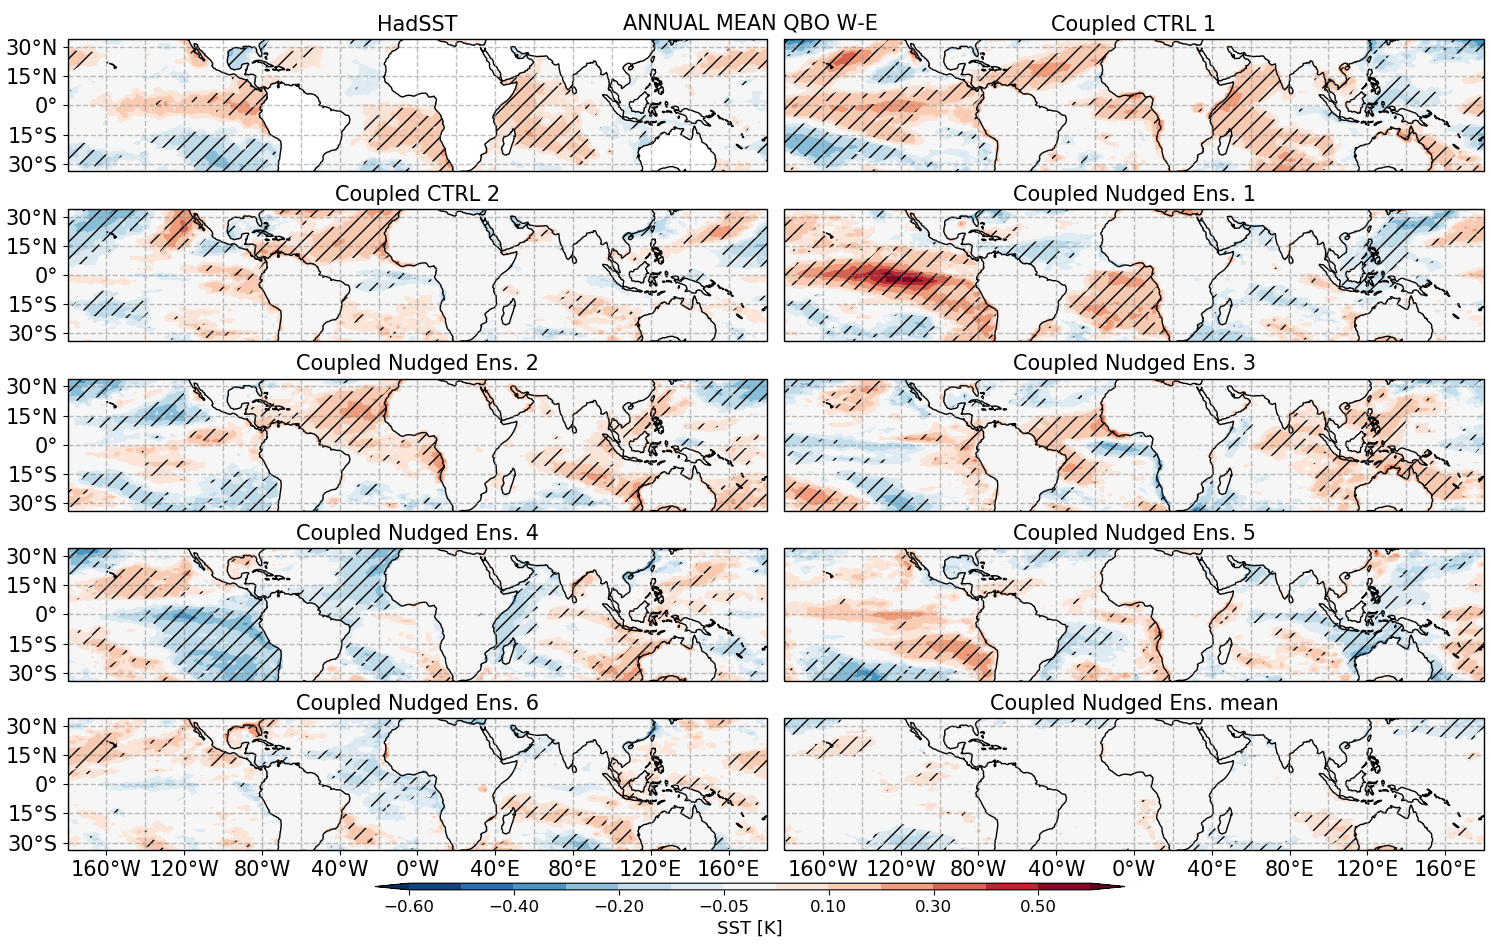
\includegraphics[width=\linewidth]{figures/sst_check_climqbowqboe.png}
%\caption[Annual mean SST response to the QBO in coupled nudged experiments]{ Annual mean SST [K] QBO W-E differences in the HadSST dataset and the Coupled Control, Coupled Nudged ensemble members and the Coupled Nudged ensemble mean. Hatching denotes significance to the 95\% confidence level according to a bootstrapping with replacement test.}
%\label{fig:sst_clim_coupled}
%\end{figure}
%
%
%The previous section shows that in atmosphere-only experiments the SST forcing dominates over any effect of the nudging, indicating that the mechanism by which the QBO influences tropical climate is involves the SSTs. In the coupled ocean-atmosphere experiments, the SSTs are able to respond and interact with any atmospheric forcing, and for that reason, this section first presents the annual mean and seasonal mean differences between the two phases of the QBO comparing coupled nudged and control experiments. 
%
%The annual mean difference in tropical SSTs between QBO phases in HadSST and each coupled experiment is shown in Figure \ref{fig:sst_clim_coupled}. In the HadSST dataset, the differences indicate a warmer East Pacific, and equatorial Atlantic and Indian Oceans. The first control experiment shows a very similar response in the Pacific and Indian Oceans whereas the results of the second control experiment only agree with the HadSST results in the subtropical North Atlantic and in the Western Pacific. 
%The nudged experiments, in turn, show a number of different responses, with differences being significant and positive in some regions in one ensemble and of another sign and unsignificant in other ensembles. 
%
%\begin{figure}[t!]
%\centering
% \noindent
% 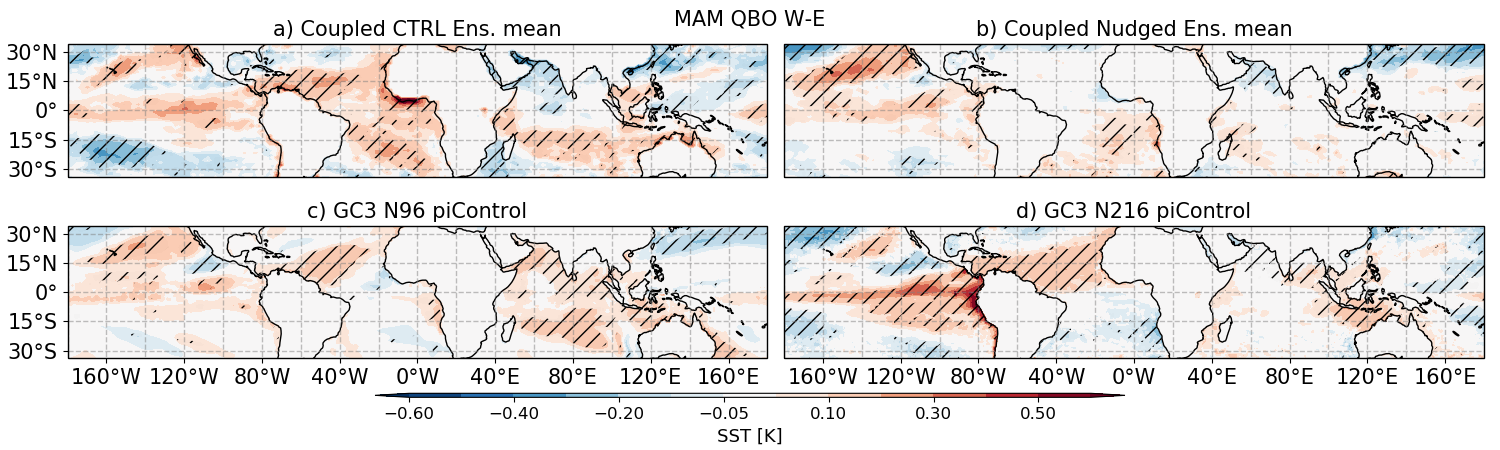
\includegraphics[width=\linewidth]{figures/sstseasonal_mamqbowqboe.png}
%\caption[SST response in MAM to the QBO in coupled nudged experiments]{ SST differences between QBO phases in MAM in (a) Coupled Control ensemble mean (2-member), (b) Nudged Coupled ensemble mean (6 members) and in the CMIP6 (c) GC3 N96-pi and (d) GC3 N216-pi.}
%\label{fig:sst_mam_coupled}
%\end{figure}
%
%The ensemble-mean response shows that averaging over all ensembles results in a weak mean response, with only some differences being different than zero and significant, for example the positive differences found over the coast of Australia and the subtropical Central Pacific. 
%In specific seasons, such as MAM (\ref{fig:sst_mam_coupled}), the SST response also appears to be stronger in the tropics in the free-running Coupled Control experiments than in the nudged experiments. 
%In MAM, a positive difference found in the Atlantic, Indian and Pacific Oceans in the CMIP6 experiments is also found in the control experiments but this response is weaker in the ensemble-mean of the nudged experiments.
%The nudged experiments show a relatively large difference in the eastern subtropical Pacific reaching the coast of California, in agreement with the control experiments.
%
%\begin{figure}[t!]
%\centering
% \noindent
% 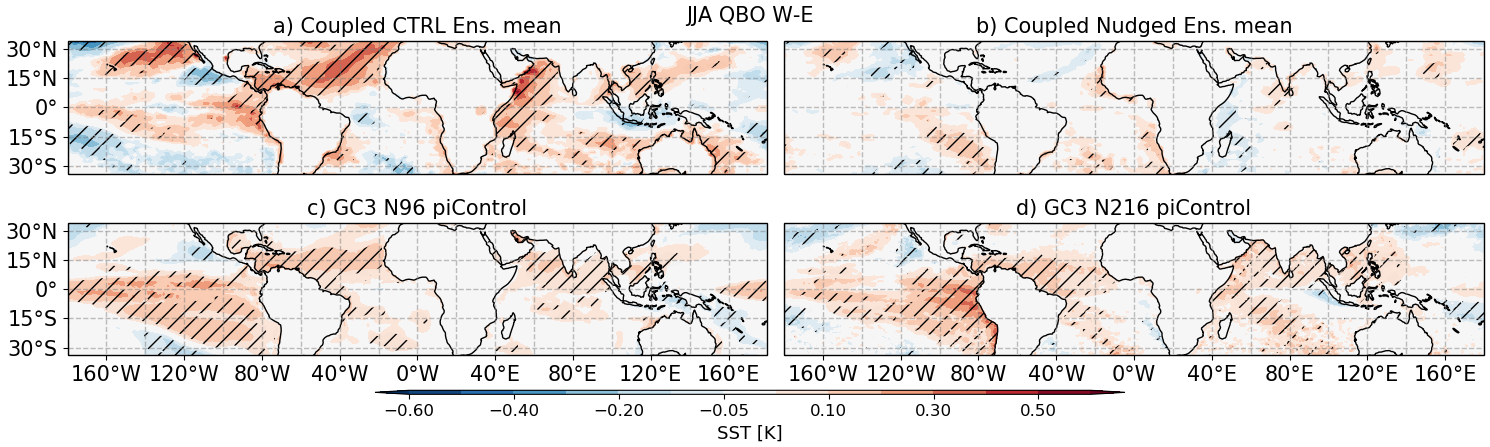
\includegraphics[width=\linewidth]{figures/sstseasonal_jjaqbowqboe.png}
%\caption[SST response in JJA to the QBO in coupled nudged experiments]{As in Fig. \ref{fig:sst_mam_coupled} but for JJA.}
%\label{fig:sst_jja_coupled}
%\end{figure}
%
%The pattern of positive anomalies in the equatorial Central and Eastern Pacific, as well as in the Atlantic Ocean, appears in the control and CMIP6 experiments in most months. 
%In boreal summer (Fig. \ref{fig:sst_jja_coupled}), the patterns are particularly strong in the Coupled Control ensemble mean in the Atlantic and Indian Oceans. However, the Nudged experiments show a very weak mean response in the tropics, only a warm difference found in the western coast of South America. 
%For the other seasons, SON and DJF, similar results are found (not shown) in which the ensemble mean of the control experiments agrees well with the CMIP6 experiments, whereas weaker responses are found in the nudged experiments.
%
%These results suggest that the SST response to the phase of the QBO in the nudged experiments is not significantly larger in the experiments compared to the control or the CMIP6 experiments, especially in equatorial regions. 
%In other words, the simulations with a stronger temperature signal associated with the QBO show the seemingly weakest response to the phase of the QBO.
%The lack of robust and large patterns of SST anomalies suggests that the precipitation response may also be weaker in the ensemble mean of experiments with nudging, which is the topic of the next section.
%
%\subsubsection{Precipitation response}
%
%\begin{figure}[t!]
%\centering
% \noindent
% 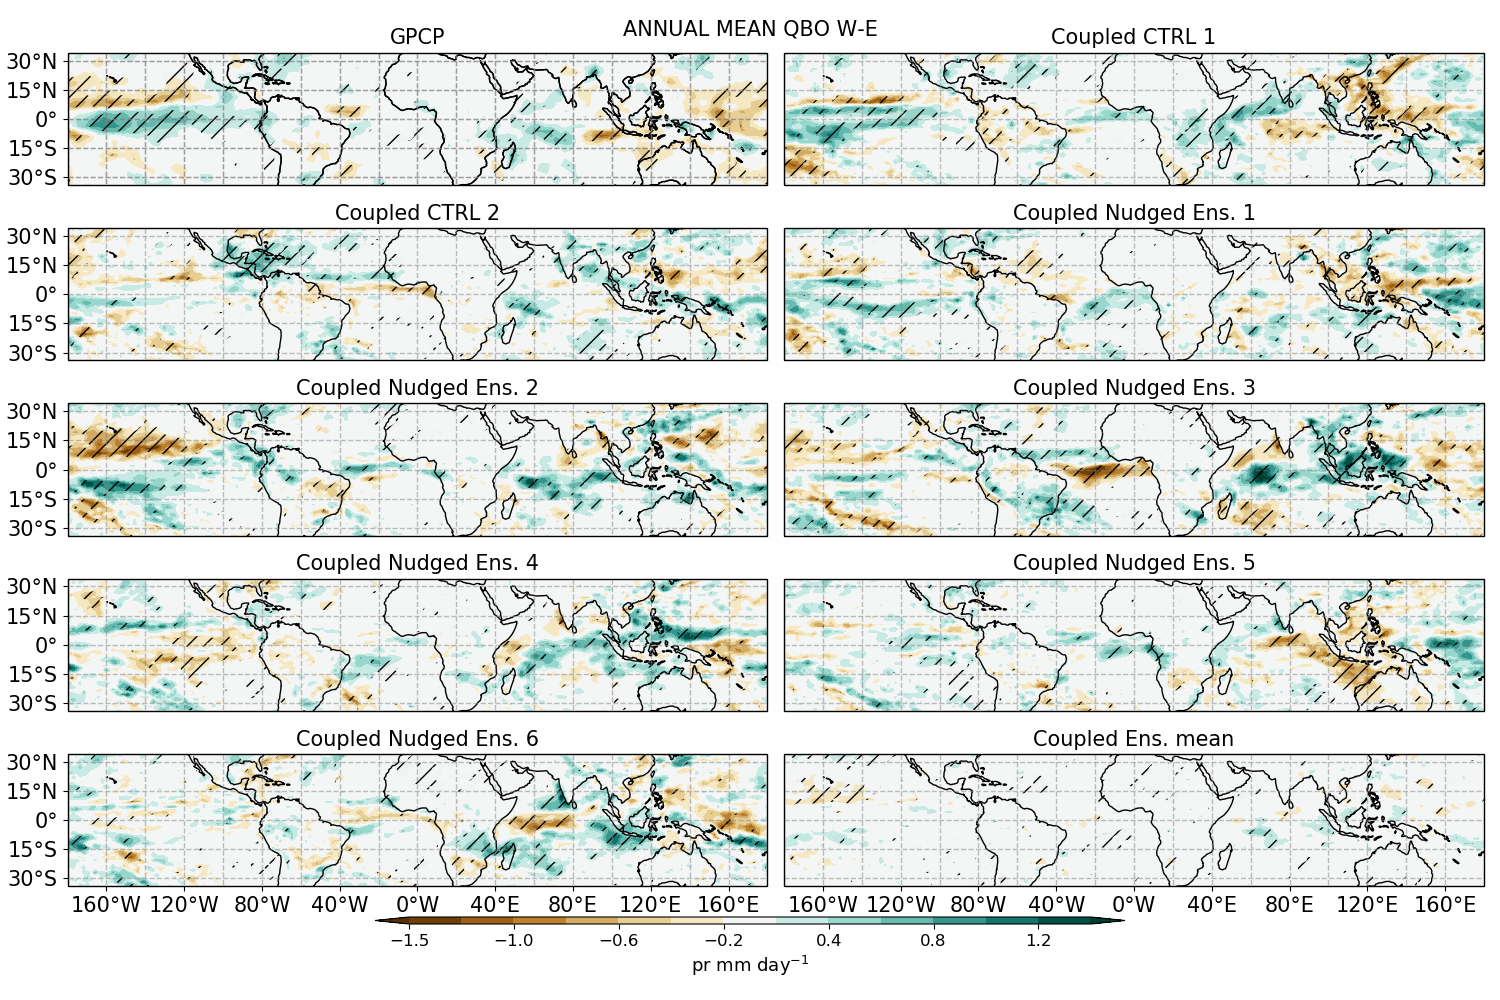
\includegraphics[width=\linewidth]{figures/pr_check_climqbowqboe.png}
%\caption[Precipitation response to the QBO in coupled nudged experiments]{ Annual mean precipitation QBO W-E differences in GPCP, Coupled Control, Coupled Nudged ensemble members and the Coupled Nudged ensemble mean. Hatching denotes significance to the 95\% confidence level according to a bootstrapping with replacement test.}
%\label{fig:pr_clim_coupled}
%\end{figure}
%
%
%The annual mean difference between QBO phases (Fig. \ref{fig:pr_clim_coupled}) in each coupled experiment reveals a strong variability of the precipitation response, suggesting an important role of long-term variability for these responses. 
%In particular, the control experiments show two significant responses: the first control experiment shows a significant El Niño-like response over the Central and Eastern Pacific Ocean, whereas the second control experiment shows a northward shift of the Atlantic ITCZ and a wetter Caribbean Sea.
%Precipitation differences in the Indian Ocean and continent are also significant in both of these two coupled experiments, even though the pattern and magnitude of the difference is not a close match, both simulations suggest a wetter western Indian Ocean and continent. 
%Note that these three responses found in the Coupled Control experiments in this setup were also observed over the longer GC3 N96 and N216-pi experiments, described previously in this chapter.
%
%
%
%The nudged experiments show various different responses (Fig. \ref{fig:pr_clim_coupled}), with several regions showing significant responses of one sign in one ensemble member and another, also significant, response of an opposite sign in a different ensemble just as in the SST differences of Figure \ref{fig:sst_clim_coupled}. In most ensemble members, the stronger responses are seen over the ocean rather than over land.
%The nudged ensemble mean shows regions with a significant response but the difference value in signficant regions is too small to be represented by the colorbar, indicating a weak response. 
%
%\begin{figure}[t!]
%\centering
% \noindent
% 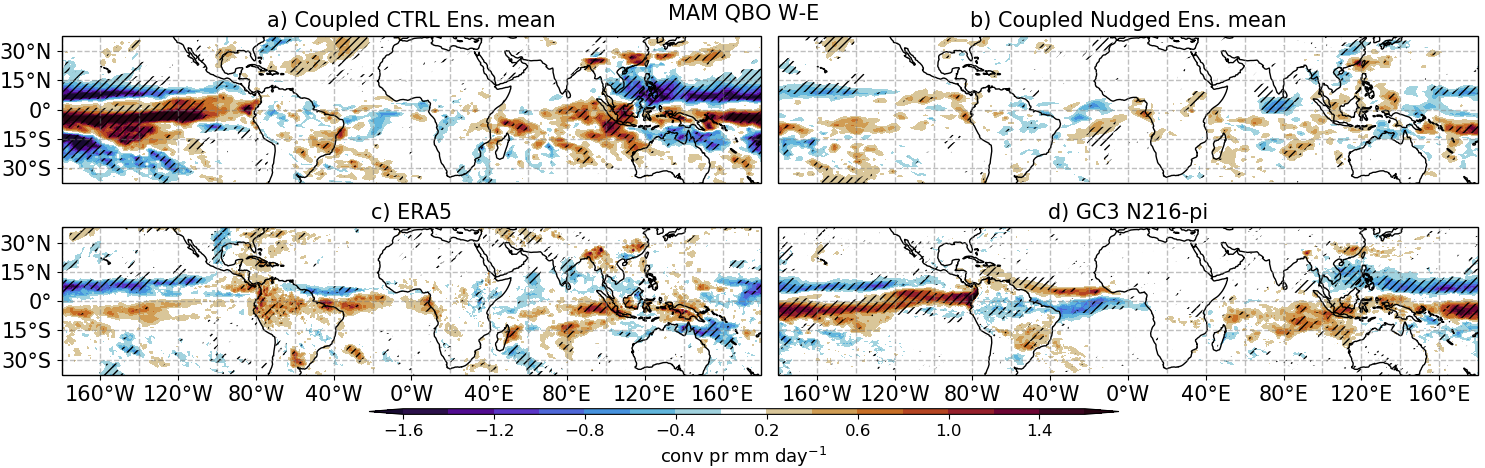
\includegraphics[width=\linewidth]{figures/conv_prseasonal_mamqbowqboe.png}
%\caption[ Convective precipitation response in MAM]{As in Fig. \ref{fig:sst_mam_coupled} but for convective precipitation.}
%\label{fig:conv_pr_mam_coupled}
%\end{figure}
%
%
%
%The differences in a specific season are also relatively weak in the ensemble mean of the nudged experiments. 
%For instance, in boreal spring, the differences in convective precipitation (Figure \ref{fig:conv_pr_mam_coupled}) show a wetter equatorial Pacific and a drier band at 10$^\circ$N during QBOWthan E in the control ensemble mean and CMIP6 experiments, whereas the nudged experiments only show the dry response. The Coupled Control ensemble mean and CMIP6 experiments also show agree on the sign and pattern of the response in the Western Pacific and Indian Ocean, characterized by dry anomalies in the Western Pacific ITCZ, the Philippines and the South China Sea, whereas wetter anomalies are observed in the Indian Ocean. 
%In contrast, the composite mean results in the nudged experiments show unsignificant responses in these above mentioned regions. 
%
%
%
%In other seasons, the control experiments also match the results of the CMIP6 experiments, whereas the nudged experiments show a weaker or no response. For example, in boreal summer (Fig. \ref{fig:conv_pr_jja_coupled}) the CMIP6 experiments and Coupled Control experiments show a northward shift of the Atlantic ITCZ, a wetter Caribbean Sea and Indian Oceans and a drier eastern Pacific. The nudged experiments are in reasonable agreement in the Indian Ocean, indicating wetter conditions during QBOWthan E.
%Similarly, the effects over the Indian Ocean in SON found for the CMIP6 experiments in section \ref{sq:cmip6_qbo}, are also seen in the Coupled Control experiments, but not in the nudged experiments (not shown).
%
%
%\begin{figure}[t!]
%\centering
% \noindent
% 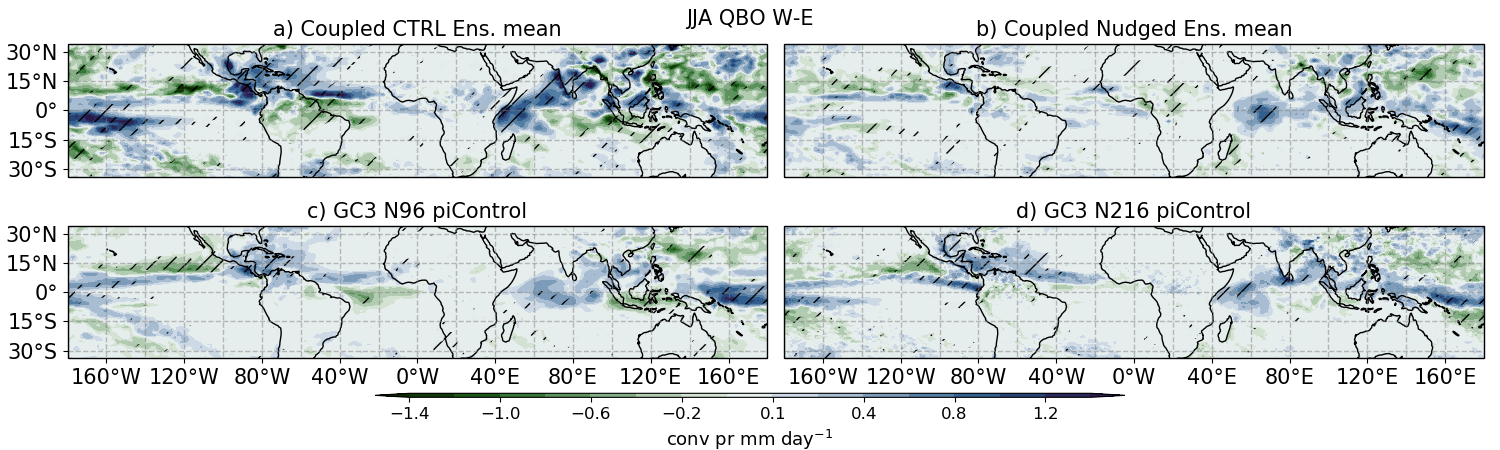
\includegraphics[width=\linewidth]{figures/conv_prseasonal_jjaqbowqboe.png}
%\caption[ Convective precipitation response in JJA]{As in Fig. \ref{fig:conv_pr_mam_coupled} but for JJA.}
%\label{fig:conv_pr_jja_coupled}
%\end{figure}
%
%The results of the precipitation response agree with the previous results that analysed the SST differences. There is no evidence that the nudged experiments result in a stronger surface response to the phase of the QBO, even though the UTLS temperature variability associated with the QBO has been increased and improved in the nudged experiments. 
%However, whether the mean state and variability of the tropical circulation has been modified could offer an explanation to these results.
%
%\subsubsection{Tropical circulation response and the IOD}
%
%\begin{figure}[t!]
%\centering
% \noindent
% 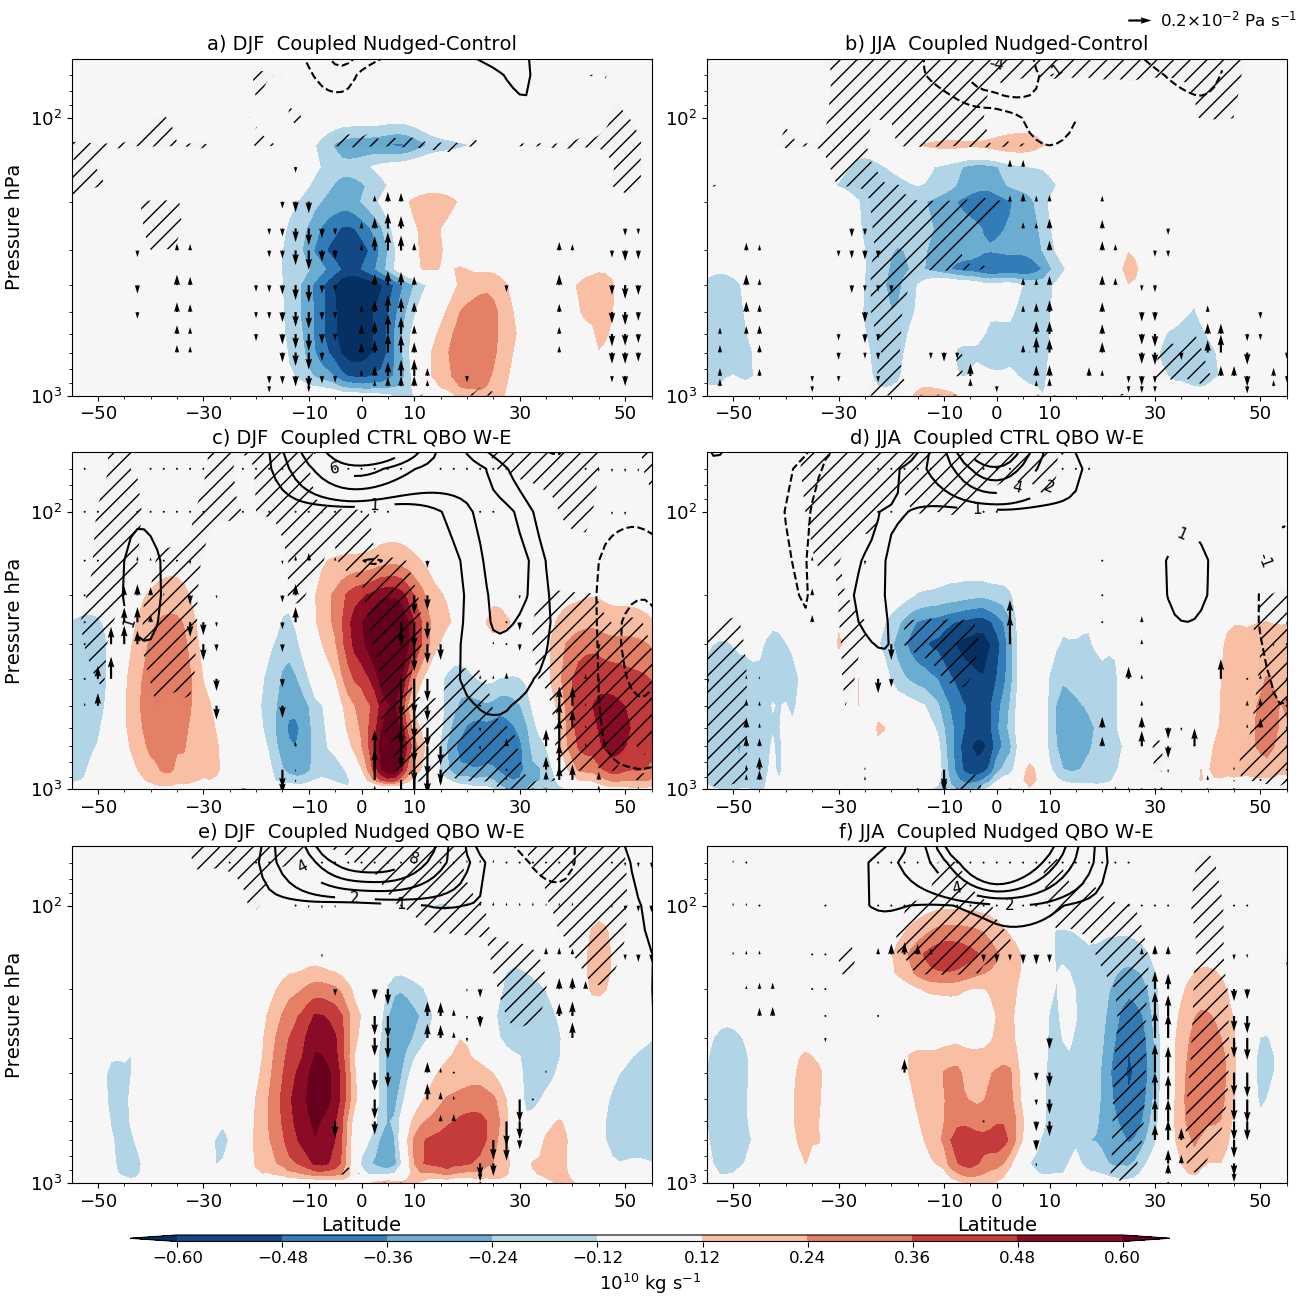
\includegraphics[width=\linewidth]{figures/suite_coupledhadley.png}
%\caption[Hadley circulation in coupled nudged experiments.]{Hadley circulation differences in meridional mass streamfunction (shading), zonal wind (contours) and vertical velocity (vectors). (a, b) show the seasonal mean differences between Nudged and Control coupled experiments in (a) DJF and (b) JJA. (c-f) show the QBO W-E differences for the (c-d) Control and (e-f) Nudged experiments for (c,e) DJF and (d,f) JJA. In all panels, hatching denotes significant differences in the streamfunction to the 95\% confidence level according to the bootstrapping method, whereas for the zonal wind and omega, only significant differences are shown.}
%\label{fig:hadley_coupled}
%\end{figure}
%
%The variability of the tropical circulation in the atmosphere-only experiments was found to be dominated by the SST forcing in the previous section. However, to the mean state of the upper-level branch of the Walker circulation was slightly different in the AMIP Nudged experiments compared to the Control. 
%To understand whether similar changes to the mean state or variability of the tropical circulation are observed in the coupled experiments, Figures \ref{fig:hadley_coupled} and \ref{fig:walker_coupled} show the impact of nudging on the mean state and variability of the Hadley and Walker circulations, respectively.
%
%The nudging appears to modify the mean state of the Hadley circulation in both DJF and JJA seasons (Figure \ref{fig:hadley_coupled}). Significant changes in the tropical UTLS streamfunction are observed in both seasons, and in DJF changes to the vertical velocity in the tropics suggest a strengthening of the Hadley cell when nudging is applied but very small changes are observed in JJA. 
%
%\begin{figure}[t!]
%\centering
% \noindent
% 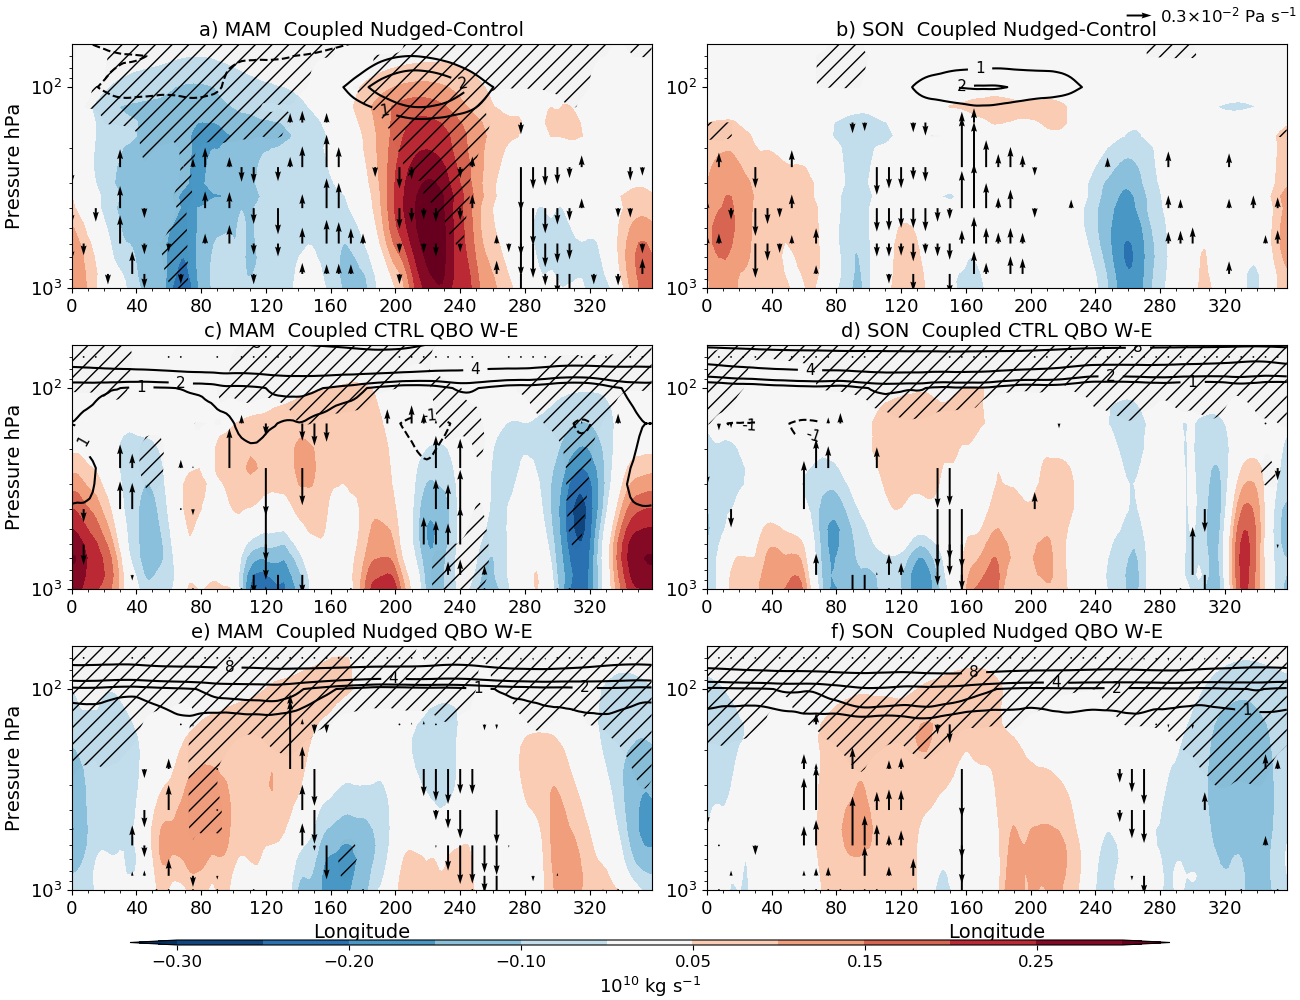
\includegraphics[width=\linewidth]{figures/suite_coupledwalker.png}
%\caption[Walker circulation in coupled nudged experiments.]{Walker circulation differences in zonal streamfunction (shading), zonal wind (contours) and vertical velocity (vectors). (a, b) show the seasonal mean differences between Nudged and Control coupled experiments in (a) MAM and (b) SON. (c-f) show the QBO W-E differences for the (c-d) Control and (e-f) Nudged experiments for (c,e) MAM and (d,f) SON. In all panels, hatching denotes significant differences in the streamfunction to the 95\% confidence level according to the bootstrapping method, whereas for the zonal wind and omega, only significant differences are shown.}
%\label{fig:walker_coupled}
%\end{figure}
%
%The difference QBO W-E in the tropospheric state of the Hadley cell in both seasons is considerably different between Nudged and Control experiments (Figs. \ref{fig:hadley_coupled}c-f). 
%In DJF, the Nudged ensemble-mean shows anomalous descent over the 10$^\circ$N latitude band and significantly higher values of the streamfunction at the equator extending into the lower troposphere. Similarly, the zonal wind in this season shows a positive anomaly extending as far down as 500 hPa at 20-30$^\circ$N, indicative of changes to the sub-tropical jet position and strength, documented previously \citep[e.g.][]{garfinkel2010}.
%
%Even though the Nudged experiments show stronger zonal wind anomalies in the equatorial stratosphere in both seasons, the response of the northern hemisphere subtropical jet is not observed, and the differences in the streamfunction and vertical velocity appear opposite to that of the Control experiments in DJF. 
%The same contrast is observed in JJA, with the Control and Nudged experiments exhibiting very different responses. Notably, the streamfunction and vertical velocity in the Nudged experiments in this season shows a dipole signal in the Northern Hemisphere with positive and negative anomalies indicating anomalous ascent at 30$^\circ$N and descent at 50$^\circ$N.
%
%The mean Walker circulation is also affected by the nudging (Fig. \ref{fig:walker_coupled}). As in the AMIP experiments, the upper-level zonal wind and streamfunction is modified by the nudging, only that in the coupled experiments, significant differences are observed in the lower troposphere over the Indian Ocean and the Eastern Pacific. 
%In the UTLS region above the Indian and Pacific Oceans, the nudging is forcing the zonal wind towards ERA5, thus reducing the biases in the model (see e.g. Figure \ref{fig:swalker}). In other words, not only biases in the variability of the zonal winds in the lower stratosphere are alleviated by the nudging but also the mean state of the upper-level branch of the Walker circulation. However, the latter may also mean that the variability of the Walker circulation is overconstrained when nudging is applied. 
%
%The response of the Walker circulation to the QBO is different in nudged versus control experiments (Fig. \ref{fig:walker_coupled}c-f). While in MAM, the control results suggest a weaker state of the Walker circulation or an El Niño-like pattern with anomalous ascent in the Eastern Pacific, the nudged simulations show the opposite. 
%In turn, in SON, while the control experiments show anomalous ascent in the western Indian Ocean, the nudged experiments show ascent over the eastern Indian Ocean. 
%
%The nudging appears to modify the mean state and variability of the tropical circulation to a certain extent. However, the differences shown in Figures \ref{fig:hadley_coupled} and \ref{fig:walker_coupled} are relatively small compared to the climatological values,  but clearly some of these differences are still significant. 
%
%Results in a previous section demonstrated that in the CMIP6 pre-industrial control experiments a statistically significant relationship is found between the IOD and ENSO, and the QBO (Fig. \ref{fig:iod_barplot}). 
%Positive events of the IOD and ENSO are more commonly found during QBOW than E, and a convective precipitation index of the IOD and the SST EN3.4 index are also positive during QBOW and negative during QBOE. 
%Figure \ref{fig:iod_suites} revisits these relationships in the coupled experiments. 
%
%\begin{figure}[t!]
%\centering
% \noindent
% 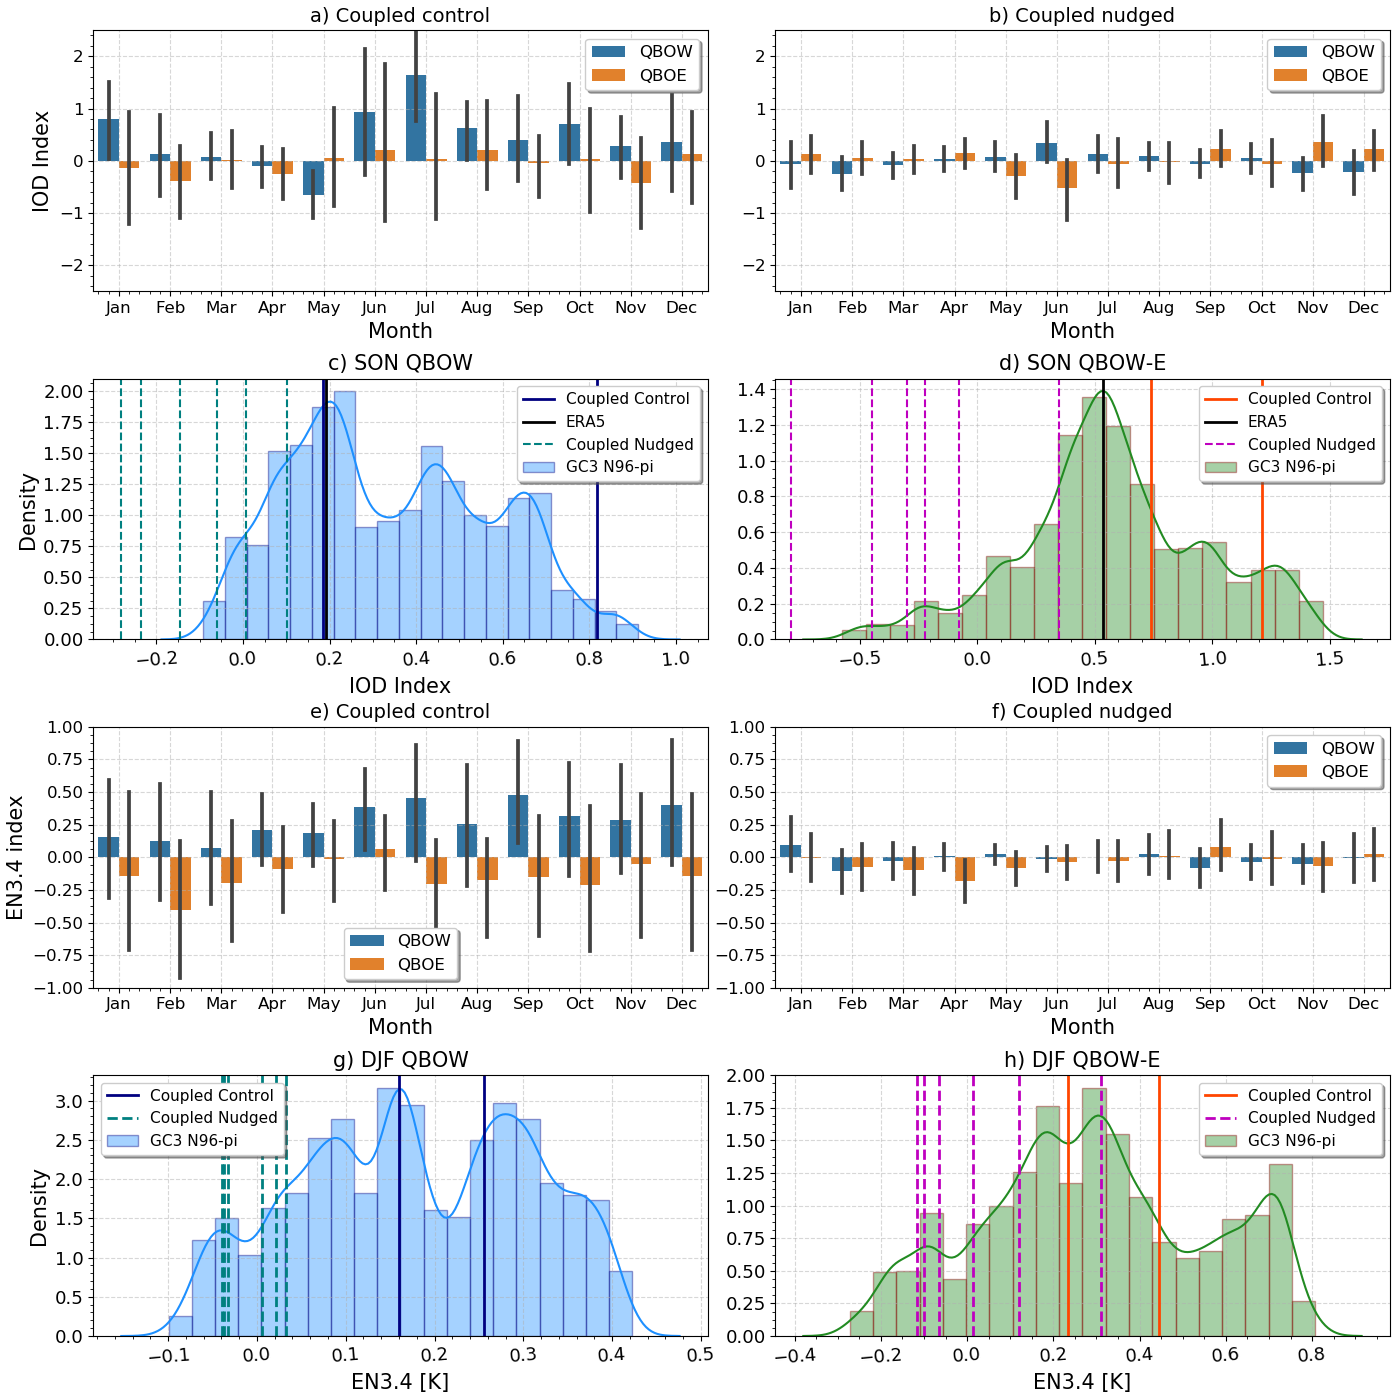
\includegraphics[width=\linewidth]{figures/iod_suites.png}
%\caption[IOD and ENSO indices in nudged versus control experiments]{(a, b) Monthly-mean IOD convective precipitation index [mm day$^{-1}$] in coupled (a) control and (b) nudged ensemble-means separated by QBO phase. (c, d) Probability density functions (PDFs) of the IOD convective precipitation index for (c) the mean SON during QBOW months and (d) the SON difference between QBO W-E. The PDF is obtained from the 500 yrs of the GC3 N96-pi by bootstrapping 10,000 times into 35-yr periods and obtaining the averages and differences in each subsample. The mean indices for the Coupled Control and Nudged experiments, as well as for ERA5 are also shown. (e, f) Monthly-mean EN3.4 index [K] in the ensemble mean (e) Coupled control and (f) Coupled Nudged simulations separated by QBO phase.   }
%\label{fig:iod_suites}
%\end{figure}
%
%The mean IOD index is positive during QBOW and negative during QBOE in the Coupled Control ensemble in boreal fall and early winter (Fig. \ref{fig:iod_suites}a), in agreement with results from the CMIP6 experiments. In contrast, the mean IOD index is close to zero in the Coupled Nudged ensemble without any clear relationship between the index and the QBO phase in any month (Fig. \ref{fig:iod_suites}b). 
%These results suggest that no consistent relationship is found across the six ensemble members where nudging was applied in the simulation. 
%However, these results may simple be due to sampling of the ocean-atmosphere state used for the nudged experiments, in other words, possibly due to decadal variability in the GC3.1 configuration.
%
%For that reason, the CMIP6 GC3 N96-pi is used to investigate whether the results of the Nudged and Control experiments are also seen in periods of similar length in that long 500 yr simulation. While this comparison is not perfect due to differences in ocean resolution and forcing, the model setup and parametrisations, and atmospheric resolution is otherwise the same between GC3 N96-pi and these experiments. 
%The simulation is repeatedly sampled at random for 35 yr continous periods, and the SON IOD index is computed each time to construct a probability distribution.  
%
%Figure \ref{fig:iod_suites}c shows that the IOD index during QBOW in GC3 N96-pi is more frequently positive, as shown in the previous section, but in some 35-yr periods a negative mean index during QBOW can be observed in this simulation. The two Coupled Control simulations and ERA5 show a positive mean IOD index during QBOW whereas four out of the six Coupled Nudged simulations show a negative index. 
%
%The previous section showed not only that positive IOD indices and events are more frequent during QBOW, but also that the opposite is true for QBOE. Figure \ref{fig:iod_suites}d  shows that the difference in the IOD index during SON between the two QBO phases is most frequently positive in GC3 N96-pi.  
%Results from ERA5 and the two Coupled Control simulations also show a positive difference of 0.6 mm day$^{-1}$ for the reanalysis and up to 1.3 mm day$^{-1}$ for one of the control simulations. 
%In contrast, the nudged experiments are found to the left of the mean of the PDF of GC3 N96-pi and the mean of the Control experiments, with a mean negative values in most ensemble members the mean of one member is found to the leftmost end of the PDF. 
%
%Finally, the ENSO index is found to be positive in the Control experiments but no robust relationship is found in the Nudged experiments. As with the CMIP6 experiments, the Coupled Control EN3.4 index is positive during QBOW and negative during QBOE throughout most of the year. However, there seems to be no relation between the QBO and the EN3.4 index in the nudged experiments. 
%Overall, these results suggest that the relationships between the QBO and the IOD and ENSO observed in the CMIP6 or Control experiments are not found in the Nudged experiments, which show little-to-no relationship between these two indices and the QBO phase.
%
%\section{Summary and discussion}
%
%This chapter investigates the tropical route of QBO teleconnections in the global climate models of the MOHC.
%In addition to multiple lines of observational and modelling evidence that suggest an influence of the QBO over tropical convective phenomena, results from Chapter \ref{ch:4-ams} showed that the impact of ENSO on the Walker circulation and associated teleconnections was sensitive to the phase of the QBO in the CMIP6 experiments of the MOHC and this chapter follows up on that evidence. 
%The first part of the chapter analyses CMIP6 experiments that reasonably simulate the QBO features, and the second part of the chapter describes and reports the results of simulations realized with MOHC models in which the equatorial stratosphere was relaxed towards an observed state.
%
% First, the chapter describes the annual and seasonal mean surface response of precipitation to the two phases of the QBO in the CMIP6 pre-industrial control experiments: UKESM-pi, GC3 N96-pi, GC3 N216-pi.  
%Results in the models generally agree with the results documented in observational studies \citep{liess2012,gray2018} and with the observational and reanalysis datasets employed throughout this thesis. In particular, the most robust impacts are observed over the ocean, particularly over two coupled ocean-atmosphere phenomena: the East Pacific and Atlantic ITCZ and the IOD. 
%
%The position of the East Pacific and Atlantic ITCZs is significantly different between the two phases of the QBO in the three experiments; however, the season of strongest influence varies for each model. 
%For example, the southward displacement of the East Pacific ITCZ in QBOW compared to QBOE phases  \citep[as previously reported, e.g., by][]{gray2018} is confirmed but in GC3 N216-pi this shift of the ITCZ is strongest in MAM whereas in GC3 N96-pi the most pronounced shift is in the DJF season. 
%The position of the Atlantic ITCZ is found northward during QBOW than during QBOE periods in all the simulations, but the strongest impact is found during late boreal spring and early summer in UKESM-pi. 
%
%For most land-monsoon regions, little evidence was found of robust impacts on the local summer monsoon precipitation associated with the QBO. For example,  the South American monsoon region exhibited different responses in eastern Brazil than in the southernmost part of the monsoon. The surface response over land also varied notably from model to model.
%One hypothesis for the lack of a robust signal over land is the differences in the representation of the monsoon dynamics and feedbacks between the three models UKESM-pi, GC3 N96-pi, GC3 N216-pi that may represent the land-surface processes and moisture transport differently, so that any grid-scale impact of the QBO on the convective profile may produce different dynamic responses in the lower troposphere. 
%
%The influence of the QBO over the Indian and Pacific Oceans was confirmed through multi-variate regression analysis, suggesting an independent effect of the QBO from ENSO in these ocean basins. 
%However, the QBO-related differences over the Atlantic and East Pacific ITCZ appear to also depend on the phase of ENSO, suggesting a non-linear interaction between the ITCZs, ENSO and the QBO which may be confounded when using regression analysis.  
% The observed relationship between the QBO and ENSO is confirmed in this chapter in the CMIP6 experiments, as more frequently El Niño events appear during QBOW than during QBOE and the opposite for La Niña. 
% 
% A zonal gradient of convective precipitation in the Indian Ocean appeared in all the simulations during SON. 
% This zonal gradient was further diagnosed through an index that was found to be significantly sensitive to the QBO  phase, the index was found to be positive during QBOW and negative during QBOE, indicative of wetter conditions in the western Indian Ocean than in the eastern  Indian Ocean during QBOW and the opposite during QBOE. 
% 
% The hypothesis that the QBO may influence the mean-state of the Walker circulation suggested by previous observational studies to explain zonally asymmetric responses \citep[e.g.][]{collimore2003,liess2012} is confirmed as the Walker circulation varies up to 10\% between QBO phase, even when the effect of ENSO events is taken into account. 
% Specifically, the Walker circulation is found to be weaker during QBOW than during QBOE. In DJF, this anomaly of the overturning circulation in the Pacific is likely linked to the East Pacific ITCZ shifts, and in SON, the changes to the overturning are likely linked to the ascending and descending motions in the Indian Ocean, however the direction of causality could not be addressed in this part of the chapter, which leads into the second part of the chapter.
% 
%
%The MOHC models exhibit a key bias in the lower-stratosphere characterised by a weaker QBO amplitude in zonal wind and temperature in the lower stratosphere compared to the observed QBO. This bias is key because according to the literature the mechanism through which the QBO influences the tropics is the vertical temperature gradient in the UTLS \citep{liess2012,nie2015,lee2018}. Since models simulate a weaker than observed temperature difference between the two QBO phases, nudging or relaxation experiments have been proposed \citep{lee2018} to alleviate this bias. 
%
%For that reason, simulations with the UM using the HadGEM3 GC3.1 configuration were performed using a relaxation of the zonal winds above 90 hPa towards reanalysis. 
%The main hypothesis of these experiments being that improving the simulation of the QBO temperature signal would produce a stronger response in the tropical circulation and surface precipitation to the phase of the QBO. 
%
